\documentclass[a4paper,12pt,twoside]{memoir}

% Castellano
\usepackage[spanish,es-tabla]{babel}
\selectlanguage{spanish}
\usepackage[utf8]{inputenc}
\usepackage[T1]{fontenc}
\usepackage{lmodern} % scalable font
\usepackage{microtype}
\usepackage{placeins}

\RequirePackage{booktabs}
\RequirePackage[table]{xcolor}
\RequirePackage{xtab}
\RequirePackage{multirow}

% Links
\PassOptionsToPackage{hyphens}{url}\usepackage[colorlinks]{hyperref}
\hypersetup{
	allcolors = {red}
}

% Ecuaciones
\usepackage{amsmath}

% Rutas de fichero / paquete
\newcommand{\ruta}[1]{{\sffamily #1}}

% Párrafos
\nonzeroparskip

% Huérfanas y viudas
\widowpenalty100000
\clubpenalty100000

% Evitar solapes en el header
\nouppercaseheads

% Imagenes
\usepackage{graphicx}
\newcommand{\imagen}[2]{
	\begin{figure}[!h]
		\centering
		\includegraphics[width=0.9\textwidth]{#1}
		\caption{#2}\label{fig:#1}
	\end{figure}
	\FloatBarrier
}

\newcommand{\imagenflotante}[2]{
	\begin{figure}%[!h]
		\centering
		\includegraphics[width=0.9\textwidth]{#1}
		\caption{#2}\label{fig:#1}
	\end{figure}
}



% El comando \figura nos permite insertar figuras comodamente, y utilizando
% siempre el mismo formato. Los parametros son:
% 1 -> Porcentaje del ancho de página que ocupará la figura (de 0 a 1)
% 2 --> Fichero de la imagen
% 3 --> Texto a pie de imagen
% 4 --> Etiqueta (label) para referencias
% 5 --> Opciones que queramos pasarle al \includegraphics
% 6 --> Opciones de posicionamiento a pasarle a \begin{figure}
\newcommand{\figuraConPosicion}[6]{%
  \setlength{\anchoFloat}{#1\textwidth}%
  \addtolength{\anchoFloat}{-4\fboxsep}%
  \setlength{\anchoFigura}{\anchoFloat}%
  \begin{figure}[#6]
    \begin{center}%
      \Ovalbox{%
        \begin{minipage}{\anchoFloat}%
          \begin{center}%
            \includegraphics[width=\anchoFigura,#5]{#2}%
            \caption{#3}%
            \label{#4}%
          \end{center}%
        \end{minipage}
      }%
    \end{center}%
  \end{figure}%
}

%
% Comando para incluir imágenes en formato apaisado (sin marco).
\newcommand{\figuraApaisadaSinMarco}[5]{%
  \begin{figure}%
    \begin{center}%
    \includegraphics[angle=90,height=#1\textheight,#5]{#2}%
    \caption{#3}%
    \label{#4}%
    \end{center}%
  \end{figure}%
}
% Para las tablas
\newcommand{\otoprule}{\midrule [\heavyrulewidth]}
%
% Nuevo comando para tablas pequeñas (menos de una página).
\newcommand{\tablaSmall}[5]{%
 \begin{table}
  \begin{center}
   \rowcolors {2}{gray!35}{}
   \begin{tabular}{#2}
    \toprule
    #4
    \otoprule
    #5
    \bottomrule
   \end{tabular}
   \caption{#1}
   \label{tabla:#3}
  \end{center}
 \end{table}
}

%
%Para el float H de tablaSmallSinColores
\usepackage{float}

%
% Nuevo comando para tablas pequeñas (menos de una página).
\newcommand{\tablaSmallSinColores}[5]{%
 \begin{table}[H]
  \begin{center}
   \begin{tabular}{#2}
    \toprule
    #4
    \otoprule
    #5
    \bottomrule
   \end{tabular}
   \caption{#1}
   \label{tabla:#3}
  \end{center}
 \end{table}
}

\newcommand{\tablaApaisadaSmall}[5]{%
\begin{landscape}
  \begin{table}
   \begin{center}
    \rowcolors {2}{gray!35}{}
    \begin{tabular}{#2}
     \toprule
     #4
     \otoprule
     #5
     \bottomrule
    \end{tabular}
    \caption{#1}
    \label{tabla:#3}
   \end{center}
  \end{table}
\end{landscape}
}

%
% Nuevo comando para tablas grandes con cabecera y filas alternas coloreadas en gris.
\newcommand{\tabla}[6]{%
  \begin{center}
    \tablefirsthead{
      \toprule
      #5
      \otoprule
    }
    \tablehead{
      \multicolumn{#3}{l}{\small\sl continúa desde la página anterior}\\
      \toprule
      #5
      \otoprule
    }
    \tabletail{
      \hline
      \multicolumn{#3}{r}{\small\sl continúa en la página siguiente}\\
    }
    \tablelasttail{
      \hline
    }
    \bottomcaption{#1}
    \rowcolors {2}{gray!35}{}
    \begin{xtabular}{#2}
      #6
      \bottomrule
    \end{xtabular}
    \label{tabla:#4}
  \end{center}
}

%
% Nuevo comando para tablas grandes con cabecera.
\newcommand{\tablaSinColores}[6]{%
  \begin{center}
    \tablefirsthead{
      \toprule
      #5
      \otoprule
    }
    \tablehead{
      \multicolumn{#3}{l}{\small\sl continúa desde la página anterior}\\
      \toprule
      #5
      \otoprule
    }
    \tabletail{
      \hline
      \multicolumn{#3}{r}{\small\sl continúa en la página siguiente}\\
    }
    \tablelasttail{
      \hline
    }
    \bottomcaption{#1}
    \begin{xtabular}{#2}
      #6
      \bottomrule
    \end{xtabular}
    \label{tabla:#4}
  \end{center}
}

%
% Nuevo comando para tablas grandes sin cabecera.
\newcommand{\tablaSinCabecera}[5]{%
  \begin{center}
    \tablefirsthead{
      \toprule
    }
    \tablehead{
      \multicolumn{#3}{l}{\small\sl continúa desde la página anterior}\\
      \hline
    }
    \tabletail{
      \hline
      \multicolumn{#3}{r}{\small\sl continúa en la página siguiente}\\
    }
    \tablelasttail{
      \hline
    }
    \bottomcaption{#1}
  \begin{xtabular}{#2}
    #5
   \bottomrule
  \end{xtabular}
  \label{tabla:#4}
  \end{center}
}



\definecolor{cgoLight}{HTML}{EEEEEE}
\definecolor{cgoExtralight}{HTML}{FFFFFF}

%
% Nuevo comando para tablas grandes sin cabecera.
\newcommand{\tablaSinCabeceraConBandas}[5]{%
  \begin{center}
    \tablefirsthead{
      \toprule
    }
    \tablehead{
      \multicolumn{#3}{l}{\small\sl continúa desde la página anterior}\\
      \hline
    }
    \tabletail{
      \hline
      \multicolumn{#3}{r}{\small\sl continúa en la página siguiente}\\
    }
    \tablelasttail{
      \hline
    }
    \bottomcaption{#1}
    \rowcolors[]{1}{cgoExtralight}{cgoLight}

  \begin{xtabular}{#2}
    #5
   \bottomrule
  \end{xtabular}
  \label{tabla:#4}
  \end{center}
}




\graphicspath{ {./img/} }

% Capítulos
\chapterstyle{bianchi}
\newcommand{\capitulo}[2]{
	\setcounter{chapter}{#1}
	\setcounter{section}{0}
	\setcounter{figure}{0}
	\setcounter{table}{0}
	\chapter*{#2}
	\addcontentsline{toc}{chapter}{#2}
	\markboth{#2}{#2}
}

% Apéndices
\renewcommand{\appendixname}{Apéndice}
\renewcommand*\cftappendixname{\appendixname}

\newcommand{\apendice}[1]{
	%\renewcommand{\thechapter}{A}
	\chapter{#1}
}

\renewcommand*\cftappendixname{\appendixname\ }

% Formato de portada
\makeatletter
\usepackage{xcolor}
\newcommand{\tutor}[1]{\def\@tutor{#1}}
\newcommand{\course}[1]{\def\@course{#1}}
\definecolor{cpardoBox}{HTML}{E6E6FF}
\def\maketitle{
  \null
  \thispagestyle{empty}
  % Cabecera ----------------
\noindent
\includegraphics[width=\textwidth]{cabecera}\vspace{1cm}%
  \vfill
  % Título proyecto y escudo informática ----------------
  \colorbox{cpardoBox}{%
    \begin{minipage}{.8\textwidth}
      \vspace{.5cm}\Large
      \begin{center}
      \textbf{TFG del Grado en Ingeniería Informática}\vspace{.6cm}\\
      \textbf{\LARGE\@title{}}
      \end{center}
      \vspace{.2cm}
    \end{minipage}

  }%
  \hfill\begin{minipage}{.20\textwidth}
    
\includegraphics[width=\textwidth]{escudoInfor}
  \end{minipage}
  \vfill
  % Datos de alumno, curso y tutores ------------------
  \begin{center}%
  {%
    \noindent\LARGE
    Presentado por \@author{}\\ 
    en Universidad de Burgos --- \@date{}\\
    Tutor: \@tutor{}\\
  }%
  \end{center}%
  \null
  \cleardoublepage
  }
\makeatother


% Datos de portada
\title{título del TFG \\Documentación Técnica}
\author{nombre alumno}
\tutor{nombre tutor}
\date{\today}

\begin{document}

\maketitle



\cleardoublepage



%%%%%%%%%%%%%%%%%%%%%%%%%%%%%%%%%%%%%%%%%%%%%%%%%%%%%%%%%%%%%%%%%%%%%%%%%%%%%%%%%%%%%%%%



\frontmatter


\clearpage

% Indices
\tableofcontents

\clearpage

\listoffigures

\clearpage

\listoftables

\clearpage

\mainmatter

\appendix

\apendice{Plan de Proyecto Software}

\section{Introducción}
Este apéndice se centra en explicar la planificación que se ha llevado a cabo para desarrollar el proyecto. Se explorará la planificación temporal, estudio de viabilidad, viabilidad económica y legal. El objetivo es que el proyecto finalice en el plazo establecido, con los recursos necesarios y cumpliendo la normativa.

\section{Planificación temporal}
La planificación temporal del proyecto fue divida por \textit{sprints} de una duración de una o dos semanas. En estos \textit{sprints} se definían objetivos a completar durante el transcurso de las semanas y se entregaban los resultados en la finalización del \textit{sprint}, donde se realizaba una retroalimentación y se definían los objetivos del siguiente \textit{sprint}.

\subsection{Sprint 1 (05/02/2025 - 19/02/2025)}
En el primer \textit{sprint} se realizó la configuración inicial del proyecto así como se creó el repositorio del proyecto en GitHub. Una vez realizados estos dos pasos, se procedió con la implementación del prototipo trabajado los anteriores meses. En este, se incluía el inicio de sesión de la aplicación, una pantalla principal con un botón y la pantalla del diagrama de Gantt. Además de, la implementación de servicios para obtener datos de la API de Moodle.

A parte de los objetivos anteriores, se propuso la implementación de un filtro para el diagrama de Gantt. En esta primera versión del sistema de filtrado se permitía al usuario filtrar por cursos y por tipo de actividad.

\subsection{Sprint 2 (19/02/2025 - 06/03/2025)}
En el segundo \textit{sprint}, el objetivo era aplicar mejoras sobre la interfaz del sistema de filtrado del diagrama de Gantt. Además, se implementó la posibilidad de que el usuario se pudiese conectar a cualquier servidor Moodle. A su vez, se realizó un cambio de librería de diagrama de Gantt, con el fin de mejorar el aspecto visual así como la representación de actividades.

En este \textit{sprint} se incluyó una librería que iba a ser muy importante en el futuro, \textit{SharedPreferences}. El objetivo en ese momento era almacenar la URL del servidor Moodle al que el usuario quería conectarse.

\subsection{Sprint 3 (06/03/2025 - 19/03/2025)}
En este \textit{sprint} el principal objetivo era arreglar un error de visualización en el diagrama de Gantt. Este error consistía en que el diagrama solo podía mostrar un número limitado de actividades, ya que la altura de este limitaba poder mostrar todas. En la reunión se plantearon dos opciones:
\begin{itemize}
    \item Modificar la librería o implementar alguna función que calcule la altura.
    \item Utilizar un \textit{WebView} para tener acceso a un diagrama de Gantt desarrollado en JavaScript.
\end{itemize}
Finalmente, se optó por crear una función que calculara la altura del diagrama en función del número de actividades que se iban a visualizar.

Por otra parte, se añadieron las siguientes mejoras respecto al diagrama:
\begin{itemize}
    \item Asignación de colores a los cursos.
    \item Funciones para asignación de fechas, ordenación de tareas y cuestionarios.
    \item Admisión de actividades vacías, corrección de fechas, cambio de estilos, etc.
\end{itemize}

Por último, se añadió un botón que permitía la visualización de la contraseña en el campo de texto de la pantalla de inicio de sesión.

\subsection{Sprint 4 (19/03/2025 - 02/04/2025)}
En el cuarto \textit{sprint} la atención se centró en la resolución de unos \textit{bugs} relacionados con el diagrama y su sección de actividades. Los \textit{bugs} a solucionar eran:
\begin{itemize}
    \item Mal adjudicada una función que asignaba la fecha errónea.
    \item Reajuste de los valores a retornar en la función que obtenía las fechas de cierre.
\end{itemize}
Estos problemas afectaban sobre la visualización de las actividades en el diagrama de Gantt. El otro \textit{bug} a corregir afectaba sobre el filtrado de actividades, que aun teniendo desmarcada la opción del tipo de actividad, se seguían mostrando por pantalla.

Una vez resueltos los \textit{bugs}, se procedió a implementar una línea vertical que indicara la fecha actual, nuevas entidades para la sección de actividades y nuevos datos (tiempo restante y calificación) en las tarjetas de las actividades.

Por último, se esperaba implementar una nueva funcionalidad que permitiera a los usuarios establecer sus propias tareas personales y que estas se almacenaran en una base de datos en la nube.

\subsection{Sprint 5 (02/04/2025 - 16/04/2025)}
En este \textit{sprint}, el primer objetivo era solucionar el error que provocaba Firebase. Este error no permitía la correcta depuración de la aplicación, debido a la ausencia de unos archivos de depuración. Se trato de solucionar este error recurriendo a las experiencias de otros usuarios, pero el resultado fue el mismo, no funcionaba. Por lo tanto, se optó por la segunda opción planteada, cambiar a la librería de Supabase (alternativa de Firebase). Una vez solucionado este error, se procedió con la implementación de la ventana de tareas personales, además de, un ventana con un formulario para la creación de las tareas personales del usuario.

Por otra parte, se añadió un nuevo filtro que permitía filtrar las actividades en función del rango de fechas en el que se situaban. En relación a los filtros, se añadió la persistencia de los mismos, de forma que estos se almacenaban de forma local en el dispositivo del usuario.

Todos estos cambios e implementaciones fueron acompañados con la corrección de \textit{bugs} del \textit{sprint} anterior, y de los nuevos \textit{bugs} que iban apareciendo conforme se implementaban nuevas funciones.

\subsection{Sprint 6 (16/04/2025 - 30/04/2025)}
El objetivo principal de este \textit{sprint} era la mejora de la interfaz de la pantalla de tareas personales. Entre las mejoras a implementar se destacaba:
\begin{itemize}
    \item Tarjetas para la representación de tareas.
    \item Distribución de tareas por columnas.
    \item Botón para cambiar el tipo de ordenación: temporal o por curso.
\end{itemize}

En este punto de la aplicación, al disponer de dos funcionalidades que requerían de un filtro, se llegó a la conclusión de que la mejor opción era mover el filtro del diagrama a la pantalla de inicio para convertirlo en un filtro general que actuara sobre toda la aplicación.

A parte de mover el filtro a la pantalla principal, se añadió otro filtro que permitía a los usuarios filtrar las actividades en función de las fechas disponibles, es decir, si las actividades estaban configuradas con fecha de inicio y cierre.

\subsection{Sprint 7 (30/04/2025 - 14/05/2025)}
Para este \textit{sprint} los objetivos principales eran implementar dos funcionalidades básicas:
\begin{itemize}
    \item Cierre de sesión.
    \item Calificaciones de cuestionarios.
\end{itemize}

Hasta la fecha, la aplicación no respondía ante fallos imprevistos, por lo tanto, simplemente se bloqueaba y no permitía al usuario avanzar. Es por ello, que en este punto, se planteo la incorporación de robustez en distintas funcionalidades para evitar este problema. Se aplicó robustez en:
\begin{itemize}
    \item \textbf{Inicio de sesión:} comprobación de credenciales de acceso.
    \item \textbf{Conexión a Moodle:} verificación de que la URL sea un servidor Moodle.
\end{itemize}

Por otro lado, se decidió reorientar la aplicación hacia dispositivos móviles, dejando más de lado el diseño para ordenadores. En primeras instancias se rediseñó:
\begin{itemize}
    \item Inicio de sesión.
    \item Pantalla principal.
    \item Pantalla del diagrama de Gantt.
\end{itemize}

A su vez, se fue refactorizando el código para ordenarlo en distintos directorios, para facilitar su mantenimiento en el futuro así como su escalabilidad.

Por último, se implementó la obtención y visualización de calificaciones de cuestionarios en la sección de actividades del diagrama de Gantt. Además, se implementó el cierre de sesión desde la pantalla principal.

\subsection{Sprint 8 (14/05/2025 - 28/05/2025)}
En el octavo \textit{sprint}, se implementaron mejoras sobre la pantalla del diagrama de Gantt. Estas mejoras son:
\begin{itemize}
    \item Panel deslizable con configuraciones del diagrama.
    \item Diagrama interactivo con posibilidad de hacer \textit{zoom} y moverlo en todas direcciones.
    \item Cambio en la posición de las líneas temporales.
\end{itemize}

A nivel general, se fueron moviendo de directorios los distintos componentes de la aplicación con el fin de facilitar su mantenimiento y escalabilidad.

En cuanto a la pantalla de tareas personales, se implementó un formulario que permitía la creación de tareas personales a la vez que se fueron eliminando los anteriores componentes, ya que el diseño original fue completamente modificado. Las características del nuevo diseño eran:
\begin{itemize}
    \item Visualización de las tareas en formato lista.
    \item Distintos tipos de pestañas en función del estado de finalización y el tiempo.
    \item Ordenación de tareas en pestañas de temporalidades.
    \item Tarjetas deslizables con opción de borrado y, también presionables para ver toda la información de la tarea.
    \item Implementación de niveles de prioridad.
\end{itemize}

La implementación de un formulario, obligó a reforzar la robustez de la aplicación. Por ello, se aplicó la obligación de rellenar algunos campos del formulario, en el caso de que no fueran rellenados no permitiría al usuario la creación de la tarea. Posteriormente se añadió el filtrado a la pantalla de tareas personales y se corrigieron \textit{bugs}. 

Finalmente, en este \textit{sprint} se lanzó la primera \textit{pre-release} de la aplicación con las siguientes funcionalidades:
\begin{itemize}
    \item Filtro general para toda la aplicación.
    \item Diagrama de Gantt para actividades de Moodle.
    \item Pantalla de actividades del diagrama de Gantt.
    \item Creación y gestión de tareas personales.
\end{itemize}

\subsection{Sprint 9 (28/05/2025 - 04/06/2025)}
En este \textit{sprint}, el objetivo principal era dar solución a los \textit{bugs} de la versión 0.1, estos \textit{bugs} eran:
\begin{itemize}
    \item Error en la asignación de colores a los cursos del diagrama.
    \item Error en el filtrado por rango de fechas del diagrama.
    \item Error en el filtrado de fechas, ya que no se seleccionaban las tareas que se encontraban en el limite.
\end{itemize}

A parte de la corrección de \textit{bugs}, se realizaron procesos de refactorización del \textit{backend} de la pantalla principal. Además, se llevaron a cabo ciertas modificaciones que mejoraron el aspecto visual de la aplicación.

En este punto, se empezó a dar más atención a la redacción de las memorias y aspectos de documentación.

\subsection{Sprint 10 (04/06/2025 - 12/06/2025)}
A lo largo de esta semana me centré en la redacción de las memorias, se redactaron los apartados más importantes, entre los que se encontraban:
\begin{itemize}
    \item Conceptos teóricos.
    \item Aspectos relevantes.
    \item Trabajos relacionados.
    \item Conclusiones y Líneas de trabajo futuras.
\end{itemize}

Por otra parte se empezó a refactorizar el \textit{backend} del inicio de sesión para moverlo a un fichero a parte.

\subsection{Sprint 11 (12/06/2025 - 23/06/2025)}
En este \textit{sprint} se terminó de refactorizar el \textit{backend} del inicio de sesión.

Por otra parte, se continuó la redacción de las memorias y a su vez se comenzó la redacción de los anexos.

Por último, se corrigió un \textit{bug} que no permitía guardar los filtros de múltiples usuarios, y por lo tanto, la aplicación colapsaba. Además, se corrigieron otros \textit{bugs} que se encontraron.

\subsection{Sprint 12 (23/06/2025 - 02/07/2025)}
Para este \textit{sprint}, lo único que quedaba era finalizar los anexos y revisar toda la documentación. Además, se reviso el código en búsqueda de mejoras o errores. Por otra parte, se realizaron cambios en el repositorio del proyecto para mejorar la información (\textit{README} Y licencia) que se proporciona en el mismo.

\subsection{Sprint 13 (02/07/2025  08/07/2025)}
En este último \textit{sprint}, se finalizó toda la documentación y se llevó a cabo una revisión general del proyecto con el objetivo de corregir errores. También, se realizaron las últimas modificaciones de código y se lanzó la \textit{release v1.0}

\section{Estudio de viabilidad}
En este apartado se van a estudiar dos aspectos de viabilidad:
\begin{itemize}
    \item \textbf{Económica:} aspectos económicos que permiten saber si el proyecto es viable económicamente.
    \item \textbf{Legal:} aspectos legales que permiten saber si el proyecto cumple con todas las leyes.
\end{itemize}

Si el estudio de viabilidad muestra un resultado positivo, el proyecto puede ser desarrollado sin el temor a no cumplir con los mínimos requeridos.

\subsection{Viabilidad económica}
En este apartado se hará un estudio de viabilidad económica, es decir, se estudiará en profundidad tanto de los costes como de los beneficios. Con el fin de abordar la rentabilidad del proyecto.

El primer paso es estudiar los costes que se pueden generar en torno al desarrollo del proyecto. El objetivo es tener una idea general del coste total del proyecto para posteriormente compararlo con lo beneficios y concluir la rentabilidad del desarrollo. Para ello, se van a dividir los costes por grupos con el fin de distinguirlos de forma clara.

\subsubsection{Empleados}
El primer coste a estudiar, es el coste humano, ya que sin un desarrollador este proyecto no se puede llevar a cabo. En este caso, el desarrollador ha sido el alumno, es decir yo. Por otra parte hay que tener en cuenta al tutor, por la realización de tutorías para guiar al alumno en todas las partes del proyecto. Teniendo localizados a los empleados, se va a dividir y calcular los costes de cada uno.

Empezando por el desarrollador, hay que tener en cuenta el sueldo medio de un programador junior en España, en este caso el sueldo se sitúa entre los 18.000€ y 24.000€, se toma la media entre ambos y sale 21.000€. Otro factor a tener en cuenta son las horas de trabajo llevadas a cabo por el alumno, que son unas 400 horas. En total se han trabajado 5 meses en el proyecto, por lo tanto, 80 horas mensuales.
\begin{equation}
    21.000\ \frac{\text{\euro}}{\text{año}}*\frac{1\ \text{año}}{12\ \text{meses}}*\frac{1\ \text{mes}}{160\ \text{horas de trabajo}} = 10.94\ \frac{\text{\euro}}{\text{hora}}
\end{equation}

Teniendo calculado el sueldo por hora de una jornada laboral completa, basta con multiplicarlo por las horas de trabajo empleadas.
\begin{equation}
    10.94\ \frac{\text{\euro}}{\text{hora}}*400\ \text{horas} = 4376\ \text{\euro}
\end{equation}

En cuanto al sueldo de tutor, se toma como referencia un sueldo medio de 40€/hora y una duración media de una hora por reunión. Por lo tanto, se calcula el gasto de tutor:
\begin{equation}
    40\ \frac{\text{\euro}}{\text{reunión}}*11\ \text{reuniones} = 440\ \text{\euro}
\end{equation}

Ahora hay que tener en cuenta que como empresa hay que dar de alta a los empleados en la Seguridad Social \cite{seguridad_social}, otro factor a tener en cuenta como coste. Por lo tanto, al empresa tendría que pagar un salario bruto teniendo en cuenta el Régimen General de la Seguridad Social:

\tablaSmallSinColores
{Porcentajes de cotización para empresas}
{lc}
{cotizacion-empresas}
{
\textbf{Concepto} & \textbf{Empresa} \\
}
{
         Contingencias & 23.60\% \\
         Desempleo & 5.50\% \\
         FOGASA & 0.20\% \\
         Formación profesional & 0.60\% \\
}

\begin{equation}
    4376\ \text{\euro} + 440\ \text{\euro} = 4816\ \text{\euro}
\end{equation}

\begin{equation}
    4816\ \text{\euro} * (1 + (0.236 + 0.055 + 0.002 + 0.006)) = 6255.98\ \text{\euro}
\end{equation}

Por lo tanto, el coste humano total del proyecto es de 6255.98€.

\subsubsection{Software}
En cuanto al coste software, el desarrollo del proyecto se ha llevado a cabo con la utilización de herramientas gratuitas y de código abierto. Esto ha permitido reducir significativamente los costes del proyecto. Los costes software han sido:

\tablaSmallSinColores
{Costes software}
{lcc}
{costes-software}
{
    \textbf{Software} & \textbf{Licencia} & \textbf{Coste}\\
}
{
    Visual Studio Code & Gratuita & 0€ \\
    Postman & Plan gratuito& 0€ \\
    Android Emulator & Gratuita & 0€ \\
    Overleaf & Plan gratuito & 0€ \\
    Dart & Open Source & 0€ \\
    Flutter SDK & Open Source & 0€ \\
    Supabase & Plan gratuito & 0€ \\
    Librerías & Open Source & 0€ \\
    \midrule
    Total & & 0€ \\
}

En el caso de requerir de más espacio en la nube, se podría considerar la suscripción a los distintos planes que ofrece la plataforma.

El coste total de los productos software ha sido de un total de 0€.

\subsubsection{Hardware}
En cuanto al coste del \textit{hardware}, hay que distinguir entre los distintos elementos \textit{hardware}:

\tablaSmallSinColores
{Costes hardware}
{lcc}
{costes-hardware}
{
    \textbf{Hardware} & \textbf{Coste} & \textbf{Coste amortizado}\\
}
{
    Ordenador portátil & 1800€ & 107.14€ \\
    Dispositivo móvil Android & 845€ & 58.68€ \\
    Tablet Android & 800€ & 55.55€ \\
    Periféricos & 50€ & 4.16€ \\
    \midrule
    Total & 3495€ & 225.53€ \\
}

El coste amortizado se calcula con la siguiente fórmula:
\begin{equation}
    \text{Coste Amortizado} = \frac{\text{Coste Adquisición} - \text{Coste Final}}{\text{Vida Útil}} * \text{Meses  Proyecto}
\end{equation}

El uso que se le ha dado a cada componente \textit{hardware} varía en un función de la labor:
\begin{itemize}
    \item \textbf{Ordenador portátil:} su uso ha sido fundamental para el uso de herramientas y desarrollo del proyecto.
    \item \textbf{Dispositivo móvil Android:} ha permitido realizar pruebas de depuración en un dispositivo físico.
    \item \textbf{Tablet Android:} ha permitido realizar pruebas de depuración así como su uso de segunda pantalla para agilizar el desarrollo.
    \item \textbf{Periféricos:} los días de desarrollo en casa han sido agilizados por el uso de un teclado y un ratón.
\end{itemize}

Por lo tanto, el coste total del \textit{hardware} ha sido de 225.53€.\\

Por otra parte hay que tener en cuenta los costes extras, en este caso se tiene en cuenta el coste de \textit{Internet}, un servicio básico puede tener un coste de 30€ por mes. Teniendo en cuenta los meses de trabajo, se obtiene un gasto de 180€ en \textit{Internet}.

Teniendo en cuenta todos los costes anteriores, obtenemos que el gasto total a cubrir del proyecto es de:
\begin{equation}
    6255.98\ \text{\euro} + 0\ \text{\euro} + 225.53\ \text{\euro} + 180\ \text{\euro}  = 6661.51\ \text{\euro}
\end{equation}

\subsection{Viabilidad legal}
En este apartado del proyecto se contemplan todos los aspectos legales con el fin de cumplirlos, especialmente en aquellos relacionados con el tratamiento de datos y licencias de uso de software.

\subsubsection{Protección de datos}
Se tiene en cuenta que dentro de la aplicación se accede a información personal del usuario, como cursos, tareas, entregas o calificaciones entre otras, procedentes de su cuenta de Moodle. Por lo tanto, se deben tener en cuenta las siguientes consideraciones:
\begin{itemize}
    \item Se garantiza que se cumplen con los estándares establecidos en la Reglamento General de Protección de Datos, garantizando la confidencialidad, integridad y disponibilidad de los datos
    \item Los datos se almacenan localmente en el dispositivo del usuario o en los servidores de Supabase que cumplen con las medidas de seguridad necesarias para la protección de datos
\end{itemize}

\subsubsection{Licencias de uso de software}
En este caso se van a estudiar las licencias de uso de las distintas librerías y herramientas utilizadas en el desarrollo del proyecto.

\tablaSmallSinColores
{Licencias de uso de software}
{lc}
{licencias-uso}
{
    \textbf{Librería/Herramienta} & \textbf{Licencia} \\
}
{
    calendar\_date\_picker2 & Apache-2.0\\
    cupertino\_icons & MIT\\
    Dart & BSD-3-Clause\\
    Flutter SDK & BSD-3-Clause\\
    flutter\_dotenv & MIT\\
    flutter\_localizations & BSD-3-Clause\\
    flutter\_slidable & MIT\\
    flutter\_widget\_from\_html & MIT\\
    http & BSD-3-Clause\\
    intl & BSD-3-Clause\\
    shared\_preferences & BSD-3-Clause\\
    sliding\_up\_panel & unknown\\
    supabase\_flutter & MIT\\
    url\_launcher & BSD-3-Clause\\
}

A continuación se procede a explicar las licencias que aparecen en la tabla anterior:
\begin{itemize}
    \item \textbf{Apache-2.0:} requiere de la conversación del aviso de derechos de autor y el descargo de responsabilidad. No requiere de la redistribución del código fuente cuando se distribuyen versiones modificadas. Por lo tanto, permite usar para cualquier propósito el software, redistribuirlo, modificarlo y distribuir versiones modificadas \cite{licencia_apache}.
    \item \textbf{BSD-3-Clause:} es una licencia de código abierto permisiva. Permite el libre uso, modificación y distribución del software \cite{licencia_bsd}. Requiere de algunas condiciones:
        \begin{itemize}
            \item Se debe de incluir un exención de responsabilidad en toda distribución
            \item Se debe incluir un aviso de copyright
        \end{itemize}
    \item \textbf{MIT:} concede el permiso sin cargo a cualquier persona que obtenga una copia del software, para tratar el software sin restricción, incluyendo los derechos a usar, copiar, modificar, fusionar, publicar, distribuir, sublicenciar o vender copias \cite{licencia_mit}. Todo ello bajo unas condiciones:
    El aviso de derechos de autor y el aviso de permiso se incluirán en todas las copias o partes sustanciales del software.
\end{itemize}

Por lo tanto, todas las herramientas empleadas en el proyecto  se han usado bajo licencias permisivas, lo que quiere decir que, se permite su uso dentro del marco legal de desarrollo de software.

Por último, la licencia seleccionada para regular el uso, modificación y distribución de este proyecto es la licencia MIT.
\apendice{Especificación de Requisitos}

\section{Introducción}
En este apéndice, se profundizará en los objetivos y requisitos que debe de cumplir el proyecto. A continuación se detallarán los siguientes aspectos:
\begin{itemize}
    \item \textbf{Objetivos generales:} se plasman los objetivos generales que se pretenden alcanzar con el proyecto.
    \item \textbf{Catálogo de requisitos:} se listan todos los requisitos que definen el comportamiento de la aplicación.
    \item \textbf{Especificación de requisitos:} se detallan los casos de uso para facilitar la comprensión de las interacciones del usuario con la aplicación.
\end{itemize}

\section{Objetivos generales}
En este proyecto, se han definido unos objetivos que marcan la trayectoria que se debe de seguir para el desarrollo de este:
\begin{itemize}
    \item Visualización de las actividades de Moodle en un diagrama de Gantt
    \item Creación de tareas personales asociadas a un curso del usuario
    \item Filtrado general de toda la aplicación
\end{itemize}

\section{Catálogo de requisitos}
En este apartado, se definirán todos los requisitos funcionales y no funcionales del proyecto.

\subsection{Requisitos funcionales}
\begin{itemize}
    \item \textbf{RF1. - Inicio de sesión:} el usuario tiene que poder acceder a la aplicación, mediante el correo y contraseña de su plataforma Moodle. Además, podrá habilitar una opción para guardar su correo. También, se debe de proporcionar una opción de recuperación de contraseña.
        \begin{itemize}
            \item \textbf{RF1.1. - Recuperación de contraseña:} la aplicación tiene que permitir al usuario recuperar su contraseña en caso de olvido.
            \item \textbf{RF1.2. - Guardar correo de inicio de sesión:} el usuario tiene que poder guardar el correo con el que realizar el inicio de sesión.
        \end{itemize}
    \item \textbf{RF2. - Conexión con plataforma Moodle:} el usuario tiene que poder conectarse a una plataforma Moodle. Además, la aplicación verificará que se trata de un servidor Moodle.
    \item \textbf{RF3. - Cierre de sesión:} el usuario tiene que poder cerrar sesión el aplicación.
    \item \textbf{RF4. - Acceso a todas las funcionalidades desde la pantalla principal:} el usuario tiene que poder acceder a todas las funcionalidades de la aplicación desde la pantalla principal.
    \item \textbf{RF5. - Visualización de actividades en el diagrama de Gantt:} el usuario tiene que poder visualizar todas sus actividades (filtradas o sin filtrar) en el diagrama de Gantt. También, tendrá que poder ver una información mínima de cada actividad, así como modificar la estética del diagrama con filtros.
        \begin{itemize}
            \item \textbf{RF5.1. - Ver información de la actividad:} la aplicación tiene que permitir al usuario ver una previsualización de la actividad desde el propio diagrama.
            \item \textbf{RF5.2. - Cambiar estética del diagrama:} la aplicación tiene que permitir al usuario modificar la estética del diagrama de Gantt. 
        \end{itemize}
    \item \textbf{RF6. - Visualización de actividades en la sección de actividades del diagrama:} el usuario tiene que poder ver las mismas actividades del diagrama en el sección de actividades, pero con más información que pueda resultar relevante.
        \begin{itemize}
            \item \textbf{RF6.1. - Visualizar tarjeta de la actividad:} la aplicación tiene que permitir al usuario visualizar toda la información disponible de la actividad.
        \end{itemize}
    \item \textbf{RF7. - Visualización de tareas personales:} el usuario tiene que poder ver todas sus tareas personales repartidas en las dos secciones disponibles, así como la información de cada tarea.
        \begin{itemize}
            \item \textbf{RF7.1. - Visualizar información de tarea personal:} la aplicación tiene que permitir al usuario visualizar toda la información de la tarea personal.
            \item \textbf{RF7.2. - Marcar realización de tarea personal:} la aplicación tiene que permitir al usuario cambiar el estado de finalización de la tarea personal.
            \item \textbf{RF7.3. - Borrar tarea personal:} la aplicación tiene que permitir al usuario eliminar la tarea personal.
        \end{itemize}
    \item \textbf{RF8. - Creación de tareas personales:} el usuario tiene que poder crear sus propias tareas personales.
    \item \textbf{RF9. - Filtrar contenidos de la aplicación:} el usuario tiene que poder filtrar todos los contenidos de la aplicación, tanto actividades de Moodle como tareas personales.
\end{itemize}

\subsection{Requisitos no funcionales}
\begin{itemize}
    \item \textbf{RNF1. - Disponibilidad:} la aplicación debe de garantizar su completa disponibilidad, independientemente de la ubicación del usuario.
    \item \textbf{RNF2. - Usabilidad:} la aplicación debe de garantizar al usuario un uso sencillo e intuitivo.
    \item \textbf{RNF3. - Mantenimiento:} la aplicación debe de aportar facilidad en el mantenimiento para la corrección de errores.
    \item \textbf{RNF4. - Escalabilidad:} la aplicación debe de ser capaz de gestionar un crecimiento de usuarios sin afectar negativamente a su rendimiento.
    \item \textbf{RNF5. - Rendimiento:} la aplicación debe de tener tiempos de respuesta y cargas de datos aceptables, para que la experiencia de usuario sea fluida.
    \item \textbf{RNF6. - Seguridad:} la aplicación debe de garantizar la protección de los datos del usuario.
\end{itemize}

\section{Especificación de requisitos}

\subsection{Actores del sistema}
\begin{table}[H]
	\centering
	\begin{tabularx}{\linewidth}{ p{0.21\columnwidth} p{0.71\columnwidth} }
		\toprule
		\textbf{Actor}    & \textbf{A01}\\
		\toprule
            \textbf{Nombre}              & Usuario    \\
		\textbf{Versión}              & 1.0    \\
		\textbf{Autor}                & Javier Pampliega García \\
		\textbf{Descripción}          & Persona que hace uso de la aplicación para planificar sus actividades Moodle y tareas personales. \\
		\textbf{Tipo}         & Usuario \\
            \textbf{Objetivo}         & Visualizar y planificar actividades Moodle, y crear y gestionar tareas personales.\\
		\textbf{Responsabilidades}             &
		\begin{itemize}
			\def\labelenumi{\arabic{enumi}.}
			\tightlist
                \item Iniciar sesión para conectarse a Moodle.
			\item Usar el sistema de filtrado.
			\item Visualizar diagrama de Gantt y actividades.
                \item Crear y gestionar tareas personales.
		\end{itemize}\\
		\textbf{Relaciones con casos de uso}        &  \\
		\bottomrule
	\end{tabularx}
	\caption{A01 - Usuario}
\end{table}

\begin{table}[H]
	\centering
	\begin{tabularx}{\linewidth}{ p{0.21\columnwidth} p{0.71\columnwidth} }
		\toprule
		\textbf{Actor}    & \textbf{A02}\\
		\toprule
            \textbf{Nombre}              & API de Moodle    \\
		\textbf{Versión}              & 1.0    \\
		\textbf{Autor}                & Javier Pampliega García \\
		\textbf{Descripción}          &  \\
		\textbf{Tipo}         & Sistema \\
            \textbf{Objetivo}         & Obtener todos los datos necesarios para el funcionamiento de la aplicación.\\
		\textbf{Responsabilidades}             &
		\begin{itemize}
			\def\labelenumi{\arabic{enumi}.}
			\tightlist
                \item Obtención de los datos de Moodle del usuario del usuario.
		\end{itemize}\\
		\textbf{Relaciones con casos de uso}        &  \\
		\bottomrule
	\end{tabularx}
	\caption{A02 - API de Moodle}
\end{table}

\begin{table}[H]
	\centering
	\begin{tabularx}{\linewidth}{ p{0.21\columnwidth} p{0.71\columnwidth} }
		\toprule
		\textbf{Actor}    & \textbf{A03}\\
		\toprule
            \textbf{Nombre}              & Supabase    \\
		\textbf{Versión}              & 1.0    \\
		\textbf{Autor}                & Javier Pampliega García \\
		\textbf{Descripción}          & Servicio en la nube que posibilita el almacenamiento de datos en la nube. \\
		\textbf{Tipo}         & Sistema \\
            \textbf{Objetivo}         & Insertar y borrar tareas personales del usuario en la nube.\\
		\textbf{Responsabilidades}             &
		\begin{itemize}
			\def\labelenumi{\arabic{enumi}.}
			\tightlist
                \item Almacenar las tareas creadas del usuario.
			\item Cargar las tareas del usuario.
			\item Eliminar del almacenamiento en la nube las tareas del usuario.
		\end{itemize}\\
		\textbf{Relaciones con casos de uso}        &  \\
		\bottomrule
	\end{tabularx}
	\caption{A03 - Supabase}
\end{table}

\subsection{Casos de uso}
\begin{figure}[t]
    \centering
    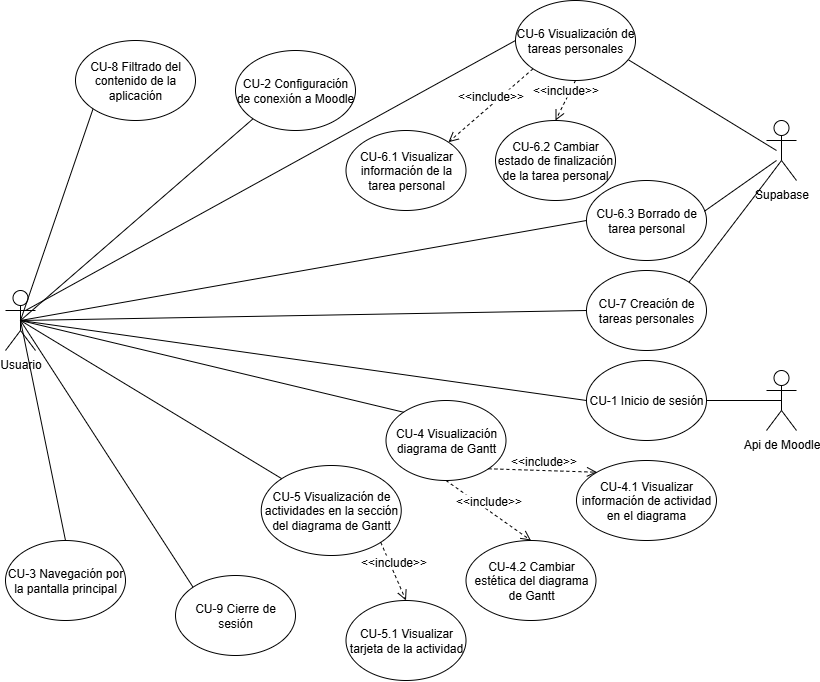
\includegraphics[width=1.0\linewidth]{img/diagrama_casos_uso.png}
    \caption{Diagrama general de los casos de uso}
    \label{fig:diagrama_casos_uso}
\end{figure}

\begin{table}[H]
	\centering
	\begin{tabularx}{\linewidth}{ p{0.21\columnwidth} p{0.71\columnwidth} }
		\toprule
		\textbf{CU-1}    & \textbf{Inicio de sesión}\\
		\toprule
		\textbf{Versión}              & 1.0    \\
            \textbf{Actor}                & Usuario, API de Moodle \\
		\textbf{Autor}                & Javier Pampliega García \\
		\textbf{Requisitos asociados} & RF-1\\
		\textbf{Descripción}          & Permitir iniciar sesión para acceder a la aplicación y para cargar los datos de Moodle. \\
		\textbf{Precondición}         & La aplicación instalada y abierta. \\
		\textbf{Acciones}             &
		\begin{enumerate}
			\def\labelenumi{\arabic{enumi}.}
			\tightlist
			\item Estar conectado a una plataforma Moodle.
			\item Introducir las credenciales de usuario.
                \item Presionar el botón de inicio de sesión.
		\end{enumerate}\\
		\textbf{Postcondición}        & Inicio de sesión con la cuenta de Moodle del usuario. \\
		\textbf{Excepciones}          & \begin{itemize}
		    \item Ausencia de plataforma Moodle configurada.
                \item Credenciales incorrectas.
                \item Ausencia de conexión a Internet.
		\end{itemize} \\
		\textbf{Importancia}          & Alta \\
		\bottomrule
	\end{tabularx}
	\caption{CU-1 Inicio de sesión}
\end{table}

\begin{table}[p]
	\centering
	\begin{tabularx}{\linewidth}{ p{0.21\columnwidth} p{0.71\columnwidth} }
		\toprule
		\textbf{CU-2}    & \textbf{Configuración de conexión a Moodle}\\
		\toprule
		\textbf{Versión}              & 1.0    \\
            \textbf{Actor}                & Usuario \\
		\textbf{Autor}                & Javier Pampliega García \\
		\textbf{Requisitos asociados} & RF-2\\
		\textbf{Descripción}          & Permitir conectar con un servidor de Moodle. \\
		\textbf{Precondición}         & La aplicación instalada y abierta, y en el panel para conectar con un servidor Moodle. \\
		\textbf{Acciones}             &
		\begin{enumerate}
			\def\labelenumi{\arabic{enumi}.}
			\tightlist
			\item Introducir la URL del servidor Moodle.
                \item Esperar la verificación de la URL.
			\item Presionar el botón Guardar.
		\end{enumerate}\\
		\textbf{Postcondición}        & Inicio de sesión con la cuenta de Moodle del usuario. \\
		\textbf{Excepciones}          & \begin{itemize}
		    \item Que no se trate de un servidor Moodle.
                \item Ausencia de conexión a Internet.
		\end{itemize} \\
		\textbf{Importancia}          & Alta \\
		\bottomrule
	\end{tabularx}
	\caption{CU-2 Configuración de conexión a Moodle}
\end{table}

\begin{table}[p]
	\centering
	\begin{tabularx}{\linewidth}{ p{0.21\columnwidth} p{0.71\columnwidth} }
		\toprule
		\textbf{CU-3}    & \textbf{Navegación por la pantalla principal}\\
		\toprule
		\textbf{Versión}              & 1.0    \\
            \textbf{Actor}                & Usuario \\
		\textbf{Autor}                & Javier Pampliega García \\
		\textbf{Requisitos asociados} & RF-4\\
		\textbf{Descripción}          & Permitir acceder a todas las funcionalidades de la aplicación desde la misma pantalla. \\
		\textbf{Precondición}         & Sesión iniciada correctamente. \\
		\textbf{Acciones}             &
		\begin{enumerate}
			\def\labelenumi{\arabic{enumi}.}
			\tightlist
			\item Pulsar el botón de la funcionalidad a la que se quiera acceder.
		\end{enumerate}\\
		\textbf{Postcondición}        & Acceso a la funcionalidad seleccionada. \\
		\textbf{Excepciones}          & \begin{itemize}
		    \item No existen excepciones.
		\end{itemize} \\
		\textbf{Importancia}          & Media \\
		\bottomrule
	\end{tabularx}
	\caption{CU-3 Navegación por la pantalla principal}
\end{table}

\begin{table}[p]
	\centering
	\begin{tabularx}{\linewidth}{ p{0.21\columnwidth} p{0.71\columnwidth} }
		\toprule
		\textbf{CU-4}    & \textbf{Visualización del diagrama de Gantt}\\
		\toprule
		\textbf{Versión}              & 1.0    \\
            \textbf{Actor}                & Usuario \\
		\textbf{Autor}                & Javier Pampliega García \\
		\textbf{Requisitos asociados} & RF-5\\
		\textbf{Descripción}          & Permitir visualizar todas las actividades (filtradas o sin filtrar) en un diagrama de Gantt. \\
		\textbf{Precondición}         & Haber accedido desde la pantalla principal. \\
		\textbf{Acciones}             &
		\begin{enumerate}
			\def\labelenumi{\arabic{enumi}.}
			\tightlist
			\item Desplazarse por el diagrama para ver todas las actividades.
		\end{enumerate}\\
		\textbf{Postcondición}        & No hay postcondiciones. \\
		\textbf{Excepciones}          & \begin{itemize}
		    \item No existen excepciones.
		\end{itemize} \\
		\textbf{Importancia}          & Alta \\
		\bottomrule
	\end{tabularx}
	\caption{CU-4 Visualización del diagrama de Gantt}
\end{table}

\begin{table}[p]
	\centering
	\begin{tabularx}{\linewidth}{ p{0.21\columnwidth} p{0.71\columnwidth} }
		\toprule
		\textbf{CU-4.1}    & \textbf{Visualizar información de actividad en el diagrama}\\
		\toprule
		\textbf{Versión}              & 1.0    \\
            \textbf{Actor}                & Usuario \\
		\textbf{Autor}                & Javier Pampliega García \\
		\textbf{Requisitos asociados} & RF-5, RF-5.1\\
		\textbf{Descripción}          & Permitir visualizar la información de una actividad directamente desde el diagrama de Gantt. \\
		\textbf{Precondición}         & Haber accedido a la pantalla del diagrama de Gantt. \\
		\textbf{Acciones}             &
		\begin{enumerate}
			\def\labelenumi{\arabic{enumi}.}
			\tightlist
			\item Localizar la actividad a visualizar.
                \item Presionar sobre el punto que representa a la actividad en el diagrama.
		\end{enumerate}\\
		\textbf{Postcondición}        & Se visualiza una ventana con la información de la actividad. \\
		\textbf{Excepciones}          & \begin{itemize}
		    \item No existen excepciones.
		\end{itemize} \\
		\textbf{Importancia}          & Media \\
		\bottomrule
	\end{tabularx}
	\caption{CU-4.1 Navegación por la pantalla principal}
\end{table}

\begin{table}[p]
	\centering
	\begin{tabularx}{\linewidth}{ p{0.21\columnwidth} p{0.71\columnwidth} }
		\toprule
		\textbf{CU-4.2}    & \textbf{Cambiar estética del diagrama de Gantt}\\
		\toprule
		\textbf{Versión}              & 1.0    \\
            \textbf{Actor}                & Usuario \\
		\textbf{Autor}                & Javier Pampliega García \\
		\textbf{Requisitos asociados} & RF-5, RF-5.2\\
		\textbf{Descripción}          & Permitir realizar cambios en la estética del diagrama para mejorar su visualización. \\
		\textbf{Precondición}         & Haber accedido a la pantalla del diagrama de Gantt. \\
		\textbf{Acciones}             &
		\begin{enumerate}
			\def\labelenumi{\arabic{enumi}.}
			\tightlist
			\item Deslizar hacia arriba el panel inferior de la pantalla.
                \item Modificar los filtros según las necesidades del usuario.
		\end{enumerate}\\
		\textbf{Postcondición}        & Cambios en la estética del diagrama de Gantt. \\
		\textbf{Excepciones}          & \begin{itemize}
		    \item No existen excepciones.
		\end{itemize} \\
		\textbf{Importancia}          & Baja \\
		\bottomrule
	\end{tabularx}
	\caption{CU-4.2 Cambiar estética del diagrama de Gantt}
\end{table}

\begin{table}[p]
	\centering
	\begin{tabularx}{\linewidth}{ p{0.21\columnwidth} p{0.71\columnwidth} }
		\toprule
		\textbf{CU-5}    & \textbf{Visualización de actividades en la sección del diagrama de Gantt}\\
		\toprule
		\textbf{Versión}              & 1.0    \\
            \textbf{Actor}                & Usuario \\
		\textbf{Autor}                & Javier Pampliega García \\
		\textbf{Requisitos asociados} & RF-6\\
		\textbf{Descripción}          & Permitir visualizar en formato tarjeta todas las actividades que aparecen en el diagrama de Gantt. \\
		\textbf{Precondición}         & Haber accedido a la pantalla del diagrama de Gantt y a la sección de actividades del diagrama. \\
		\textbf{Acciones}             &
		\begin{enumerate}
			\def\labelenumi{\arabic{enumi}.}
			\tightlist
			\item Deslizar la lista de actividades para ver todas las actividades del diagrama.
		\end{enumerate}\\
		\textbf{Postcondición}        & El usuario visualiza las actividades \\
		\textbf{Excepciones}          & \begin{itemize}
		    \item No existen excepciones.
		\end{itemize} \\
		\textbf{Importancia}          & Media \\
		\bottomrule
	\end{tabularx}
	\caption{CU-5 Visualización de actividades en la sección del diagrama de Gantt}
\end{table}

\begin{table}[p]
	\centering
	\begin{tabularx}{\linewidth}{ p{0.21\columnwidth} p{0.71\columnwidth} }
		\toprule
		\textbf{CU-5.1}    & \textbf{Visualizar tarjeta de la actividad}\\
		\toprule
		\textbf{Versión}              & 1.0    \\
            \textbf{Actor}                & Usuario \\
		\textbf{Autor}                & Javier Pampliega García \\
		\textbf{Requisitos asociados} & RF-6, RF-6.1\\
		\textbf{Descripción}          & Permitir visualizar toda la información disponible de la actividad seleccionada. \\
		\textbf{Precondición}         & Haber accedido a la pantalla del diagrama de Gantt y a la sección de actividades. \\
		\textbf{Acciones}             &
		\begin{enumerate}
			\def\labelenumi{\arabic{enumi}.}
			\tightlist
			\item Presionar sobre la tarjeta de la actividad que se quiera visualizar.
		\end{enumerate}\\
		\textbf{Postcondición}        & El usuario visualiza la información de la actividad. \\
		\textbf{Excepciones}          & \begin{itemize}
		    \item No existen excepciones.
		\end{itemize} \\
		\textbf{Importancia}          & Baja \\
		\bottomrule
	\end{tabularx}
	\caption{CU-5.1 Visualizar tarjeta de la actividad}
\end{table}

\begin{table}[p]
	\centering
	\begin{tabularx}{\linewidth}{ p{0.21\columnwidth} p{0.71\columnwidth} }
		\toprule
		\textbf{CU-6}    & \textbf{Visualización de tareas personales}\\
		\toprule
		\textbf{Versión}              & 1.0    \\
            \textbf{Actor}                & Usuario, Supabase \\
		\textbf{Autor}                & Javier Pampliega García \\
		\textbf{Requisitos asociados} & RF-7\\
		\textbf{Descripción}          & Permitir visualizar todas las tareas personales del usuario. \\
		\textbf{Precondición}         & Haber accedido desde la pantalla principal. \\
		\textbf{Acciones}             &
		\begin{enumerate}
			\def\labelenumi{\arabic{enumi}.}
			\tightlist
			\item Visualizar la sección de tareas \textit{Pendientes} y todas sus subsecciones.
                \item Visualizar la sección de tareas. \textit{Completadas} y todas sus subsecciones.
		\end{enumerate}\\
		\textbf{Postcondición}        & El usuario visualiza todas las tareas personales. \\
		\textbf{Excepciones}          & \begin{itemize}
		    \item No existen excepciones.
		\end{itemize} \\
		\textbf{Importancia}          & Alta \\
		\bottomrule
	\end{tabularx}
	\caption{CU-6 Visualización de tareas personales}
\end{table}

\begin{table}[p]
	\centering
	\begin{tabularx}{\linewidth}{ p{0.21\columnwidth} p{0.71\columnwidth} }
		\toprule
		\textbf{CU-6.1}    & \textbf{Visualizar información de la tarea personal}\\
		\toprule
		\textbf{Versión}              & 1.0    \\
            \textbf{Actor}                & Usuario \\
		\textbf{Autor}                & Javier Pampliega García \\
		\textbf{Requisitos asociados} & RF-7, RF-7.1\\
		\textbf{Descripción}          & Permitir visualizar la información asociada a la tarea que se desea revisar. \\
		\textbf{Precondición}         & Haber accedido a la pantalla del diagrama de Gantt. \\
		\textbf{Acciones}             &
		\begin{enumerate}
			\def\labelenumi{\arabic{enumi}.}
			\tightlist
			\item Presionar la tarea personal que se desea visualizar.
		\end{enumerate}\\
		\textbf{Postcondición}        & El usuario visualiza la información de la tarea personal. \\
		\textbf{Excepciones}          & \begin{itemize}
		    \item No existen excepciones.
		\end{itemize} \\
		\textbf{Importancia}          & Media \\
		\bottomrule
	\end{tabularx}
	\caption{CU-6.1 Visualizar información de la tarea personal}
\end{table}

\begin{table}[p]
	\centering
	\begin{tabularx}{\linewidth}{ p{0.21\columnwidth} p{0.71\columnwidth} }
		\toprule
		\textbf{CU-6.2}    & \textbf{Cambiar estado de finalización de la tarea personal}\\
		\toprule
		\textbf{Versión}              & 1.0    \\
            \textbf{Actor}                & Usuario \\
		\textbf{Autor}                & Javier Pampliega García \\
		\textbf{Requisitos asociados} & RF-7, RF-7.2\\
		\textbf{Descripción}          & Permitir cambiar el estado de finalización de una tarea personal. \\
		\textbf{Precondición}         & Haber accedido a la pantalla de tareas personales. \\
		\textbf{Acciones}             &
		\begin{enumerate}
			\def\labelenumi{\arabic{enumi}.}
			\tightlist
			\item Presionar la casilla circular para cambiar el estado de finalización de la tarea.
		\end{enumerate}\\
		\textbf{Postcondición}        & El usuario cambia el estado de finalización y la tarea cambia de sección, \textit{Pendiente} o \textit{Completada}. \\
		\textbf{Excepciones}          & \begin{itemize}
		    \item No existen excepciones.
		\end{itemize} \\
		\textbf{Importancia}          & Media \\
		\bottomrule
	\end{tabularx}
	\caption{CU-6.2 Cambiar estado de finalización de la tarea personal}
\end{table}

\begin{table}[p]
	\centering
	\begin{tabularx}{\linewidth}{ p{0.21\columnwidth} p{0.71\columnwidth} }
		\toprule
		\textbf{CU-6.3}    & \textbf{Borrado de tarea personal}\\
		\toprule
		\textbf{Versión}              & 1.0    \\
            \textbf{Actor}                & Usuario, Supabase \\
		\textbf{Autor}                & Javier Pampliega García \\
		\textbf{Requisitos asociados} & RF-7, RF-7.3\\
		\textbf{Descripción}          & Permitir eliminar tareas personales. \\
		\textbf{Precondición}         & Haber accedido a la pantalla de tareas personales. \\
		\textbf{Acciones}             &
		\begin{enumerate}
			\def\labelenumi{\arabic{enumi}.}
			\tightlist
			\item Deslizar hacia la izquierda la tarea personal.
                \item Presionar el icono que representa una "papelera".
		\end{enumerate}\\
		\textbf{Postcondición}        & El usuario elimina la tarea personal. \\
		\textbf{Excepciones}          & \begin{itemize}
		    \item No existen excepciones.
		\end{itemize} \\
		\textbf{Importancia}          & Media \\
		\bottomrule
	\end{tabularx}
	\caption{CU-6.3 Visualizar información de la tarea personal}
\end{table}

\begin{table}[p]
	\centering
	\begin{tabularx}{\linewidth}{ p{0.21\columnwidth} p{0.71\columnwidth} }
		\toprule
		\textbf{CU-7}    & \textbf{Creación de tareas personales}\\
		\toprule
		\textbf{Versión}              & 1.0    \\
            \textbf{Actor}                & Usuario, Supabase \\
		\textbf{Autor}                & Javier Pampliega García \\
		\textbf{Requisitos asociados} & RF-7, RF-8\\
		\textbf{Descripción}          & Permitir al usuario la creación de nuevas tareas personales. \\
		\textbf{Precondición}         & Haber accedido a la pantalla de tareas personales. \\
		\textbf{Acciones}             &
		\begin{enumerate}
			\def\labelenumi{\arabic{enumi}.}
			\tightlist
			\item Presionar el botón de la esquina inferior derecha.
                \item Rellenar los campos marcados como obligatorios (*).
                \item Presionar el botón de guardar.
		\end{enumerate}\\
		\textbf{Postcondición}        & El usuario crea una tarea personal. \\
		\textbf{Excepciones}          & \begin{itemize}
		    \item No se rellenan todos los campos obligatorios.
		\end{itemize} \\
		\textbf{Importancia}          & Alta \\
		\bottomrule
	\end{tabularx}
	\caption{CU-7 Creación de tareas personales}
\end{table}

\begin{table}[p]
	\centering
	\begin{tabularx}{\linewidth}{ p{0.21\columnwidth} p{0.71\columnwidth} }
		\toprule
		\textbf{CU-8}    & \textbf{Filtrado del contenido de la aplicación}\\
		\toprule
		\textbf{Versión}              & 1.0    \\
            \textbf{Actor}                & Usuario \\
		\textbf{Autor}                & Javier Pampliega García \\
		\textbf{Requisitos asociados} & RF-9\\
		\textbf{Descripción}          & Permitir al usuario filtrar todos los contenidos con filtros de \textit{Cursos}, \textit{Actividades}, \textit{Fechas} y \textit{Disponibilidad de fechas}. \\
		\textbf{Precondición}         & Haber iniciado sesión correctamente y estar en la pantalla principal. \\
		\textbf{Acciones}             &
		\begin{enumerate}
			\def\labelenumi{\arabic{enumi}.}
			\tightlist
			\item Presionar el botón de la parte inferior derecha de la pantalla principal.
                \item Modificar los filtros según las necesidades.
		\end{enumerate}\\
		\textbf{Postcondición}        & El usuario filtra todos los contenidos de la aplicación. \\
		\textbf{Excepciones}          & \begin{itemize}
		    \item No existen excepciones.
		\end{itemize} \\
		\textbf{Importancia}          & Alta \\
		\bottomrule
	\end{tabularx}
	\caption{CU-8 Filtrado del contenido de la aplicación}
\end{table}

\begin{table}[p]
	\centering
	\begin{tabularx}{\linewidth}{ p{0.21\columnwidth} p{0.71\columnwidth} }
		\toprule
		\textbf{CU-9}    & \textbf{Cierre de sesión}\\
		\toprule
		\textbf{Versión}              & 1.0    \\
            \textbf{Actor}                & Usuario \\
		\textbf{Autor}                & Javier Pampliega García \\
		\textbf{Requisitos asociados} & RF-3 \\
		\textbf{Descripción}          & Cerrar sesión de la aplicación. \\
		\textbf{Precondición}         & Estar situado en la pantalla principal. \\
		\textbf{Acciones}             &
		\begin{enumerate}
			\def\labelenumi{\arabic{enumi}.}
			\tightlist
			\item Presionar el botón situado en la esquina superior derecha.
		\end{enumerate}\\
		\textbf{Postcondición}        & El usuario cierra sesión correctamente en la aplicación. \\
		\textbf{Excepciones}          & \begin{itemize}
		    \item No existen excepciones.
		\end{itemize} \\
		\textbf{Importancia}          & Media \\
		\bottomrule
	\end{tabularx}
	\caption{CU-9 Cierre de sesión}
\end{table}
\apendice{Especificación de diseño}

\section{Introducción}
En este apéndice, se recoge la especificación de diseño del proyecto. El objetivo es detallar los aspectos de construcción del sistema, en el que se incluyen:
\begin{itemize}
    \item \textbf{Diseño de datos:} se definen entidades con sus atributos y relaciones entre ellas. También, se definen esquemas de persistencia.
    \item \textbf{Diseño arquitectónico:} se define la estructura interna del sistema, así como la comunicación entre los distintos módulos.
    \item \textbf{Diseño procedimental:} se definen los flujos de interacción entre el cliente y el servicio.
\end{itemize}

\section{Diseño de datos}
En esta sección, se explican los diseños de datos del sistema. A continuación, se explican las entidades que componen el sistema y las relaciones de cada una de ellas.

\subsection{Diccionario de datos}
En este proyecto solo se utiliza una tabla en la base de datos, ya que solo se desea almacenar las tareas personales de un usuario, por lo tanto, solo se requiere la utilización de una tabla. En caso de que existieran más datos a almacenar en la nube, la cantidad de tablas aumentaría.

\begin{figure}[H]
    \centering
    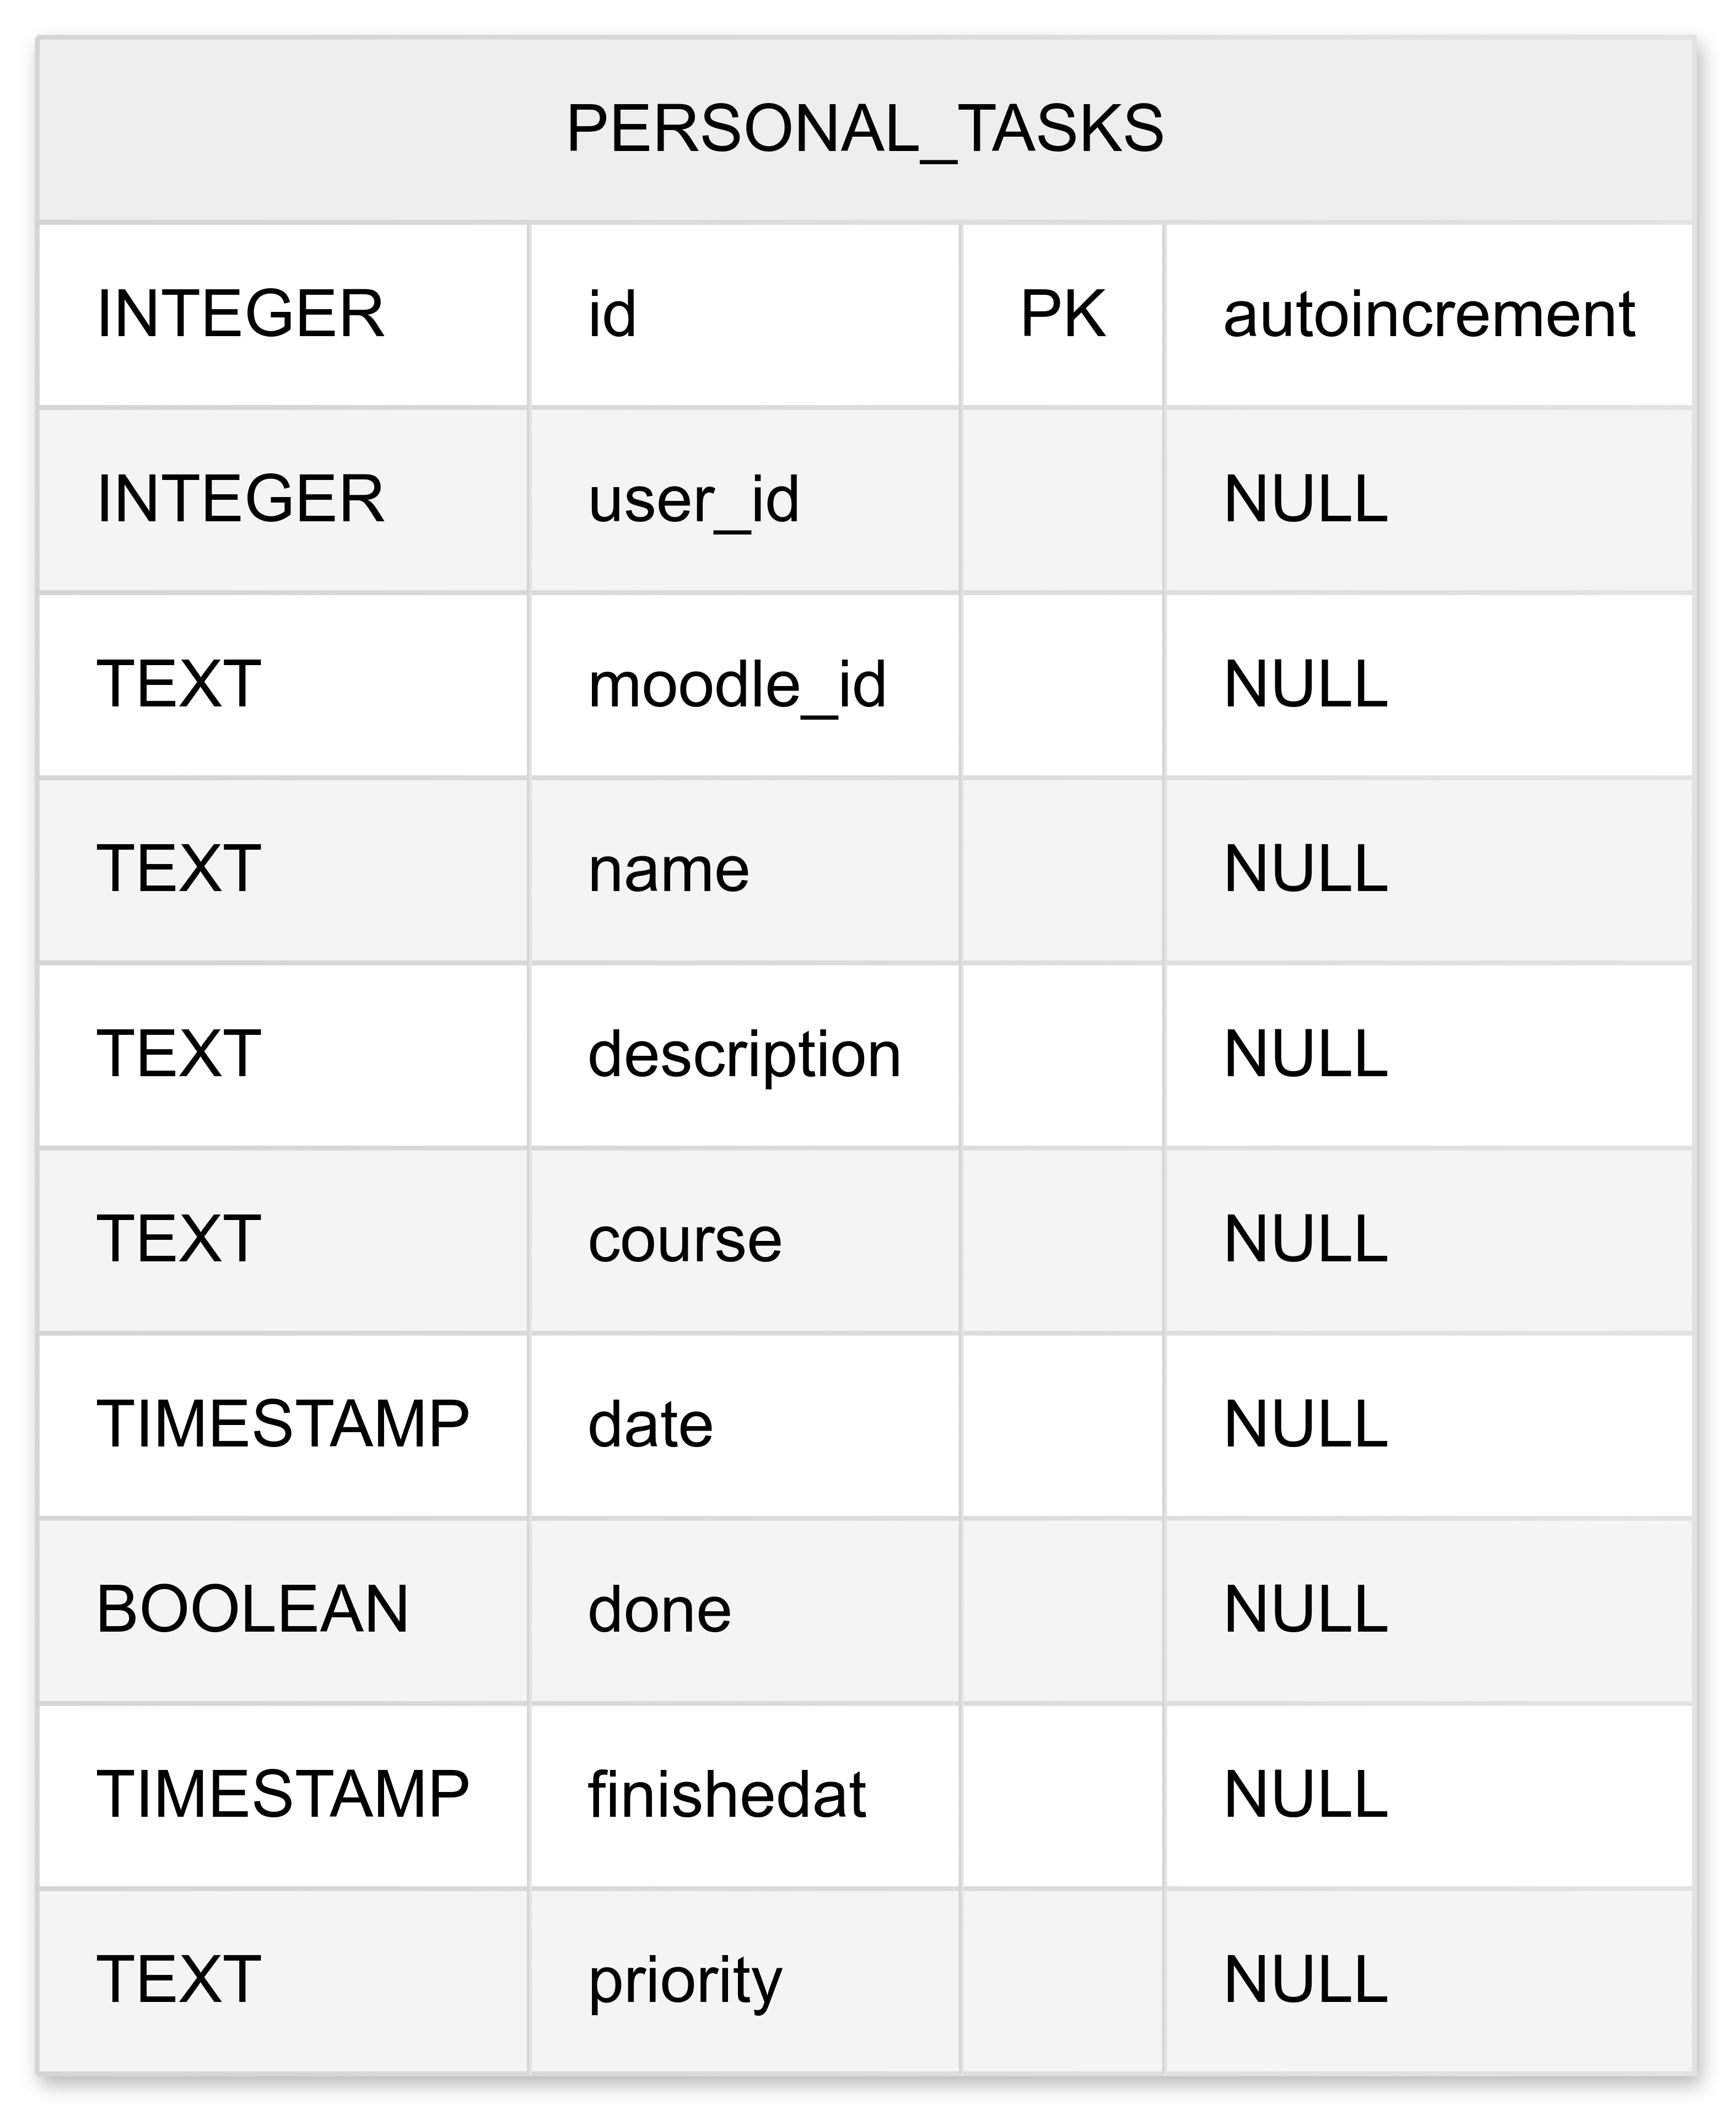
\includegraphics[width=0.6\linewidth]{img/diccionario_datos.png}
    \caption{Diccionario de datos}
    \label{fig:diccionario_datos}
\end{figure}

Se explican los atributos del diccionario de datos anterior:
\begin{itemize}
    \item \textbf{id:} representa el número de identificación de la tarea, es autoincremental Fig. \ref{fig:diccionario_datos}.
    \item \textbf{user\_id:} representa el número de identificación del usuario dentro de la plataforma en la que se encuentre Fig. \ref{fig:diccionario_datos}.
    \item \textbf{moodle\_id:} representa la URL de la plataforma a la que pertenece el usuario Fig. \ref{fig:diccionario_datos}.
    \item \textbf{name:} nombre de la tarea personal Fig. \ref{fig:diccionario_datos}.
    \item \textbf{description:} descripción de la tarea personal Fig. \ref{fig:diccionario_datos}.
    \item \textbf{course:} curso al que pertenece la tarea personal (entre los cursos en los que se encuentra matriculado el usuario propietario de la tarea personal) Fig. \ref{fig:diccionario_datos}.
    \item \textbf{date:} fecha de finalización de la tarea personal Fig. \ref{fig:diccionario_datos}.
    \item \textbf{done:} estado de finalización de la tarea Fig. \ref{fig:diccionario_datos}.
    \item \textbf{finishedat:} fecha en la que se finaliza la tarea Fig. \ref{fig:diccionario_datos}.
    \item \textbf{priority:} prioridad de la tarea Fig. \ref{fig:diccionario_datos}.
\end{itemize}

\subsection{Modelos de datos}
A continuación, se muestra un diagrama de clases para comprender la relación entre los distintos modelos de datos de la aplicación y la función de cada uno de ellos.

\begin{figure}[H]
    \centering
    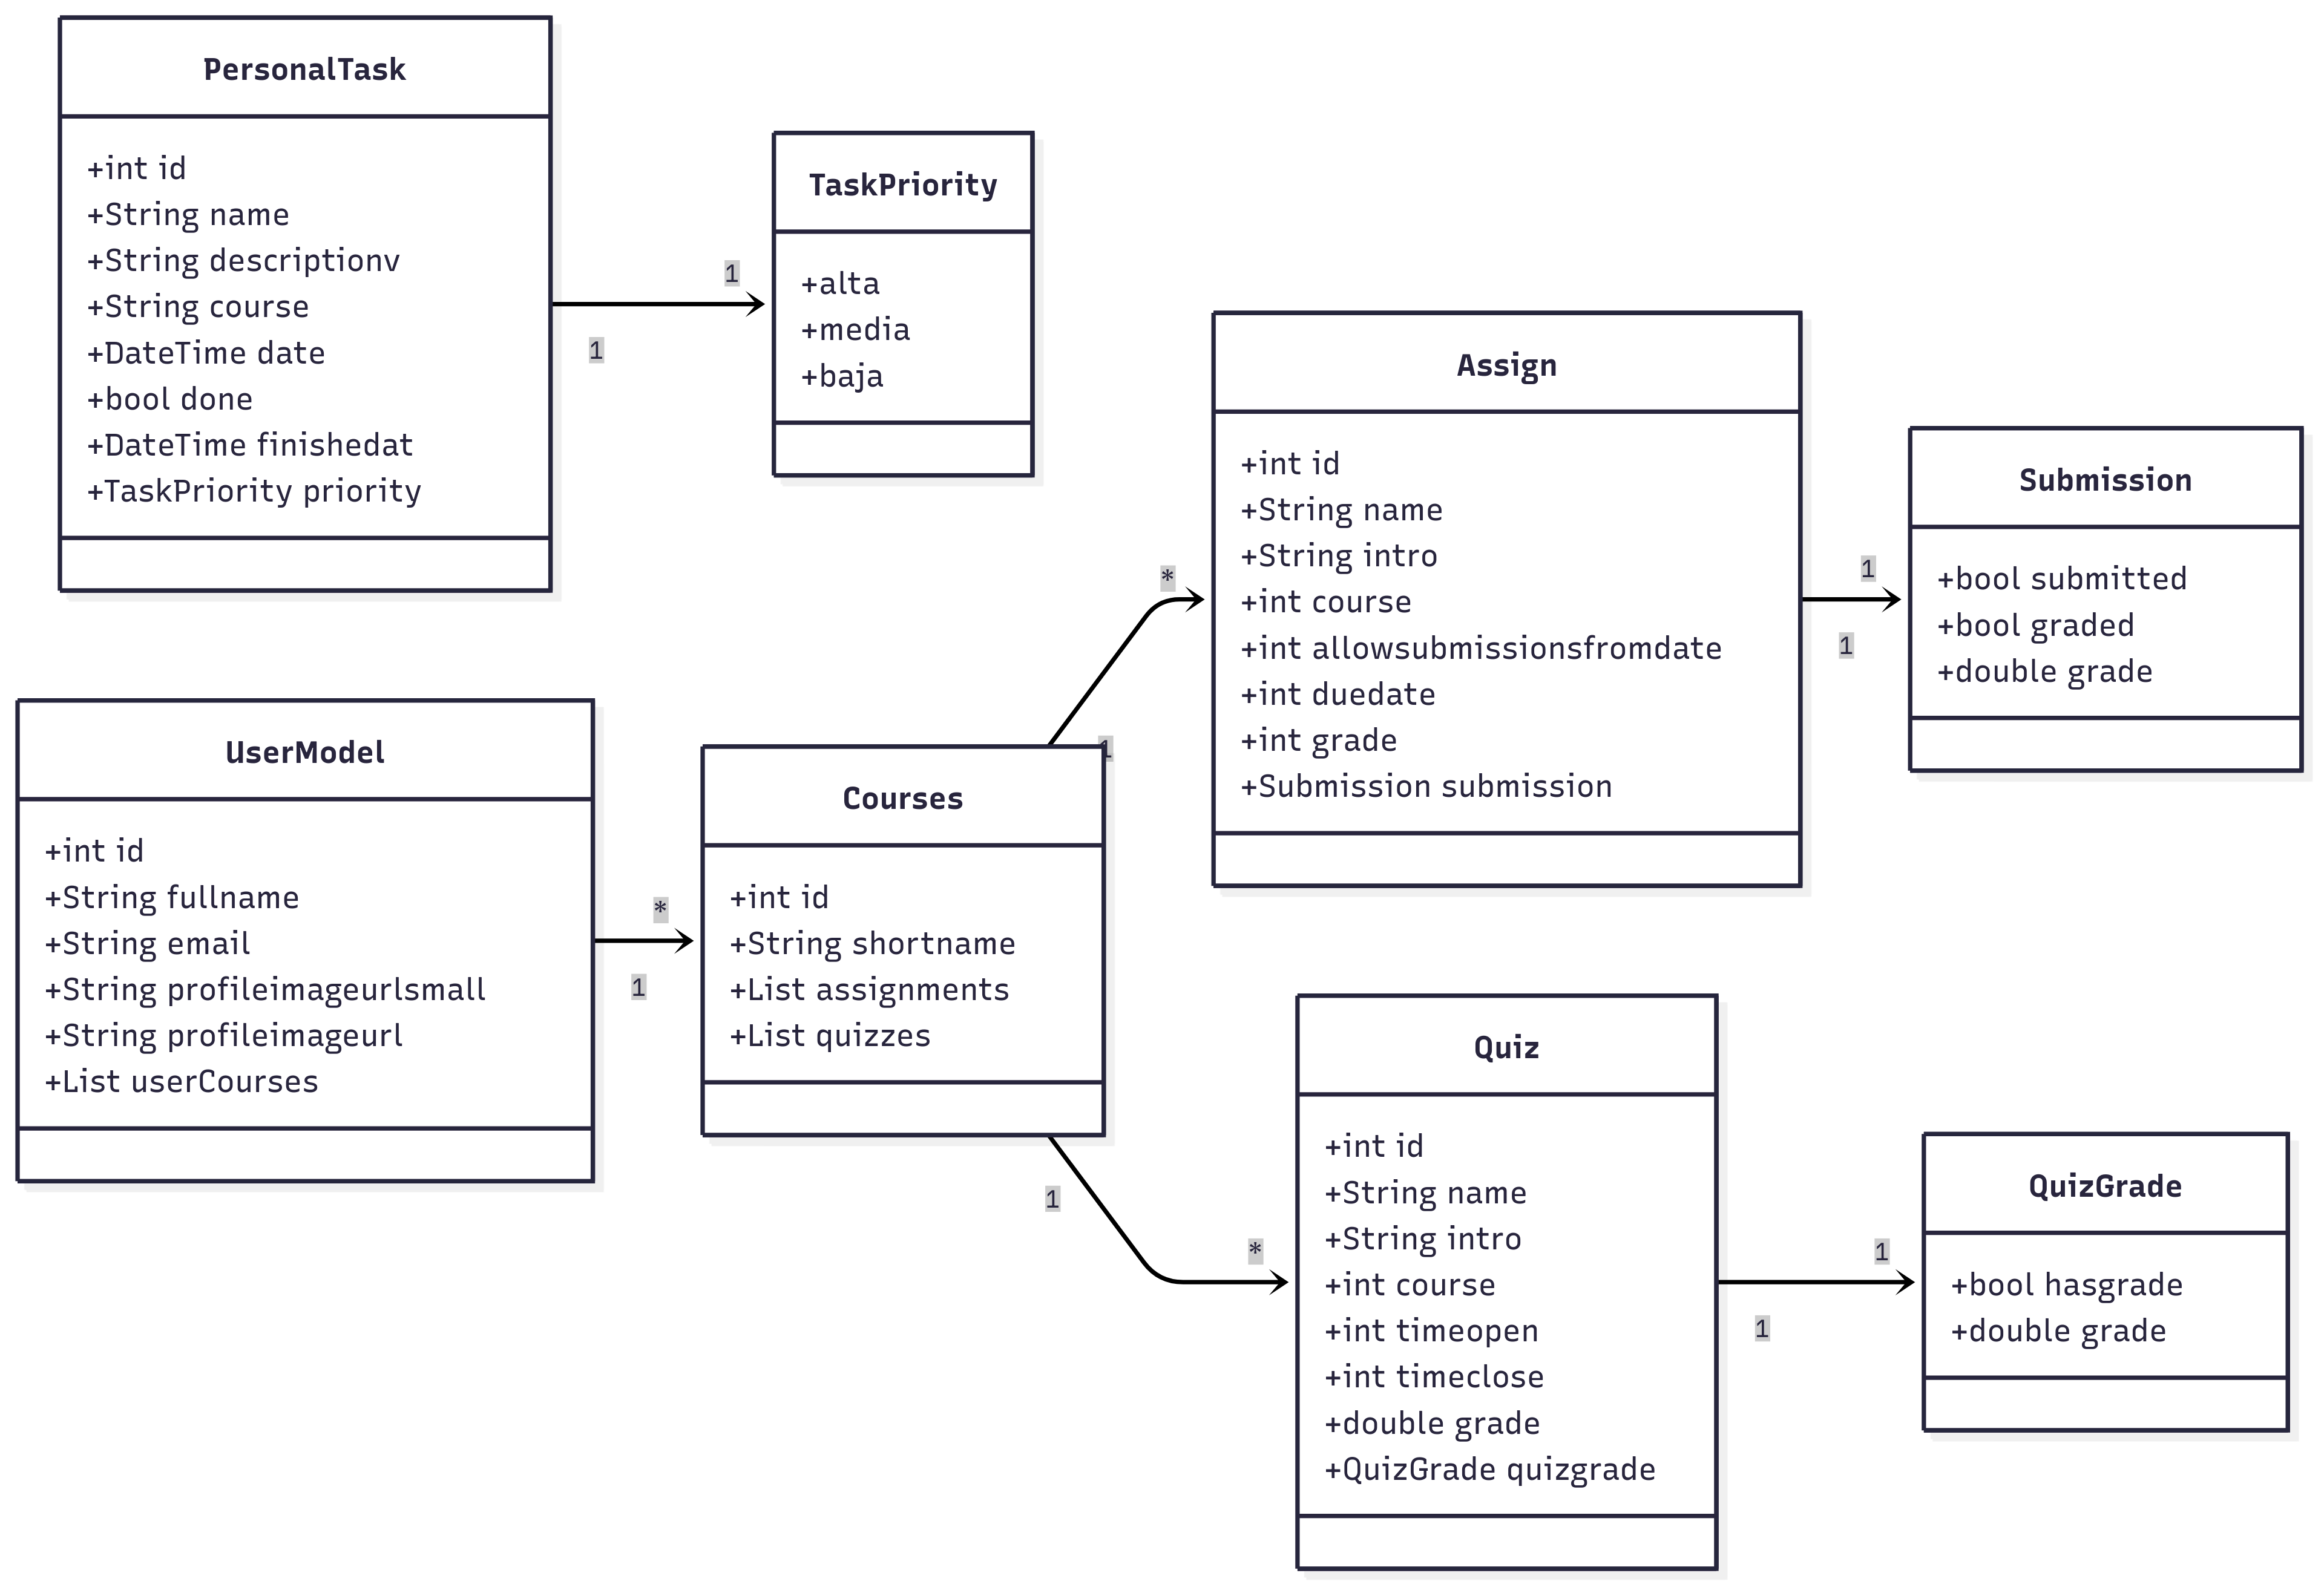
\includegraphics[width=1.0\linewidth]{img/modelo_datos.png}
    \caption{Diagrama de Modelo de datos}
    \label{fig:modelo_datos}
\end{figure}

En los modelos hay definidos más atributos, pero en el diagrama \ref{fig:modelo_datos} se representan aquellos que han sido empleados en el proyecto. A continuación se detalla cada uno de ellos:
\tablaSmallSinColores
{Modelo UserModel}
{lcc}
{modelo-usermodel}
{
    \textbf{Atributo} & \textbf{Tipo} & \textbf{Contenido} \\
}
{
    id & int & Número de identificación del usuario.\\
    fullname & String & Nombre completo del usuario.\\
    email & String & Correo electrónico del usuario.\\
    profileimageurlsmall & String & Dirección de imágen de perfil del usuario.\\
    profileimageurl & String & Dirección de imágen de perfil del usuario.\\
    userCourses & Lista & Lista de cursos del usuario.\\
}

\tablaSmallSinColores
{Modelo Courses}
{lcc}
{modelo-courses}
{
    \textbf{Atributo} & \textbf{Tipo} & \textbf{Contenido} \\
}
{
    id & int & Número de identificación del curso.\\
    shortname & String & Nombre corto del curso.\\
    assingments & Lista(Assign) & Lista de tareas del curso.\\
    quizzes & Lista(Quiz) & Lista de cuestionarios del curso.\\
}

\tablaSmallSinColores
{Modelo Assign}
{lcp{6cm}}
{modelo-assign}
{
    \textbf{Atributo} & \textbf{Tipo} & \textbf{Contenido} \\
}
{
    id & int & Número de identificación de la tarea.\\
    name & String & Nombre de la tarea.\\
    intro & String & Descripción de la tarea.\\
    course & int & Número de identificación del 
                    curso de la tarea.\\
    allowsubmissionsfromdate & int & Fecha de apertura de la tarea.\\
    duedate & int & Fecha de cierre de la tarea.\\
    grade & int & Tipo de calificación.\\
    submission & Submission & Entrega de la tarea.\\
}

\tablaSmallSinColores
{Modelo Quiz}
{lcc}
{modelo-quiz}
{
    \textbf{Atributo} & \textbf{Tipo} & \textbf{Contenido} \\
}
{
    id & int & Número de identificación del cuestionario.\\
    name & String & Nombre del cuestionario.\\
    intro & String & Descripción del cuestionario.\\
    course & int & Número de identificación del curso del cuestionario.\\
    timeopen & int & Fecha de apertura del cuestionario.\\
    timeclose & int & Fecha de cierre del cuestionario.\\
    grade & double & Tipo de calificación.\\
    quizgrade & QuizGrade & Entrega del cuestionario.\\
}

\tablaSmallSinColores
{Modelo Submission}
{lcc}
{modelo-submission}
{
    \textbf{Atributo} & \textbf{Tipo} & \textbf{Contenido} \\
}
{
    submitted & bool & Estado de entrega de la tarea.\\
    graded & bool & Estado de calificación de la entrega.\\
    grade & double & Calificación de la entrega.\\
}

\tablaSmallSinColores
{Modelo QuizGrade}
{lcc}
{modelo-quizgrade}
{
    \textbf{Atributo} & \textbf{Tipo} & \textbf{Contenido} \\
}
{
    hasgrade & bool & Estado de calificación del cuestionario.\\
    grade & double & Calificación del cuestionario.\\
}

\tablaSmallSinColores
{Modelo PersonalTask}
{lcc}
{modelo-pesonaltask}
{
    \textbf{Atributo} & \textbf{Tipo} & \textbf{Contenido} \\
}
{
    id & int & Número de identificación dela tarea personal.\\
    name & String & Nombre de la tarea personal.\\
    description & String & Descripción de la tarea personal.\\
    course & String & Nombre del curso de la tarea personal.\\
    date & DateTime & Fecha de cierre de la tarea personal.\\
    done & bool & Estado de finalización de la tarea personal.\\
    finishedat & DateTime & Fecha de finalización de la tarea personal.\\
    priority & TaskPriority & Tipo de prioridad de la tarea personal.\\
}

\tablaSmallSinColores
{Modelo TaskPriority}
{lc}
{modelo-taskpriority}
{
    \textbf{Atributo} & \textbf{Contenido} \\
}
{
    alta & Prioridad alta.\\
    baja & Prioridad media.\\
    media & Prioridad baja.\\
}

\section{Diseño arquitectónico}
El diseño arquitectónico empleado en PlanLMS se basa en una estructura modular, que persigue lograr una organización clara de las funcionalidades y responsabilidades, con el fin de garantizar la facilidad en el mantenimiento y escalabilidad del proyecto.

\begin{figure}[H]
    \centering
    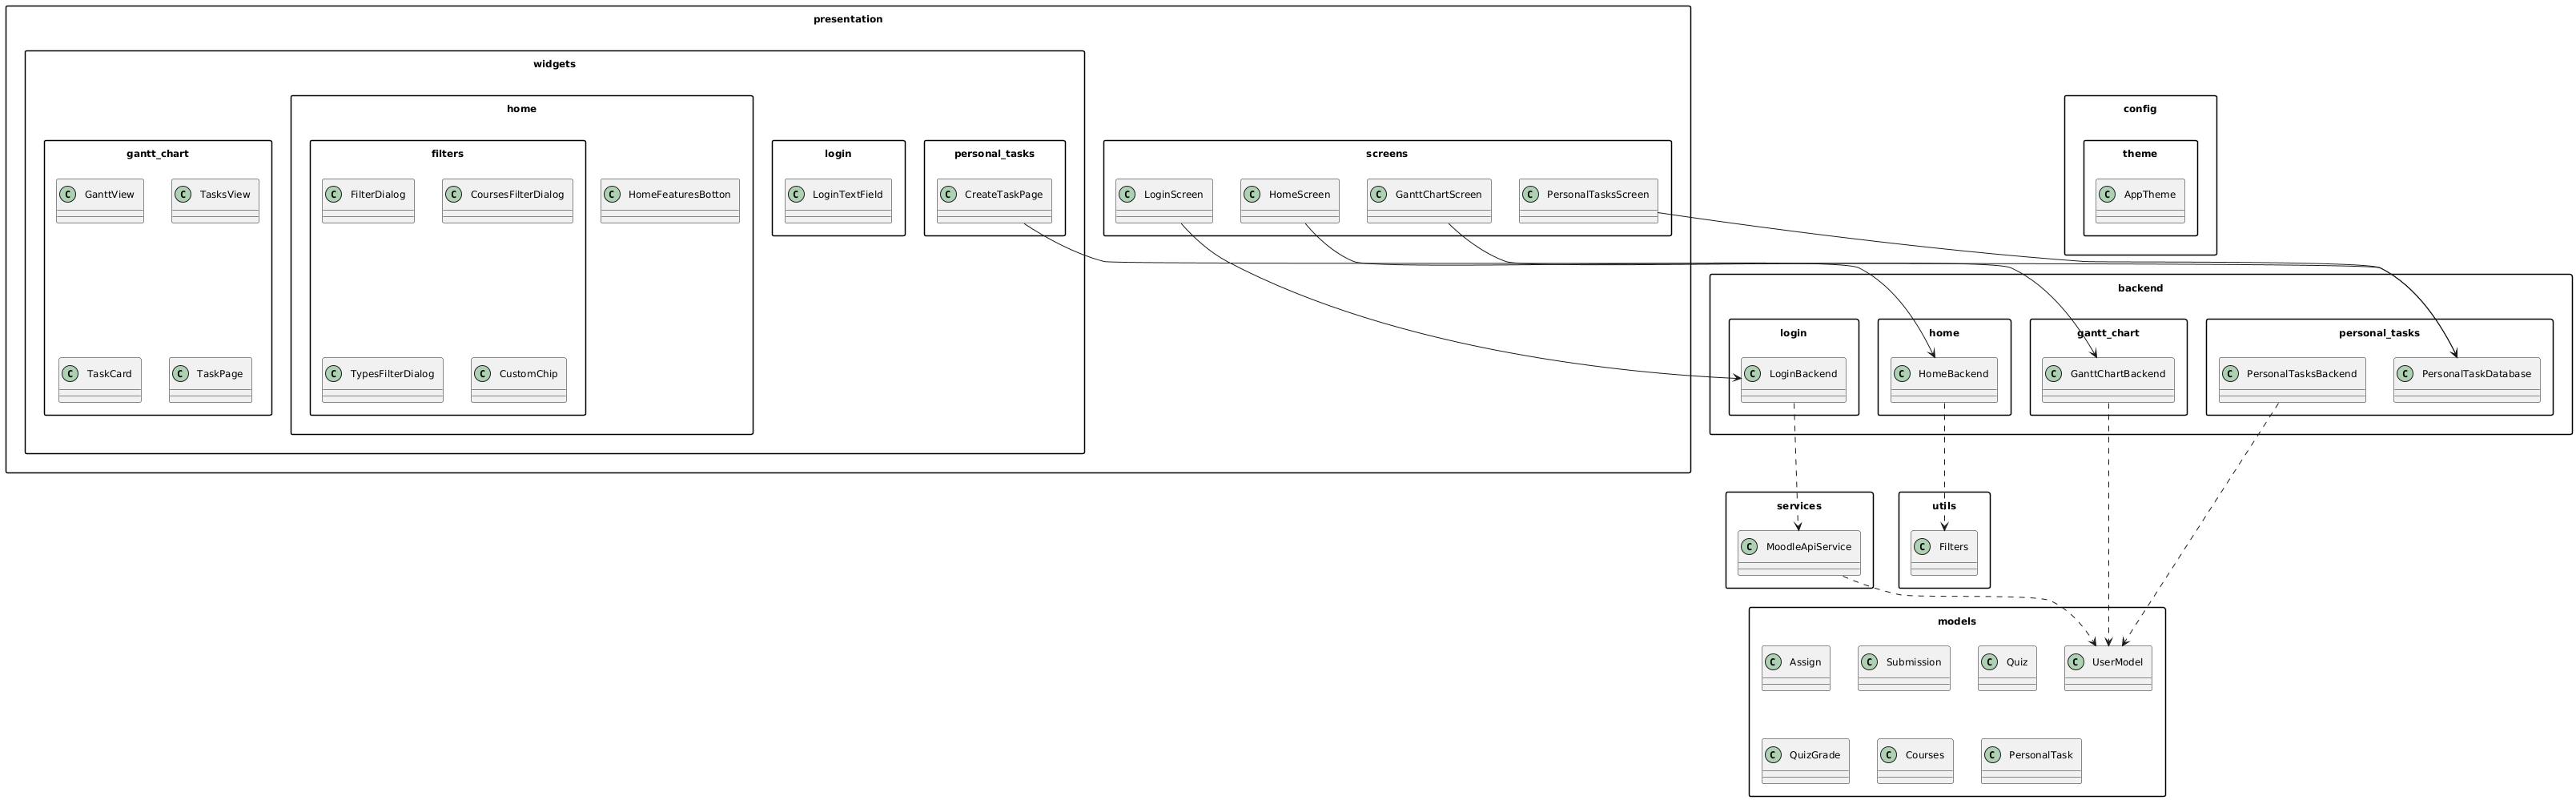
\includegraphics[width=1.3\linewidth]{img/diagrama_clases.png}
    \caption{Diseño arquitectónico del proyecto}
    \label{fig:diagrama_clases}
\end{figure}

A continuación, se detallan los objetivos de cada responsabilidad y funcionalidad:
\begin{itemize}
    \item \textbf{presentation:} contiene todos los elementos de interfaz gráfica Fig. \ref{fig:diagrama_clases}. Este paquete se divide en dos paquetes:
        \begin{itemize}
            \item \textbf{screens:} contiene las pantallas de la aplicación.
            \item \textbf{widgets:} contiene algunos widgets que componen las pantallas, con el fin de aprovechar la reutilización de estos.
        \end{itemize}
        Estos dos paquetes se dividen en otros más pequeños, cada uno asociado a una funcionalidad de la aplicación.
    \item \textbf{config:} contiene elementos de configuración de temas estéticos de algun componente Fig. \ref{fig:diagrama_clases}.
    \item \textbf{backend:} contiene la lógica de negocio, se encarga de gestionar los datos de cada capa de presentación Fig. \ref{fig:diagrama_clases}.
    \item \textbf{services:} se encarga de la comunicación con lo servicios externos Fig. \ref{fig:diagrama_clases}.
    \item \textbf{utils:} contiene los elementos que son empleados por las diferentes clases de la arquitectura Fig. \ref{fig:diagrama_clases}.
    \item \textbf{models:} contiene todas las entidades y define las estructuras de estas Fig. \ref{fig:diagrama_clases}.
\end{itemize}

\subsection{Estrategias de persistencia}
La persistencia de los datos dentro del sistema, se reparte en tres formas:
\begin{itemize}
    \item \textbf{SharedPreferences:} se encarga de almacenar los filtros de los usuarios para poder restaurarlos cada vez que se inicia la aplicación. Además, también guarda el correo electrónico de inicio de sesión.
    \item \textbf{Supabase:} se encarga de almacenar las tareas personales de todos los usuarios. Cada vez que se consulta Supabase se retorna la lista más reciente de tareas del usuario.
    \item \textbf{Caché en memoria:} se encarga de almacenar los datos de la sesión del usuario. Algunos de estos datos son los cursos, tareas, cuestionarios, entregas, calificaciones, etc.
\end{itemize}

\subsection{Seguridad}
En el directorio del proyecto existe un archivo denominado \textit{.env}, que alberga las claves para acceder a la base de datos de Supabase. Estos ficheros se excluyen de la sincronización del repositorio en la nube. Evitando que cualquier usuario no deseado pudiera acceder a los datos.

Por otra parte, el \textit{token} privado que proporciona el \textit{Web Service de Moodle} se mantiene en memoria, además, de que al cerrar sesión este se elimina de memoria.

Por último, todas las peticiones HTTP van por HTTPS, lo que quiere decir, que todas las peticiones emplean un protocolo de comunicación seguro donde los datos no van a ser leídos por terceros.

\section{Diseño procedimental}
A continuación, se muestran diagramas de secuencia que representan el funcionamiento interno de la aplicación.

\subsection{Inicio de sesión}
La Figura \ref{fig:secuencia_login} describe el comportamiento del sistema cuando el usuario inicia sesión en PlanLMS.

\begin{enumerate}
    \item El usuario introduce el correo electrónico y contraseña y presiona el botón "Iniciar sesión".
    \item \textbf{LoginScreen} le pide a su \textit{backend} que ejecute \textbf{loginSetup(email, pass, saveEmail)}, que a su vez, solicita a \textbf{MoodleAPIService} que ejecute \textbf{login(username, password)}.
    \item Una vez obtenido el \textit{token}, se almacena opcionalmente el email con \textbf{SharedPreferences}, y solicita los datos del usuario y sus cursos a \textbf{MoodleAPIService}, mediante \textbf{getUserInfo()} y \textbf{getUserCourses(userId)}.
    \item Realiza iteraciones para cada curso, obteniendo las tareas (\textbf{getCourseAssignments()}) y cuestionarios (\textbf{getCourseQuizzes()}) de cada uno, así como los estados de entrega de cada una de las actividades (\textbf{getAssignSubmissionStatus()} y \textbf{getQuizSubmissionStatus()}).
    \item Toda la información extraída, se convierte en objetos que se asignan al \textbf{UserModel} y a \textbf{Course},posteriormente se retorna a \textbf{LoginScreen} y se navega al \textbf{HomeScreen}.
\end{enumerate}

\begin{figure}[p]
    \centering
    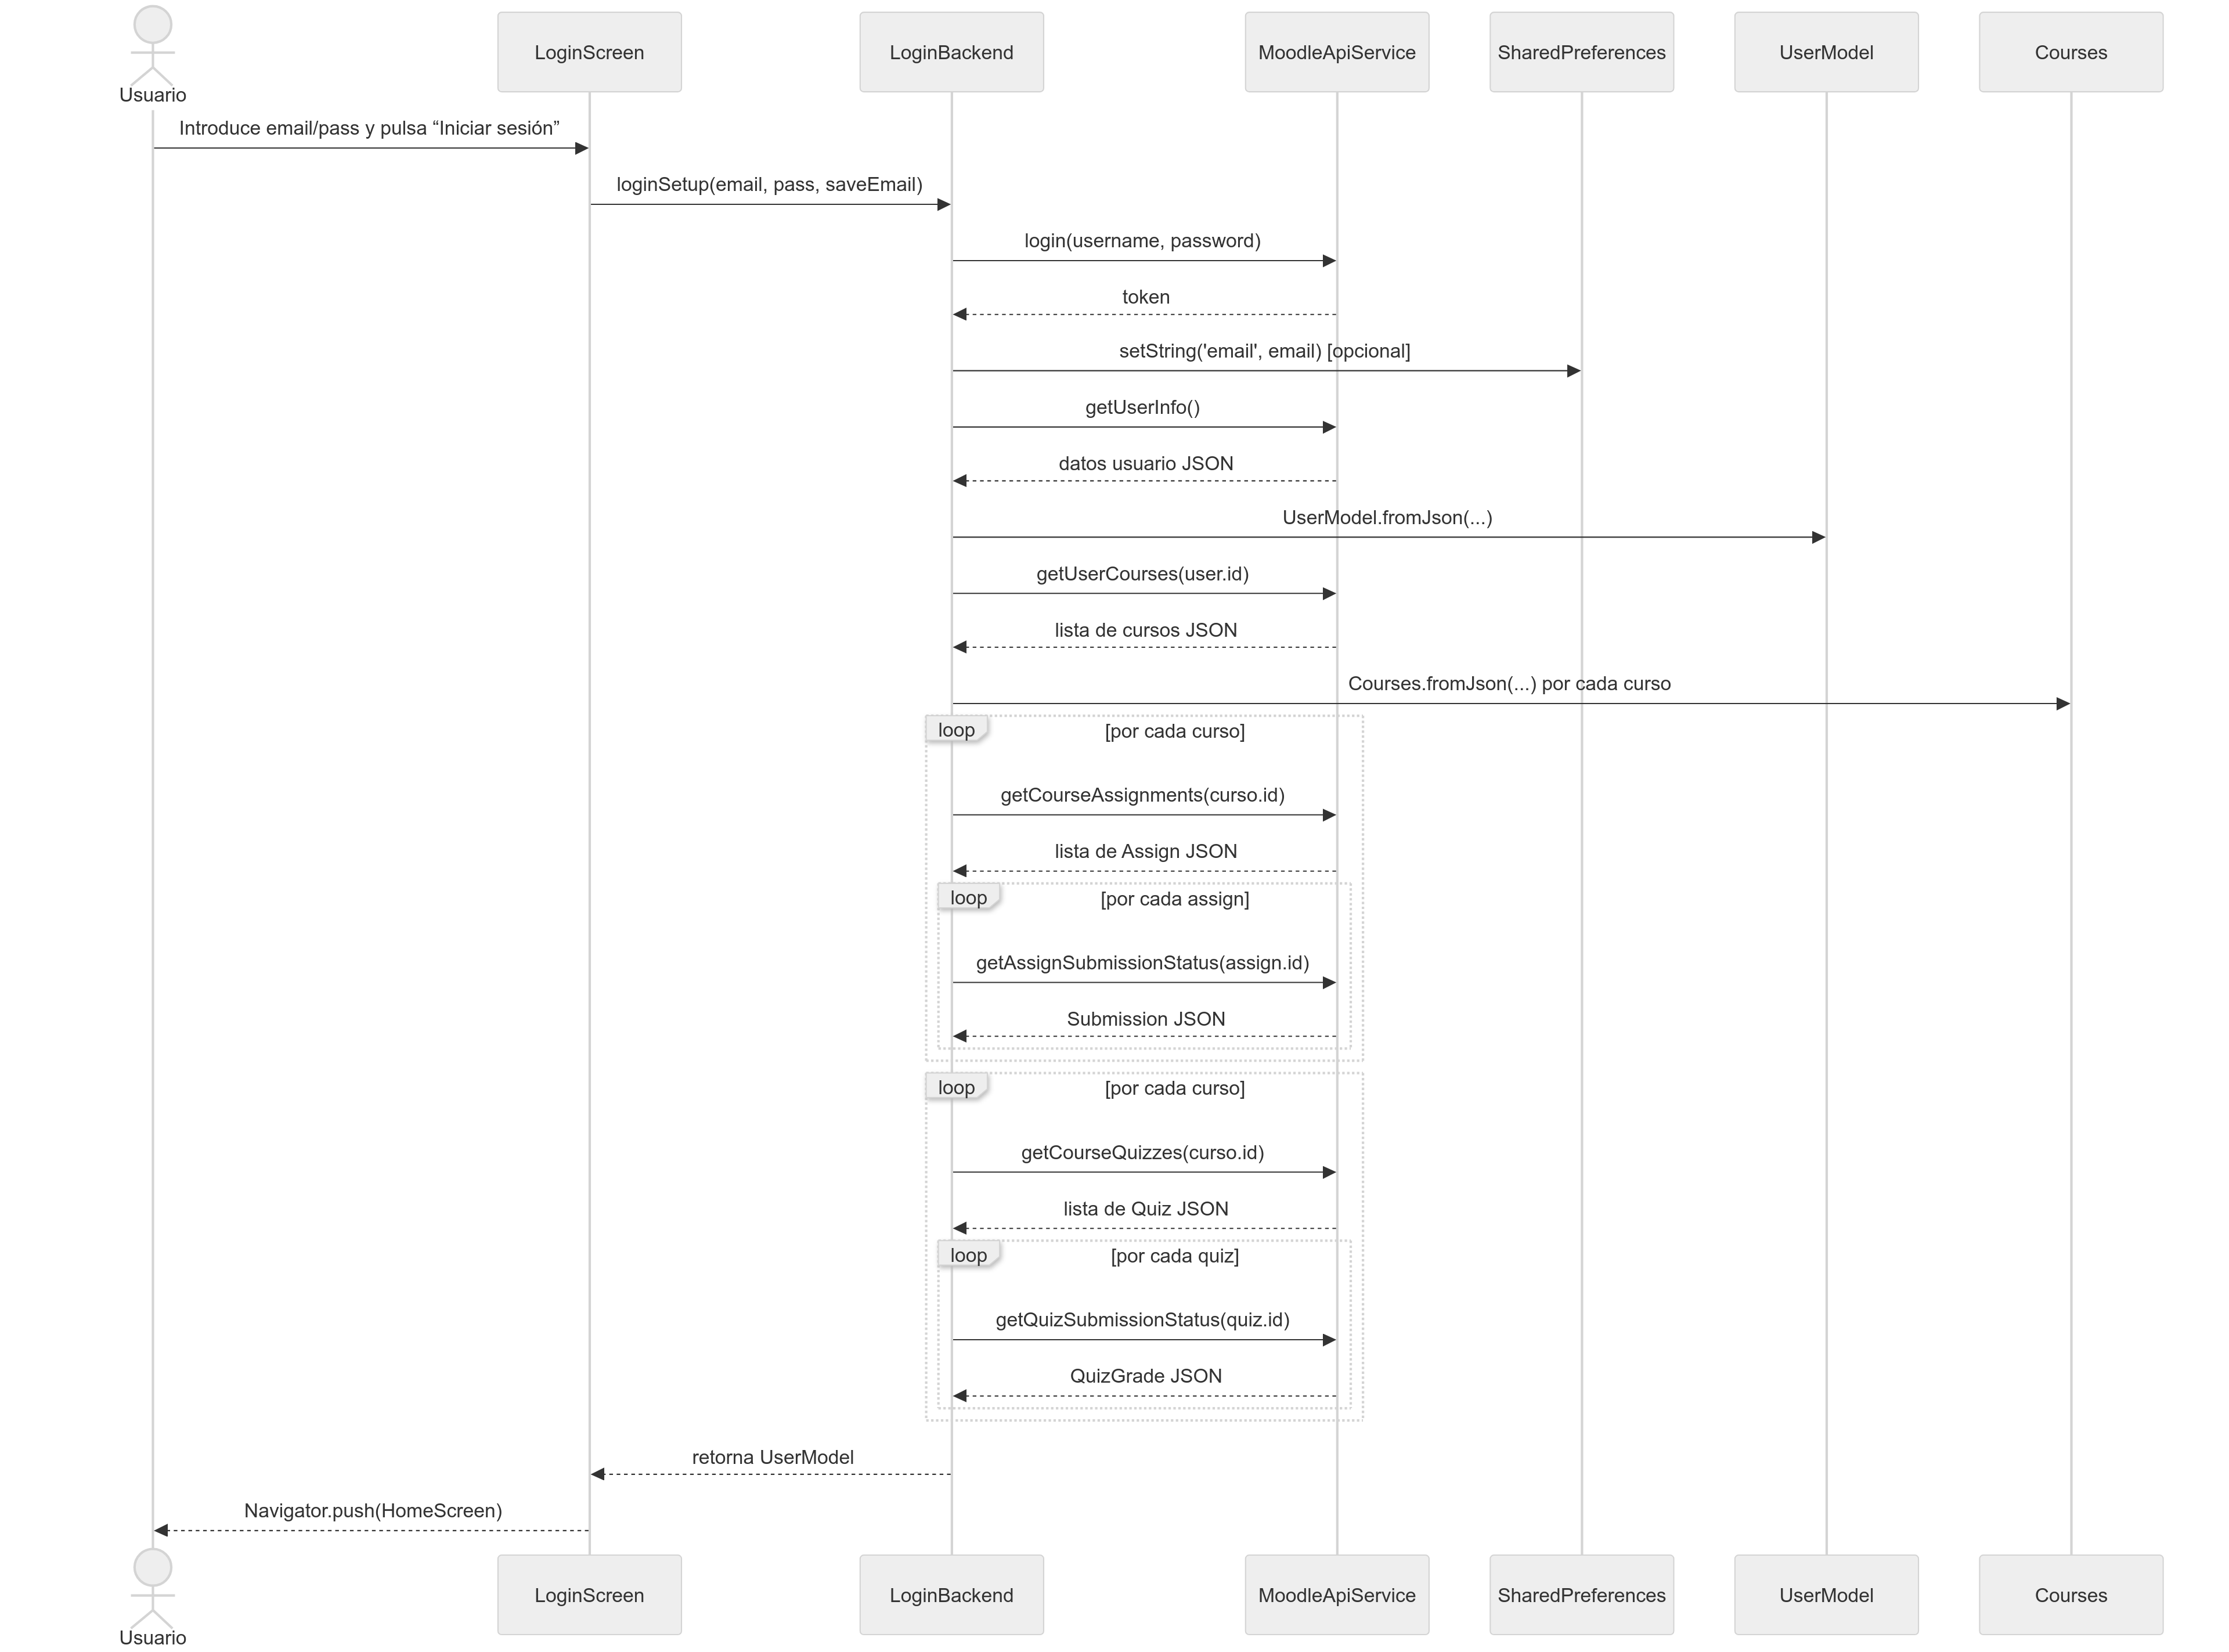
\includegraphics[width=1.2\linewidth]{img/secuencia_login.png}
    \caption{Diagrama de secuencia del inicio de sesión}
    \label{fig:secuencia_login}
\end{figure}

\subsection{Creación de tareas personales}
La Figura \ref{fig:secuencia_creacion_tareas} describe el comportamiento del sistema cuando el usuario procede con la creación de una tarea personal.

\begin{enumerate}
    \item El usuario abre el formulario y lo rellena. Al pulsar el botón \textit{Guardar} se realiza una llamada a \textbf{validateFields()} que se encarga de verificar que todos los campos del formulario han sido rellenados.
    \item Si la verificación es correcta, se ejecuta \textbf{createPersonalTask(PersonalTask)} de PersonalTaskDatabase, para realizar la inserción de la nueva tarea en la base de datos en la nube.
    \item Cuando se confirma la inserción, se realiza una llamada a \textbf{widget.refreshTasks()} que hace referencia a \textbf{loadTasks()} de \textbf{PersonalTasksScreen}, se actuliza la lista de tareas y se muestra la nueva tarea.
    \item En caso de que no se rellene el formulario con los datos necesarios, se muestra un \textbf{SnackBar} indicando \textit{Rellene los campos}.
\end{enumerate}

\begin{figure}[p]
    \centering
    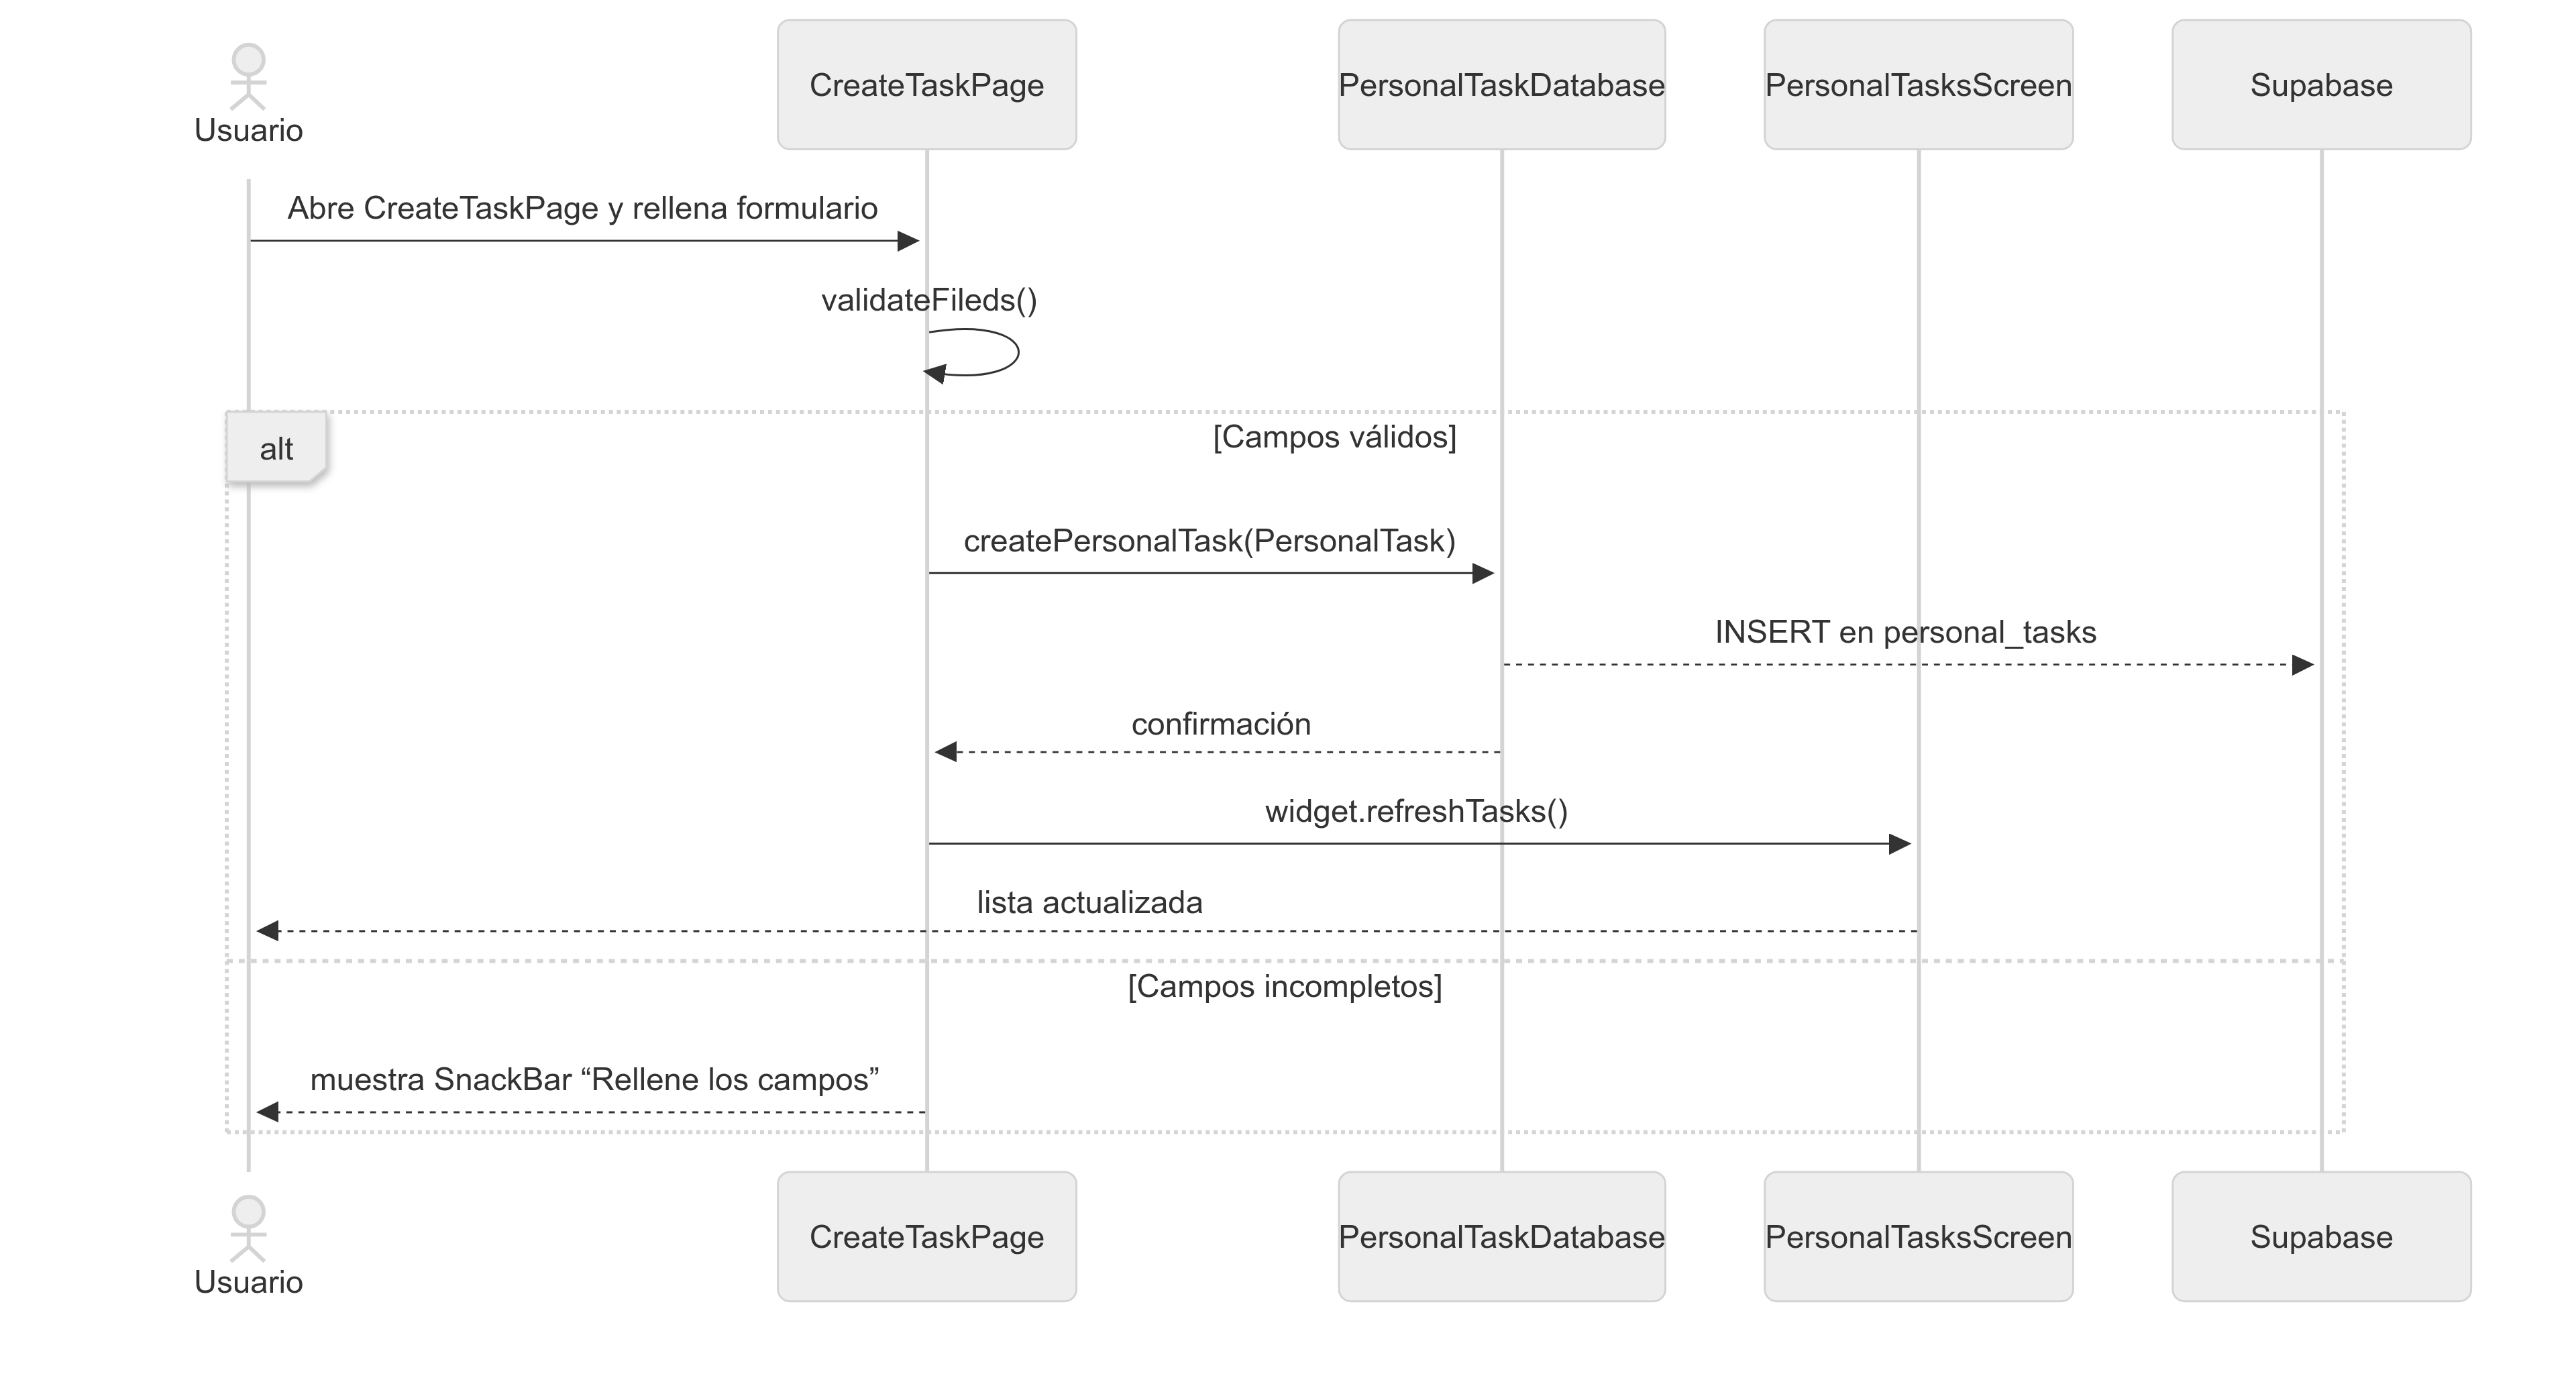
\includegraphics[width=1.0\linewidth]{img/secuencia_creacion_tareas.png}
    \caption{Diagrama de secuencia de la creación de tareas}
    \label{fig:secuencia_creacion_tareas}
\end{figure}

\subsection{Eliminación de tareas personales}
La Figura \ref{fig:secuencia_eliminar_tarea} describe el comportamiento del sistema cuando el usuario procede con la eliminación de una tarea personal.

\begin{enumerate}
    \item El usuario desliza la tarjeta de la tarea y pulsa en el icono de \textit{Eliminar}.
    \item \textbf{TaskCard} llama a la función \textbf{deleteTask(task)} de \textbf{PersonalTaskDatabase}, que solicita la base de datos eliminar la tarea personal de la tabla \textit{personal\_tasks}.
    \item Tras confirmar que se ha eliminado correctamente, se retorna de nuevo a \textbf{TaskCard}, que lanza la orden de ejecutar \textbf{refereshTasks()}, que repite el mismo proceso que la Figura \ref{fig:secuencia_creacion_tareas}.
\end{enumerate}

\begin{figure}[p]
    \centering
    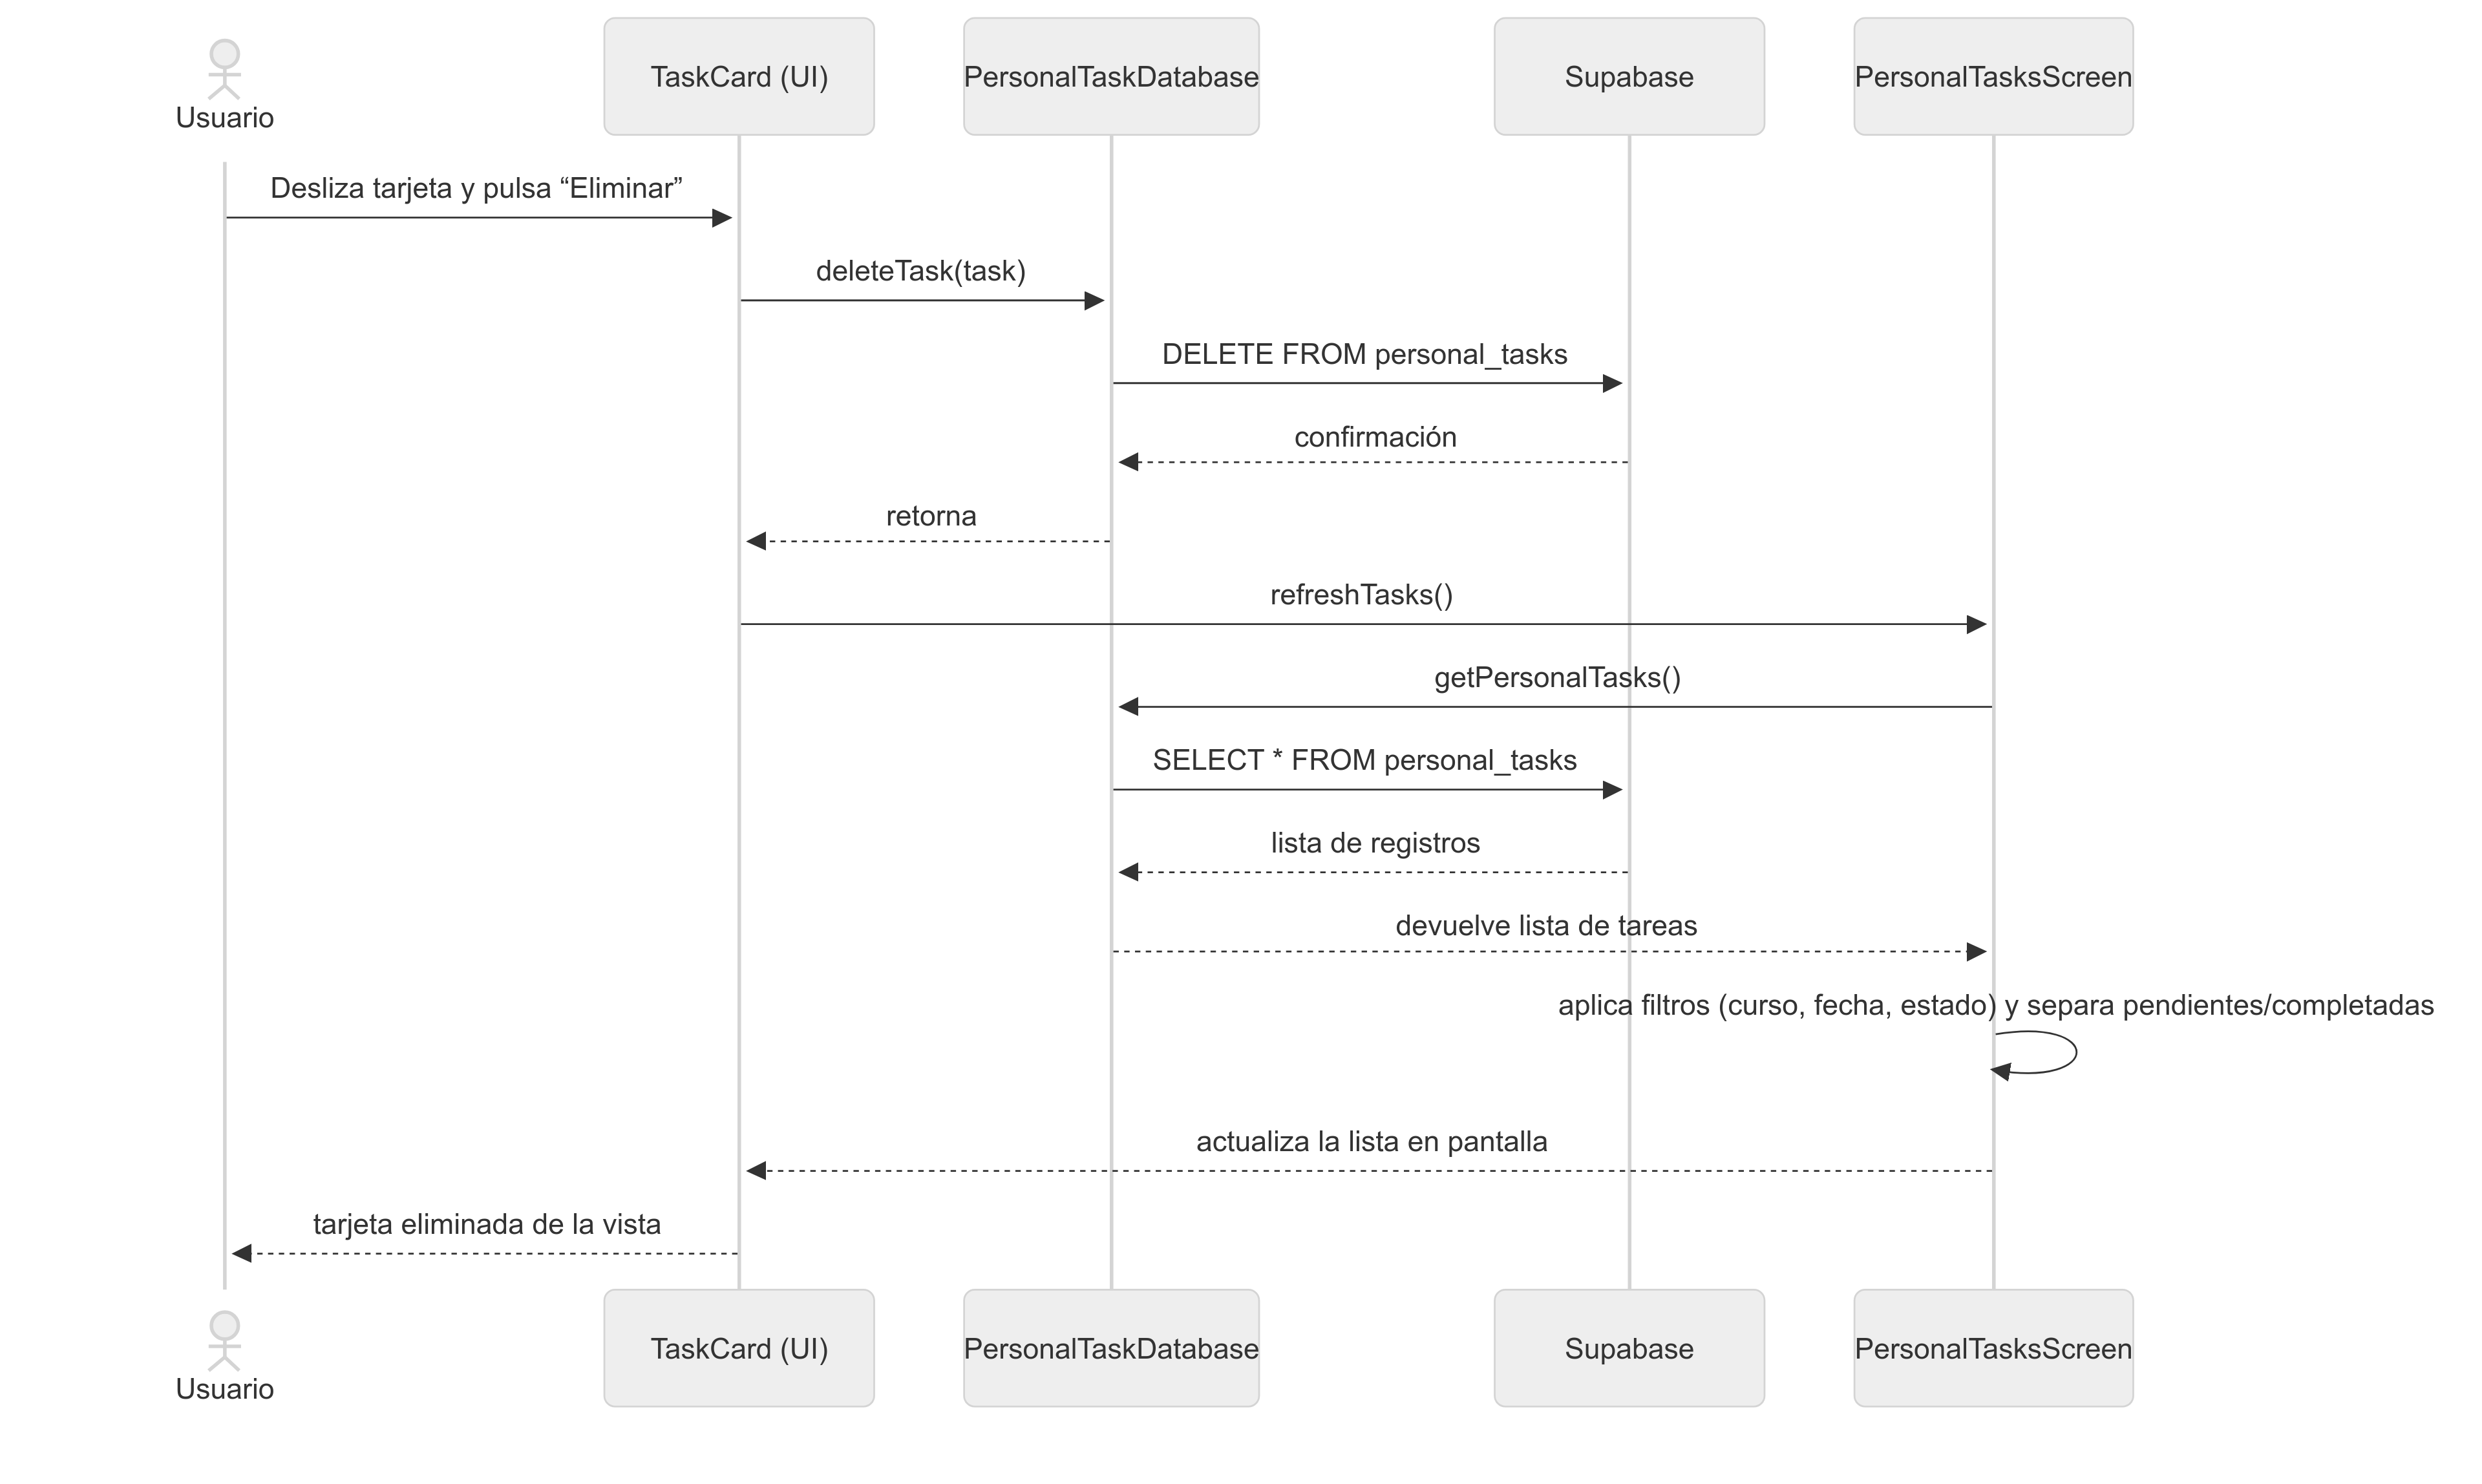
\includegraphics[width=1.0\linewidth]{img/secuencia_eliminar_tarea.png}
    \caption{Diagrama de secuencia de la eliminación de tareas}
    \label{fig:secuencia_eliminar_tarea}
\end{figure}
\apendice{Documentación técnica de programación}

\section{Introducción}
Este apéndice se centra en proporcionar una visión técnica detallada del desarrollo del proyecto. El objetivo es poder proporcionar una referencia a los futuros desarrolladores que requieran de la comprensión de la estructura del código y los procesos de compilación e instalación.

En las siguientes secciones se describen la organización de directorios del proyecto, un manual del programador con instrucciones para acceder al proyecto y sus respectivas configuraciones, y los procesos de configuración, instalación y ejecución del proyecto.

\section{Estructura de directorios}
A continuación se explican todos los directorios del \href{https://github.com/jpg1011/TFG-GestorTareasMoodle}{repositorio} del proyecto \cite{flutter_estructura}:

\begin{itemize}
    \item \textbf{app/app:} contiene todo el proyecto de Flutter. Se divide en las siguientes subcarpetas:
        \begin{itemize}
            \item \textbf{/android:} directorio generado por Flutter que contiene todos los archivos y carpetas necesarios para ejecutar la aplicación en dispositivos \textit{Android}.
            \item \textbf{/assets:} carpeta que contiene todo el contenido audiovisual de la aplicación, en este caso imágenes.
            \item \textbf{/ios:} directorio que contiene configuraciones, ejecutables, etc, que permiten ejecutar la aplicación en dispositivos \textit{iOS}.
            \item \textbf{/lib:} directorio que contiene todo el código fuente de la aplicación. Dentro de este directorio hay distintos subdirectorios, cada uno de ellos con una función:
            \begin{itemize}
                \item \textbf{/backend:} contiene el backend de cada una de las funcionalidades de la aplicación.
                \item \textbf{/config:} contiene ficheros de configuración de la aplicación.
                \item \textbf{/models:} contiene ficheros que representan cada uno de los modelos de la aplicación.
                \item \textbf{/presentation:} contiene todas las capas de presentación de \textit{UI}, dentro de esta carpeta se distinguen:
                    \begin{itemize}
                        \item \textbf{/screens:} representación de las pantallas de la aplicación, donde cada funcionalidad tiene su propio directorio.
                        \item \textbf{/widgets:} se dividen en directorios por cada funcionalidad, en cada directorio hay \textit{widgets} para mejorar la reutilización.
                    \end{itemize}
                \item \textbf{/services:} contiene el fichero que se encarga de comunicarse con la API de Moodle.
                \item \textbf{/utils:} contiene un fichero con elementos comunes en toda la aplicación.
            \end{itemize}
            \item \textbf{/linux:} directorio que contiene todo lo relacionado a configuraciones de \textit{Linux} para por ejecutar la aplicación en este entorno.
            \item \textbf{/macos:} directorio que contiene todo lo relacionado al sistema operativo de \textit{MacOS} para por ejecutar la aplicación en este entorno.
            \item \textbf{/windows:} este directorio contiene todos los archivos que permiten ejecutar la aplicación en \textit{Windows}.
        \end{itemize}
    \item \textbf{docs:} contiene todos los documentos \LaTeX 
\end{itemize}

\section{Manual del programador}
En esta sección se detallan todos los pasos a seguir para instalar y ejecutar localmente el proyecto correctamente.

\subsubsection{Configuración del entorno}
A continuación se explican todos los pasos a seguir para instalar el proyecto desde el repositorio de \textit{GitHub}.

Antes de instalar el proyecto en el equipo, es necesario tener instalado el editor de código Visual Studio Code, así como Git, posteriormente se indicarán las extensiones recomendables para el uso de \textit{Dart} y \textit{Flutter}.

Por otra parte, es necesario tener instalado en el equipo tanto \textit{Dart} como \textit{Flutter}. En este caso, no es necesario hacer una instalación directa de \textit{Dart}, ya que viene incluido en la instalación de \textit{Flutter}.

El primer paso es acceder a la \href{https://docs.flutter.dev/install/manual}{página de instalación de Flutter} y descargar el instalador del sistema que se esté utilizando. Se recomienda crear una carpeta para almacenar el \textit{SDK}. Se debe de extraer el \textit{SDK} del \textit{zip} en la carpeta creada. Por último, se crea una variable de entorno en el \textit{PATH} haciendo referencia a la ruta de la carpeta: \verb|<ruta_carpeta>\flutter\bin| \cite{flutter_instalacion}.

Para comprobar si la instalación se ha realizado con éxito, introduce el siguiente comando:
\begin{verbatim}
    flutter doctor
\end{verbatim}
Este comando realiza un diagnostico de la instalación y configuración del entorno. En caso de que falte algún elemento, se mostrará por pantalla y se deberá de proceder a su instalación.

Por otra parte, en Visual Studio Code se deben de instalar las extensiones \textit{Dart} y \textit{Flutter}, que permiten hacer uso de \textit{Dart} y \textit{Flutter}, ademas de facilitar el desarrollo al incluir atajos.

\subsubsection{Instalación del proyecto}

A continuación se procederá a la instalación del proyecto. Para ello, se debe de realizar una clonación del repositorio del proyecto. Para ello, se utiliza una terminal de comandos y se introducirá el siguiente comando:
\begin{verbatim}
git clone https://github.com/jpg1011/TFG-GestorTareasMoodle.git
\end{verbatim}

Posteriormente a la instalación del proyecto, se accederá a la carpeta de proyecto mediante el siguiente comando:
\begin{verbatim}
    cd TFG-GestorTareasMoodle/app/app
\end{verbatim}

Por último, ejecutar el siguiente comando, que abrirá el editor de código:
\begin{verbatim}
    code .
\end{verbatim}

\section{Compilación y ejecución del proyecto}
En esta sección se describen los pasos a seguir para compilar y ejecutar el proyecto. Se incluye una configuración del emulador para simular la aplicación en entornos Android.

\subsubsection{Configuración de simulador}
Para poder disponer de un emulador Android, primero es necesario instalar Android Studio, desde el cual se creará el emulador.

Una vez instalado Android Studio, se accede a la sección de emuladores desde el siguiente botón:
\begin{figure}[H]
    \centering
    
\includegraphics[width=0.7\linewidth]{img/boton_emulador.png}
    \caption{Botón de acceso a la configuración de emuladores}
    \label{fig:boton_emulador}
\end{figure}

Posteriormente, aparecerá la sección de emuladores y se debe de presionar el siguiente botón para añadir un nuevo emulador.
\begin{figure}[H]
    \centering
    \includegraphics[width=0.7\linewidth]{img/añadir_emulador.png}
    \caption{Botón para añadir nuevos emuladores}
    \label{fig:añadir_emulador}
\end{figure}

Una vez presionado el botón (imagen \ref{fig:añadir_emulador}), se selecciona la opción \textit{Create Virtual Device}.

A continuación, aparecerá una ventana con todas las imágenes de sistema disponibles para instalar en el emulador. Se seleccionará la siguiente imagen:
\begin{figure}[H]
    \centering
    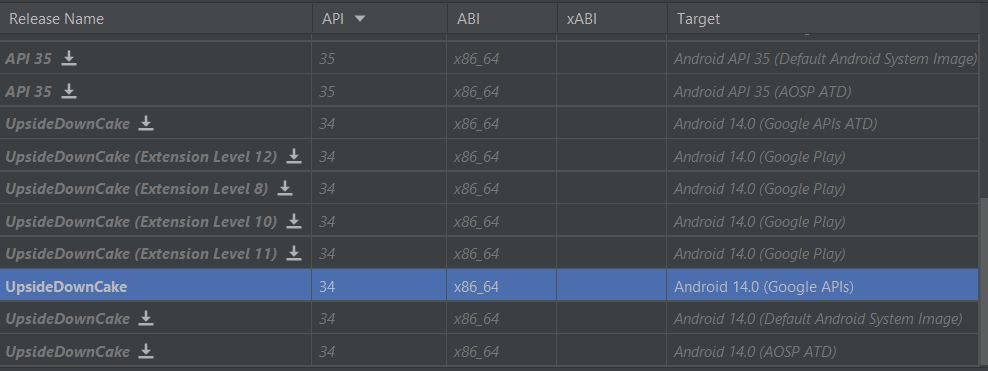
\includegraphics[width=0.7\linewidth]{img/system_image.png}
    \caption{Ventana con imágenes del sistema}
    \label{fig:system_images}
\end{figure}

Por último, aparecerá una pantalla de configuraciones generales del emulador. En este caso, se dejará todo de la misma forma.
\begin{figure}[H]
    \centering
    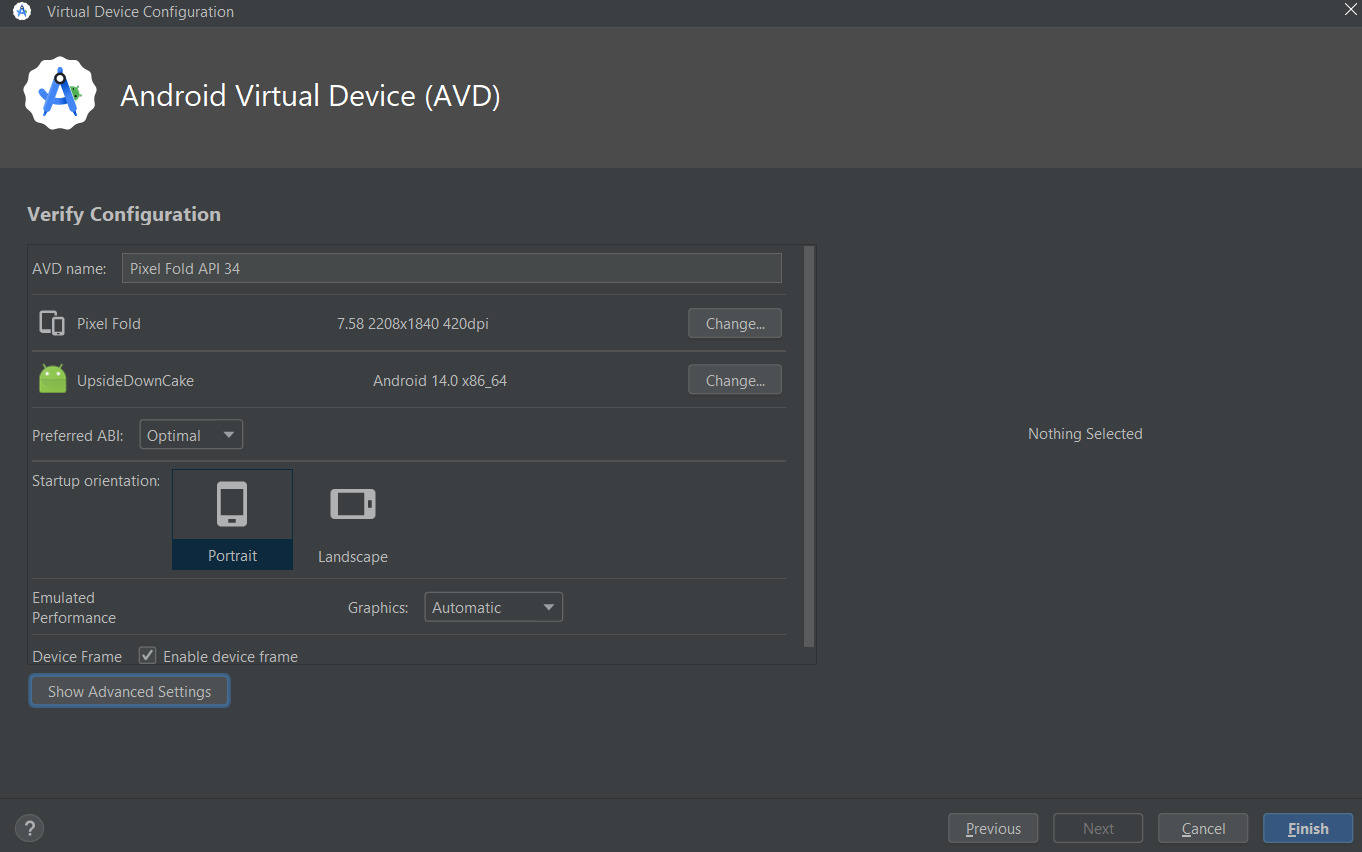
\includegraphics[width=0.9\linewidth]{img/pantalla_final_emulador.png}
    \caption{Ventana de configuración general del emulador}
    \label{fig:pantalla_final_emulador}
\end{figure}

\subsubsection{Instalación de dependencias}
Para poder ejecutar la aplicación es necesario tener instaladas las dependencias requeridas por la aplicación.

Para ello, será necesario ejecutar por terminal el siguiente comando:
\begin{verbatim}
    flutter pub get
\end{verbatim}

Tras la instalación de las dependencias se puede proceder con la ejecución de la aplicación.

\subsubsection{Ejecución de la aplicación}
A continuación se detallan los pasos necesarios para poder ejecutar la aplicación en el emulador instalador previamente.
El primer paso es pulsar la combinación de teclas \verb|Ctrl + Shift + P|. Se mostrará una ventana con un campo de texto en el que hay que introducir: \textit{Flutter: Launch Emulator}.
\begin{figure}[H]
    \centering
    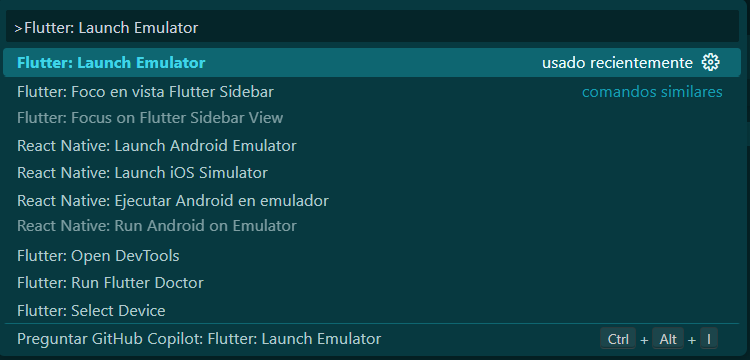
\includegraphics[width=0.9\linewidth]{img/launch_emulator.png}
    \caption{Ventana de opciones de usuario}
    \label{fig:launch_emulator}
\end{figure}

Seleccionando la opción anterior, se desplegará una lista con los emuladores disponibles, donde debería de aparecer el emulador creado anteriormente.
\begin{figure}[H]
    \centering
    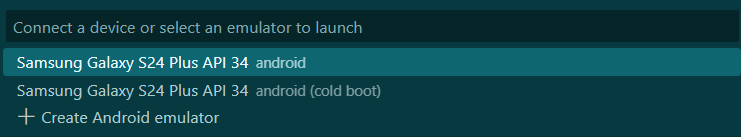
\includegraphics[width=0.9\linewidth]{img/lista_emuladores.png}
    \caption{Lista con todos los emuladores disponibles}
    \label{fig:lista_emuladores}
\end{figure}

Se iniciará el emulador, y el último paso es lanzar la aplicación con el siguiente comando.
\begin{verbatim}
    flutter run
\end{verbatim}
\apendice{Documentación de usuario}

\section{Introducción}
Este apéndice tiene como objetivo brindar a los usuarios los pasos necesarios para instalar y utilizar \textit{PlanLMS}. Se incluye a continuación información detallada sobre los requisitos mínimos para ejecutar la aplicación, pasos que el usuario debe seguir para instalar la aplicación en su dispositivo y una guía de uso.

\section{Requisitos de usuarios}
En esta sección se describen los requisitos mínimos que debe de cumplir el dispositivo del usuario para poder ejecutar correctamente \textit{PlanLMS}.

\subsection{Requisitos del Sistema} 
\begin{itemize}
    \item \textbf{Versión mínima Android:} 5.0 (API 21, \textit{Lollipop})
    \item \textbf{Versión objetivo Android:} 14.0 (API 34, \textit{Upside Down Cake})
\end{itemize}

\subsection{Requisitos Hardware}
La aplicación requiere de un dispositivo con acceso a Internet para la obtención de los datos del usuario de Moodle, así como la gestión de tareas personales, es decir, la comunicación con la base de datos.

\section{Instalación}
Actualmente la aplicación dispone de los archivos de instalación para dispositivos Android, estos se encuentran en la sección \textit{Releases} en el repositorio de GitHub.

\begin{enumerate}
    \item Acceder al siguiente repositorio de GitHub: \url{https://github.com/jpg1011/TFG-GestorTareasMoodle}.
    \item Acceder a la sección de \textit{Releases}, que se encuentra en la parte derecha.
    \item Localizar la versión más reciente y acceder a \textit{Assets}.
    \item Descargar el archivo con extensión \texttt{.apk}.
    \item Una vez descargado el archivo en el dispositivo, abrir el archivo para proceder con la instalación.

    Es necesario tener activada la opción \textit{Permitir aplicaciones de fuentes desconocidas}.
    \item Seguir la instrucciones del dispositivo para finalizar la instalación.
\end{enumerate}

\section{Manual del usuario}
A continuación, se describen todas las acciones que puede realizar un usuario de PlanLMS. Se detallarán todas las funcionalidades, así como todos los pasos a seguir para poder usar de forma eficiente cada una de las funcionalidades.

\subsection{Inicio de sesión}
\begin{figure}[H]
    \centering
    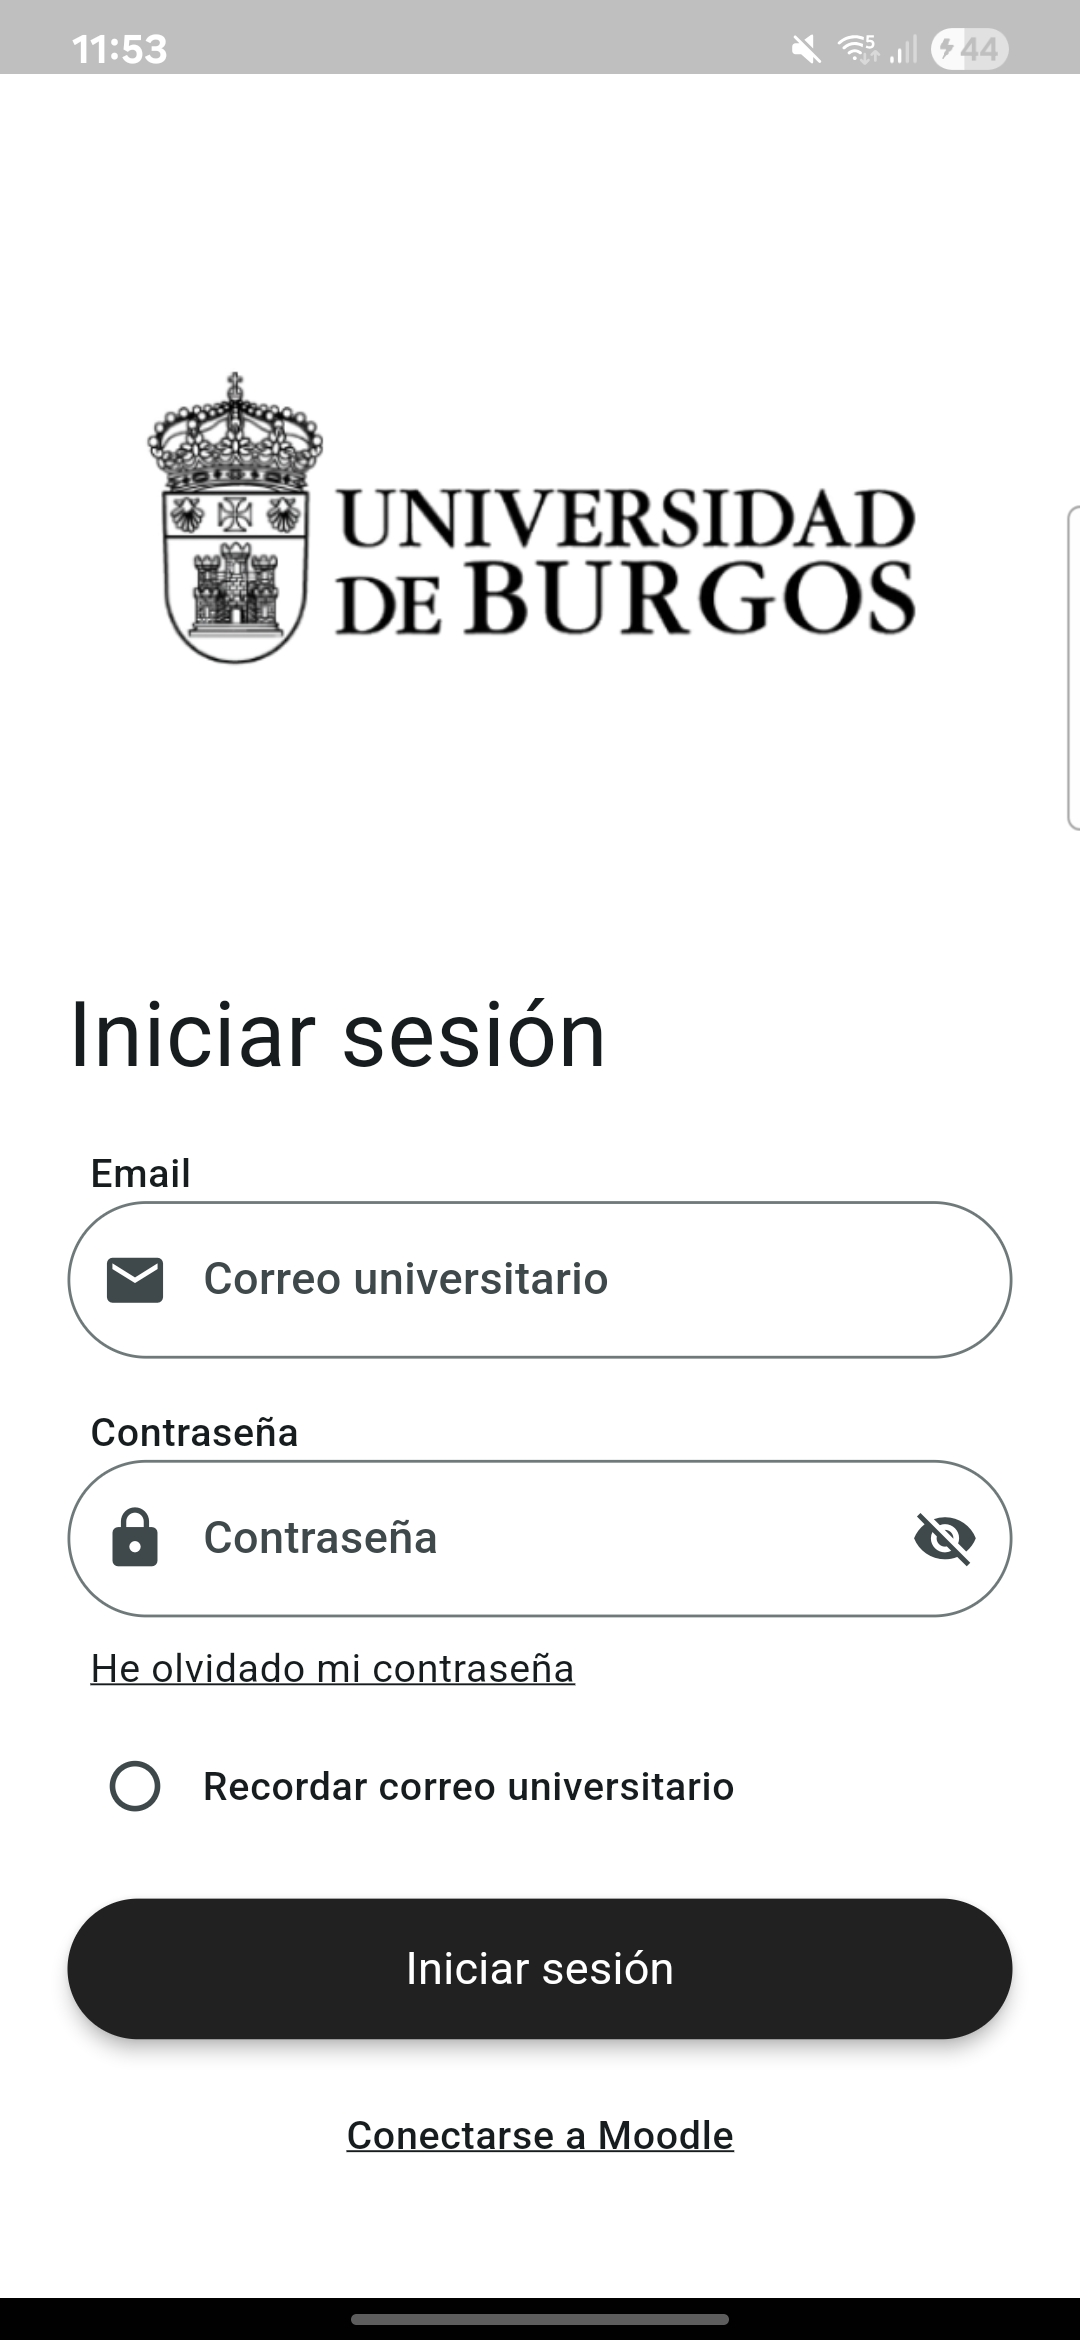
\includegraphics[width=0.4\linewidth]{img/inicio_sesion.jpg}
    \caption{Inicio de sesión de PlanLMS}
    \label{fig:inicio_sesion}
\end{figure}

En la figura \ref{fig:inicio_sesion} aparece el inicio de sesión que se compone de dos campos para introducir las credenciales de Moodle del usuario. Debajo hay un texto que redirige a la página de recuperaciónde contraseñas, en caso de no recordar la contraseña. Un \textit{checkbutton} que permite recordar el correo del usuario y el botón de acceso a la aplicación.

Por otra parte, esta el texto \textit{Conectarse a Moodle}. Al presionar dicho texto, se mostrará un pequeño diálogo, en el que se podrá introducir la \textit{URL} del servidor a conectar. Además, se incluye un sistema que verifica si la \textit{URL} introducida se trata de una plataforma Moodle.
\begin{figure}[H]
  \centering
  \begin{floatrow}
    \ffigbox
      {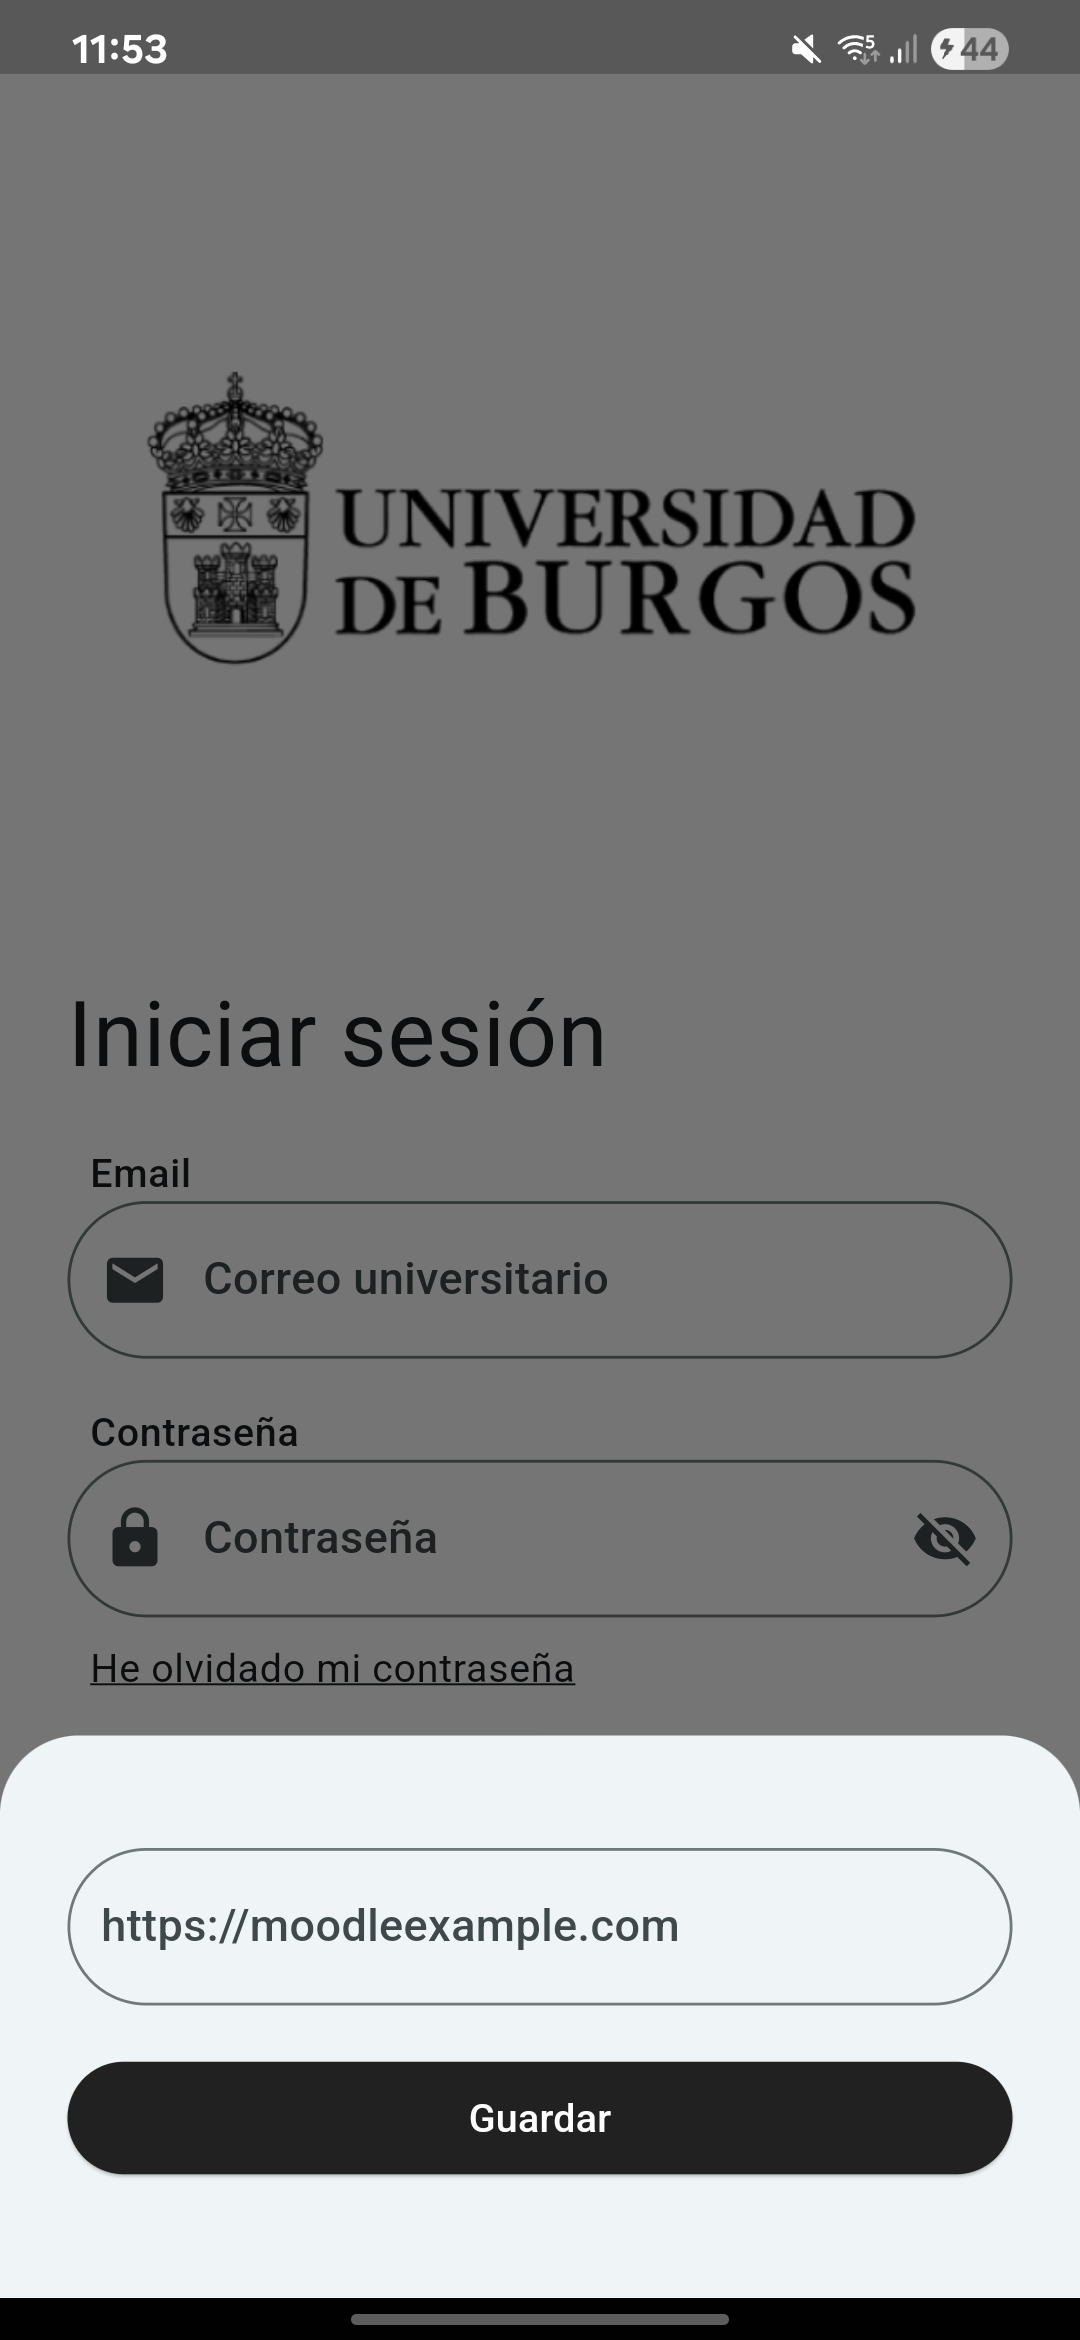
\includegraphics[width=0.5\linewidth]{img/conexion_moodle.jpg}}
      {\caption{Diálogo para conectarse a un Moodle}\label{fig:conexion_moodle}}
    \hfill
    \ffigbox
      {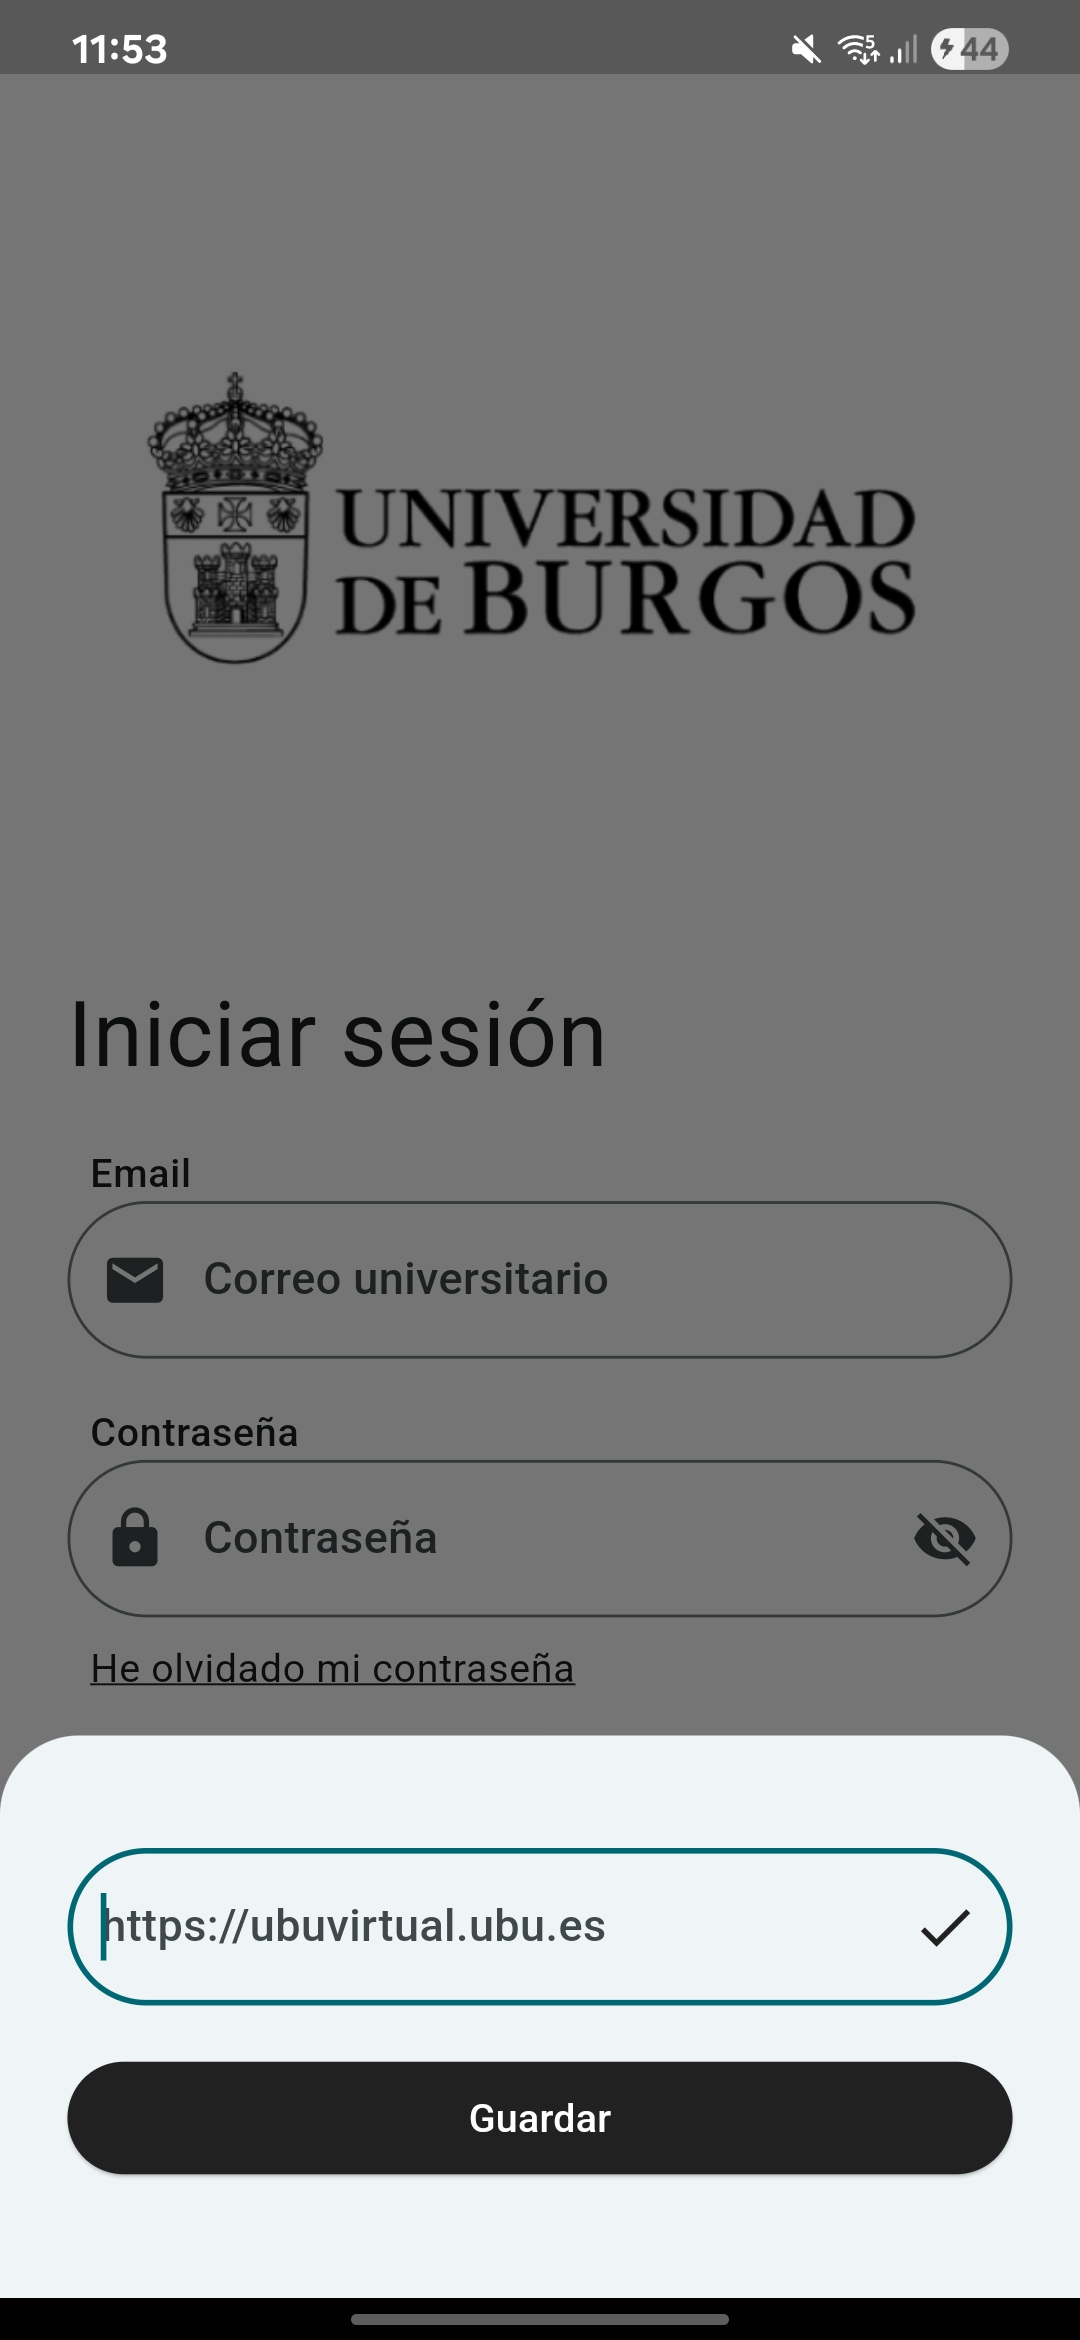
\includegraphics[width=0.5\linewidth]{img/conexion_ejemplo.jpg}}
      {\caption{Ejemplo de conexión}\label{fig:conexion_ejemplo}}
  \end{floatrow}
\end{figure}

Al presionar el botón \textit{Iniciar sesión}, se empezarán a obtener los siguientes datos de Moodle del usuario:
\begin{itemize}
    \item Información del usuario
    \item Cursos del usuario
    \item Tareas y cuestionarios de los cursos del usuario
   \item Entregas y calificaciones de las tareas y cuestionarios 
\end{itemize}
La duración del proceso de inicio de sesión puede variar en función de la cantidad de información que se vaya a extraer.

\subsection{Pantalla principal}
La primera pantalla que el usuario visualizará tras iniciar sesión, será la pantalla principal donde el usuario tendrá acceso a la siguientes funcionalidades de \textit{PlanLMS}:
\begin{itemize}
    \item Diagrama de Gantt
    \item Tareas personales
    \item Sistema de filtrado
\end{itemize}

Además, en la parte superior derecha hay un botón que se trata del cierre de sesión.
\begin{figure}[H]
    \centering
    
\includegraphics[width=0.4\linewidth]{img/pantalla_principal.jpg}
    \caption{Pantalla principal de PlanLMS}
    \label{fig:pantalla_principal}
\end{figure}

\subsection{Sistema de filtrado}
Para acceder a esta función basta con pulsar el botón situado en la esquina inferior derecha de la figura \ref{fig:pantalla_principal}. Al ser pulsado, aparecerá un diálogo en medio de la pantalla con todos los filtros disponibles. Algunos filtros solo afectan a algunas funcionalidades de la aplicación:
\begin{itemize}
    \item \textbf{Filtrado de cursos:} Diagrama de Gantt y Tareas Personales.
    \item \textbf{Filtrado de actividades:} Diagrama de Gantt.
    \item \textbf{Filtrado por fechas:} Diagrama de Gantt y Tareas Personales.
    \item \textbf{Filtrado por fechas disponibles:} Diagrama de Gantt.
\end{itemize}

\begin{figure}[H]
  \centering
  \begin{floatrow}
    \ffigbox
      {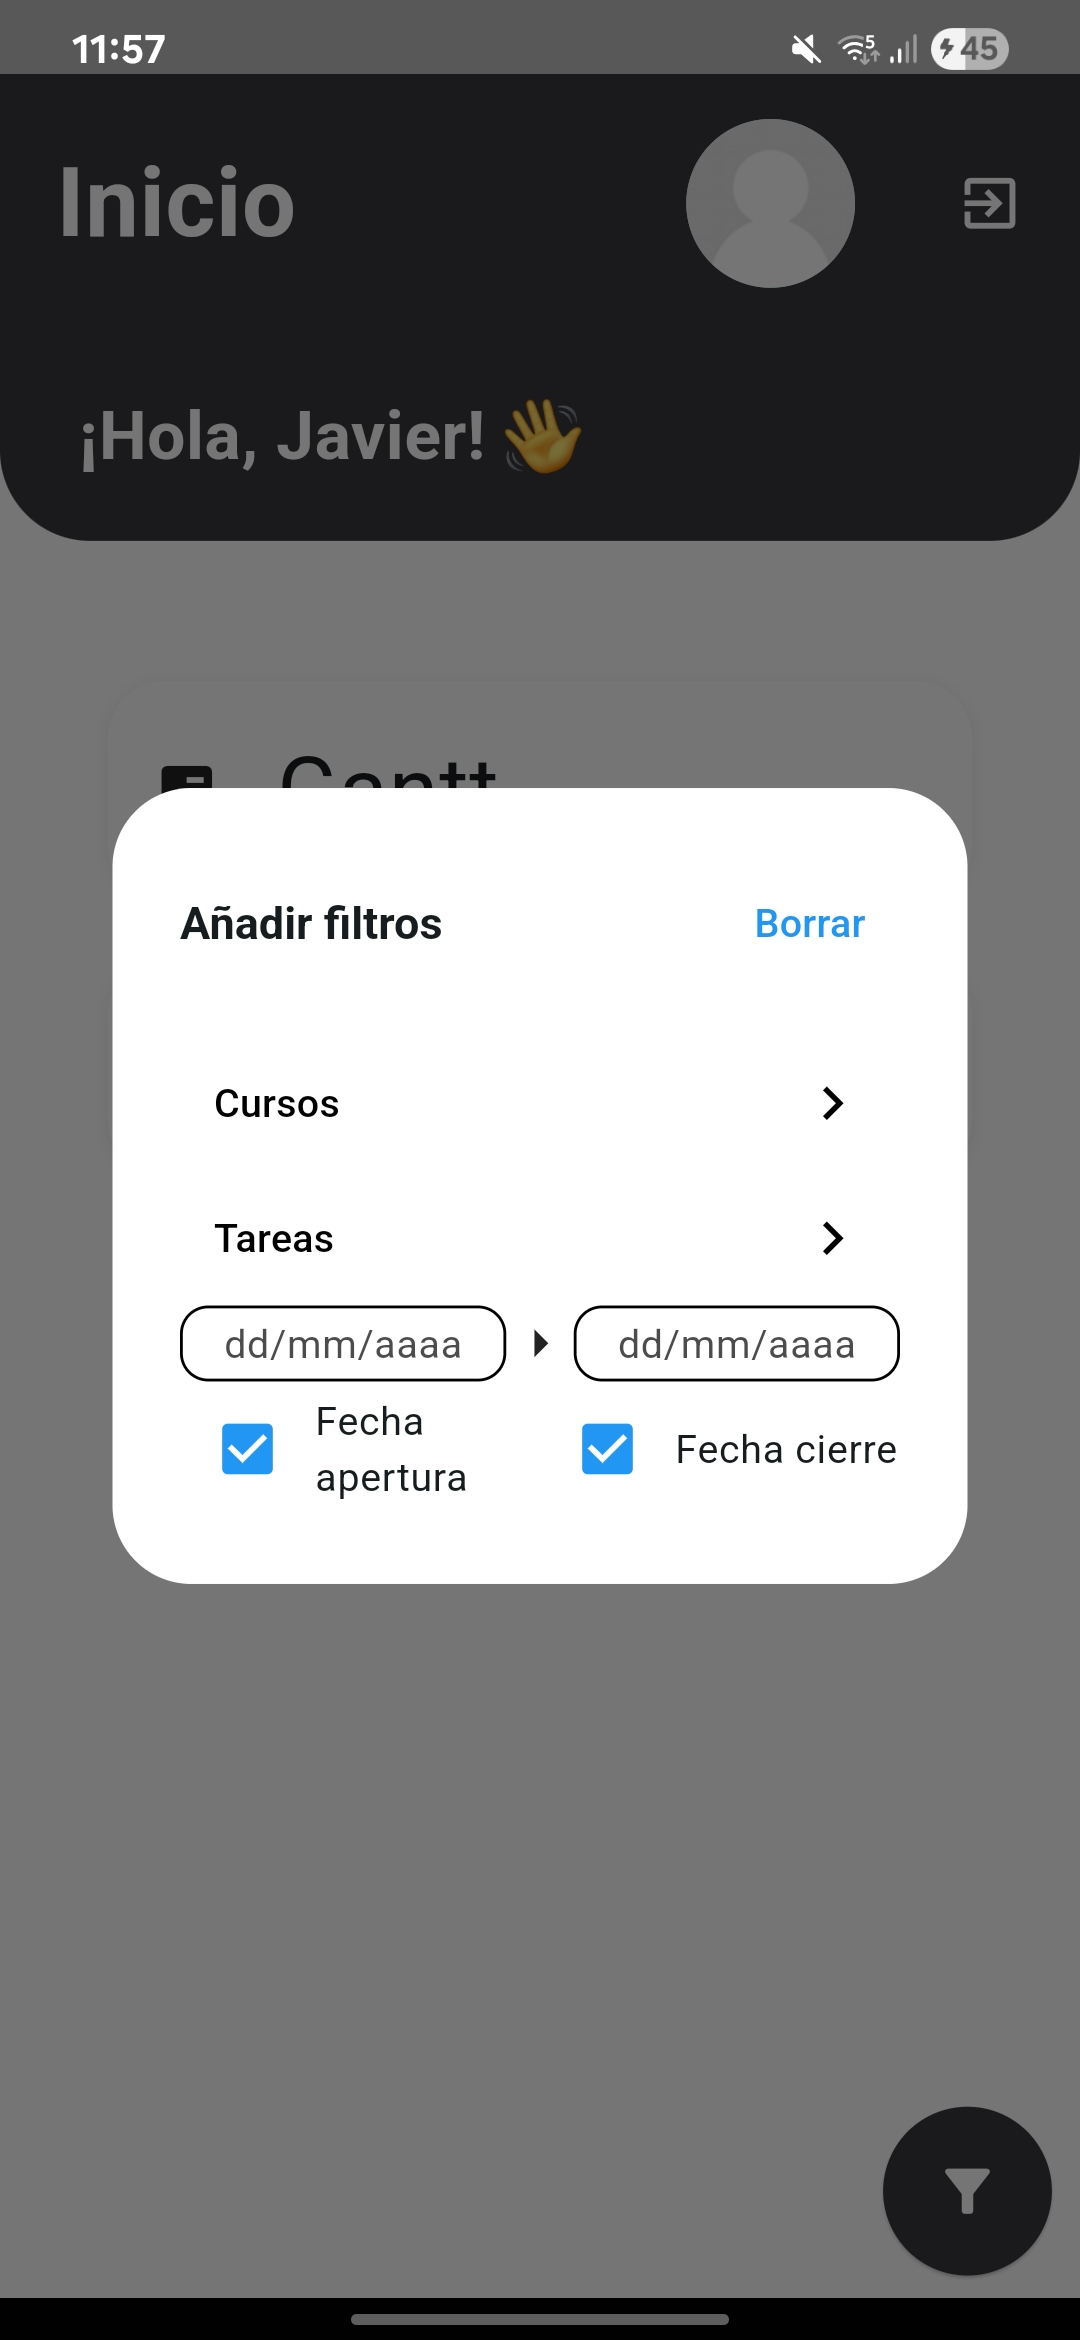
\includegraphics[width=0.5\linewidth]{img/filtros.jpg}}
      {\caption{Diálogo de filtros}\label{fig:filtros}}
    \hfill
    \ffigbox
      {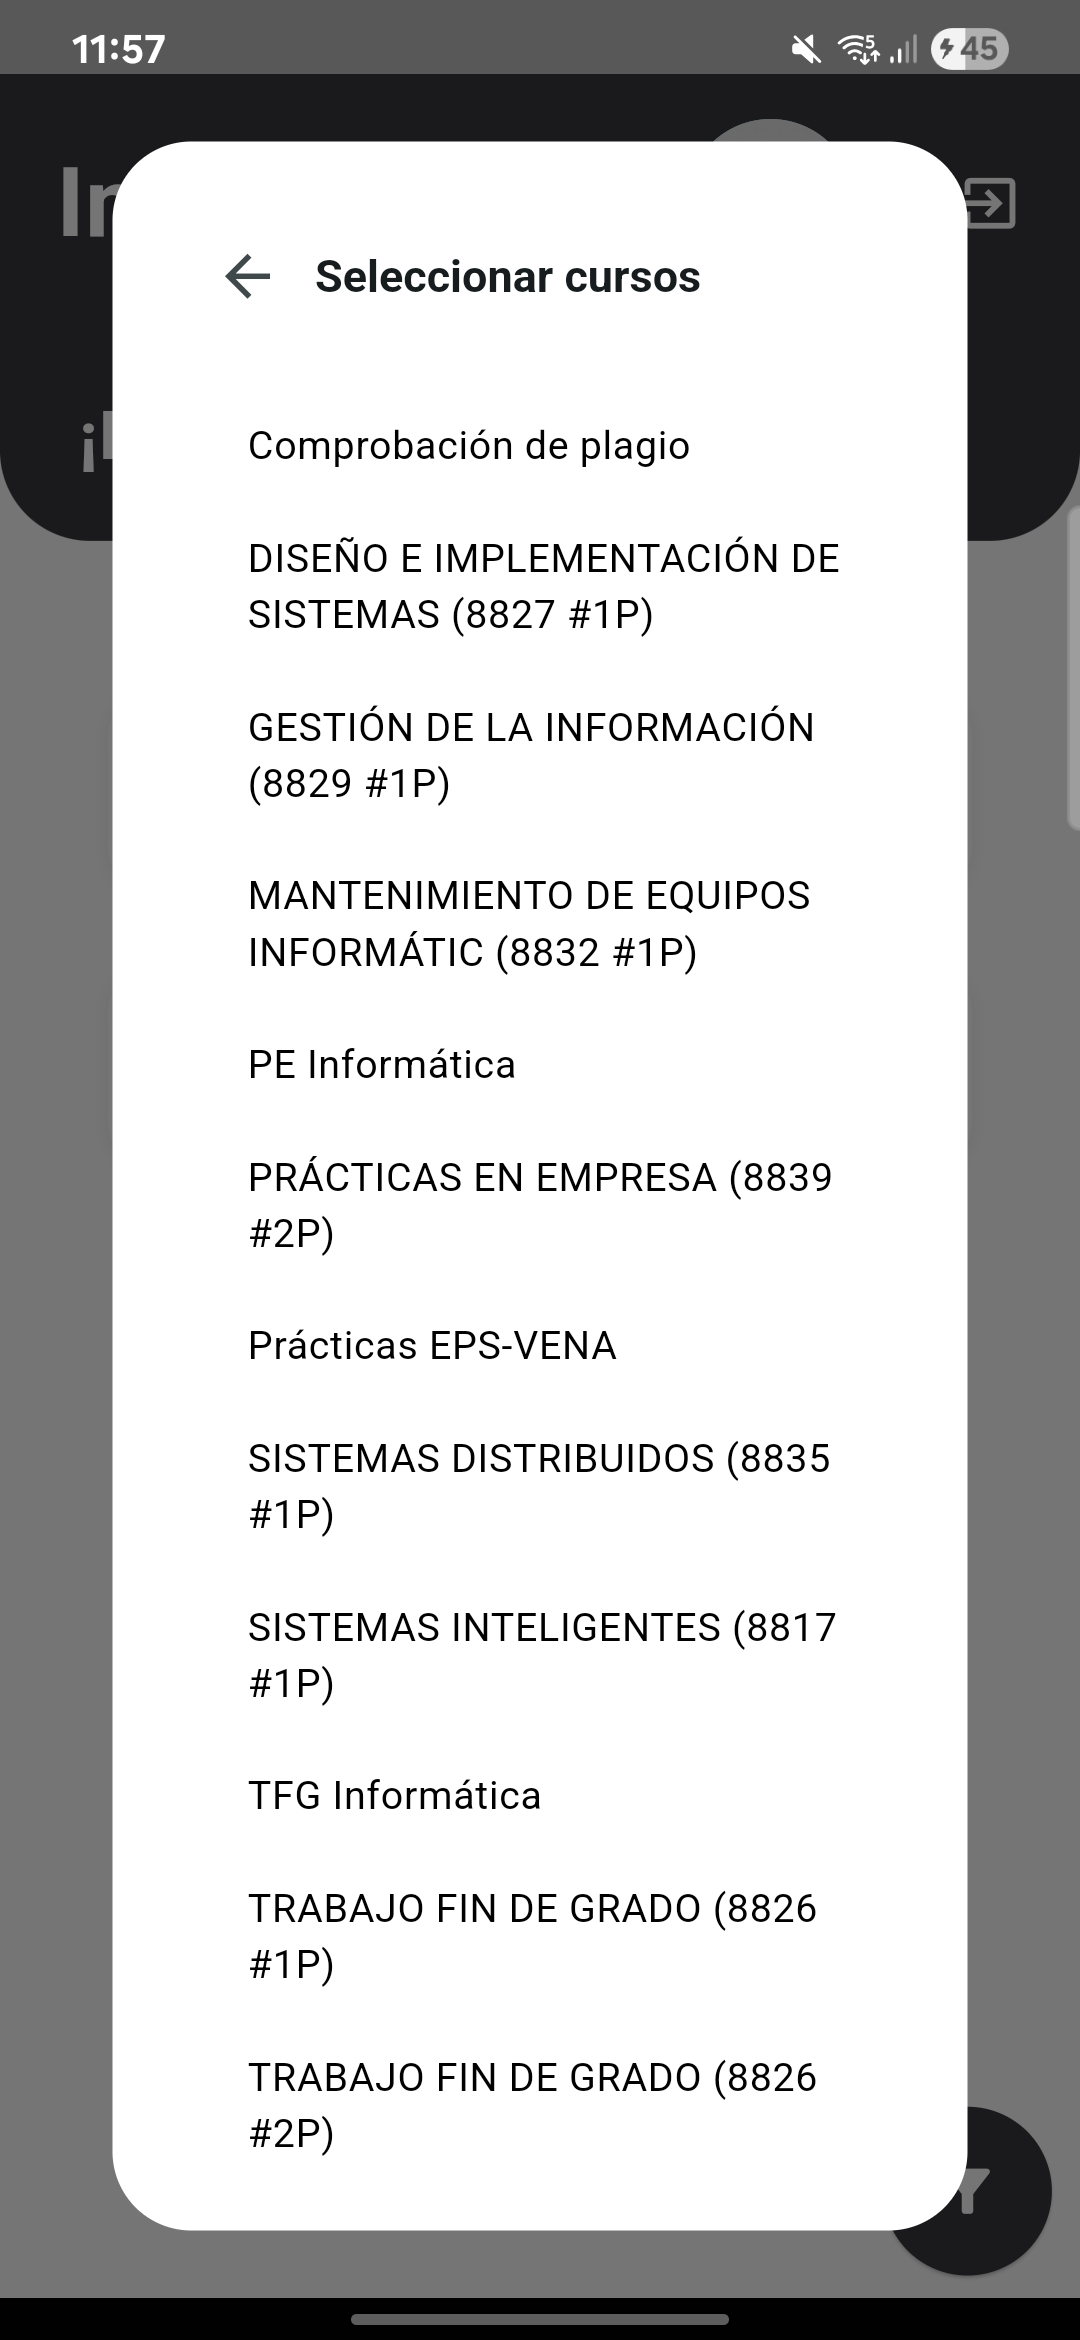
\includegraphics[width=0.5\linewidth]{img/filtros_cursos.jpg}}
      {\caption{Filtrado de cursos}\label{fig:filtros_cursos}}
  \end{floatrow}
\end{figure}
     
\begin{figure}[H]
    \centering
    {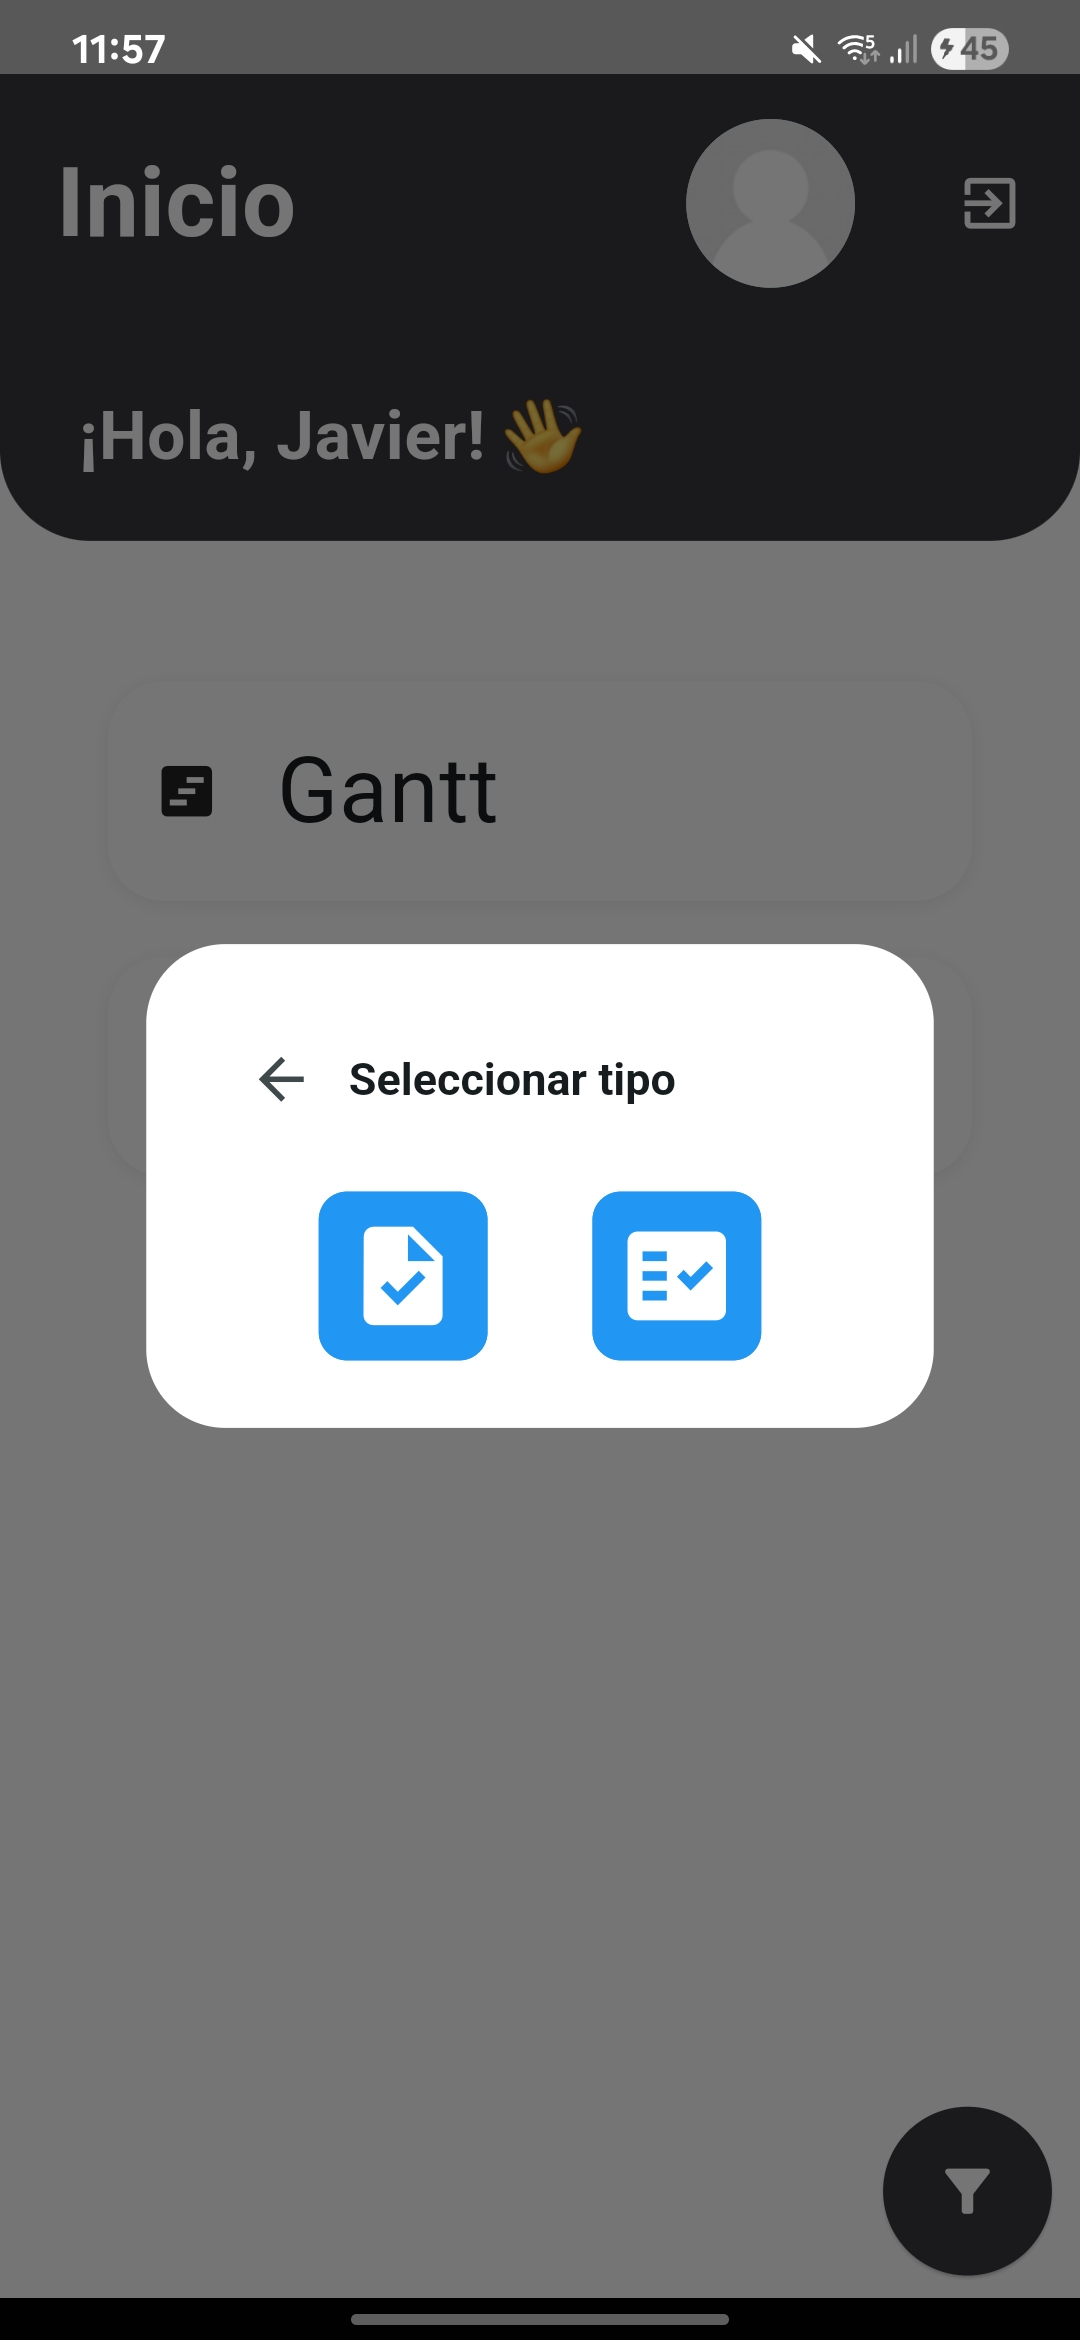
\includegraphics[width=0.25\linewidth]{img/filtros_actividades.jpg}}
     {\caption{Filtrado de actividades}
     \label{fig:filtros_actividades}}
\end{figure}

\subsubsection{Funcionamiento de los filtros}
A continuación se detalla el funcionamiento de cada uno de los filtros y como estos afectan a la aplicación.

\textbf{Filtrado de cursos}

Al acceder al diálogo \ref{fig:filtros_cursos}, se muestra una lista con todos los cursos del usuario. Por defecto, se filtrarían todos los cursos (aunque aparezcan como deseleccionados). Si se pulsa en el nombre de cada curso, este se marcaría y se filtrarían solo aquellos cursos que estén seleccionados.

\textbf{Filtrado de actividades}

Al acceder al diálogo \ref{fig:filtros_actividades}, se muestran dos iconos que por defecto se encuentran activados, por lo tanto, se filtrarían ambos tipos de actividades. En el caso de querer descartar alguna, basta con desmarcar la opción.

\textbf{Filtrado de fechas}

En el diálogo de filtros \ref{fig:filtros}, el tercer filtro disponible permite filtrar las fechas de tres formas diferentes:
\begin{itemize}
    \item Actividades a partir de una fecha
    \item Actividades anteriores a una fecha
    \item Actividades entre dos fechas
\end{itemize}


\textbf{Filtrado de fechas disponibles}

El último filtro permite filtrar aquellas actividades que por configuración carecen de fecha de apertura o de cierre, o incluso ambas. Consiste en dos casillas que en función de si están marcadas o no, mostrarán actividades con la disponibilidad de esas fechas.

\subsubsection{Diagrama de Gantt}
Una de las pantallas a las que se puede acceder desde la \textit{Pantalla Principal} \ref{fig:pantalla_principal} es el diagrama de Gantt. Esta pantalla permite al usuario visualizar las actividades filtradas en un diagrama de Gantt, que además puede ser personalizado con filtros para modificar su apariencia.
\begin{figure}[H]
  \centering
  \begin{floatrow}
    \ffigbox
      {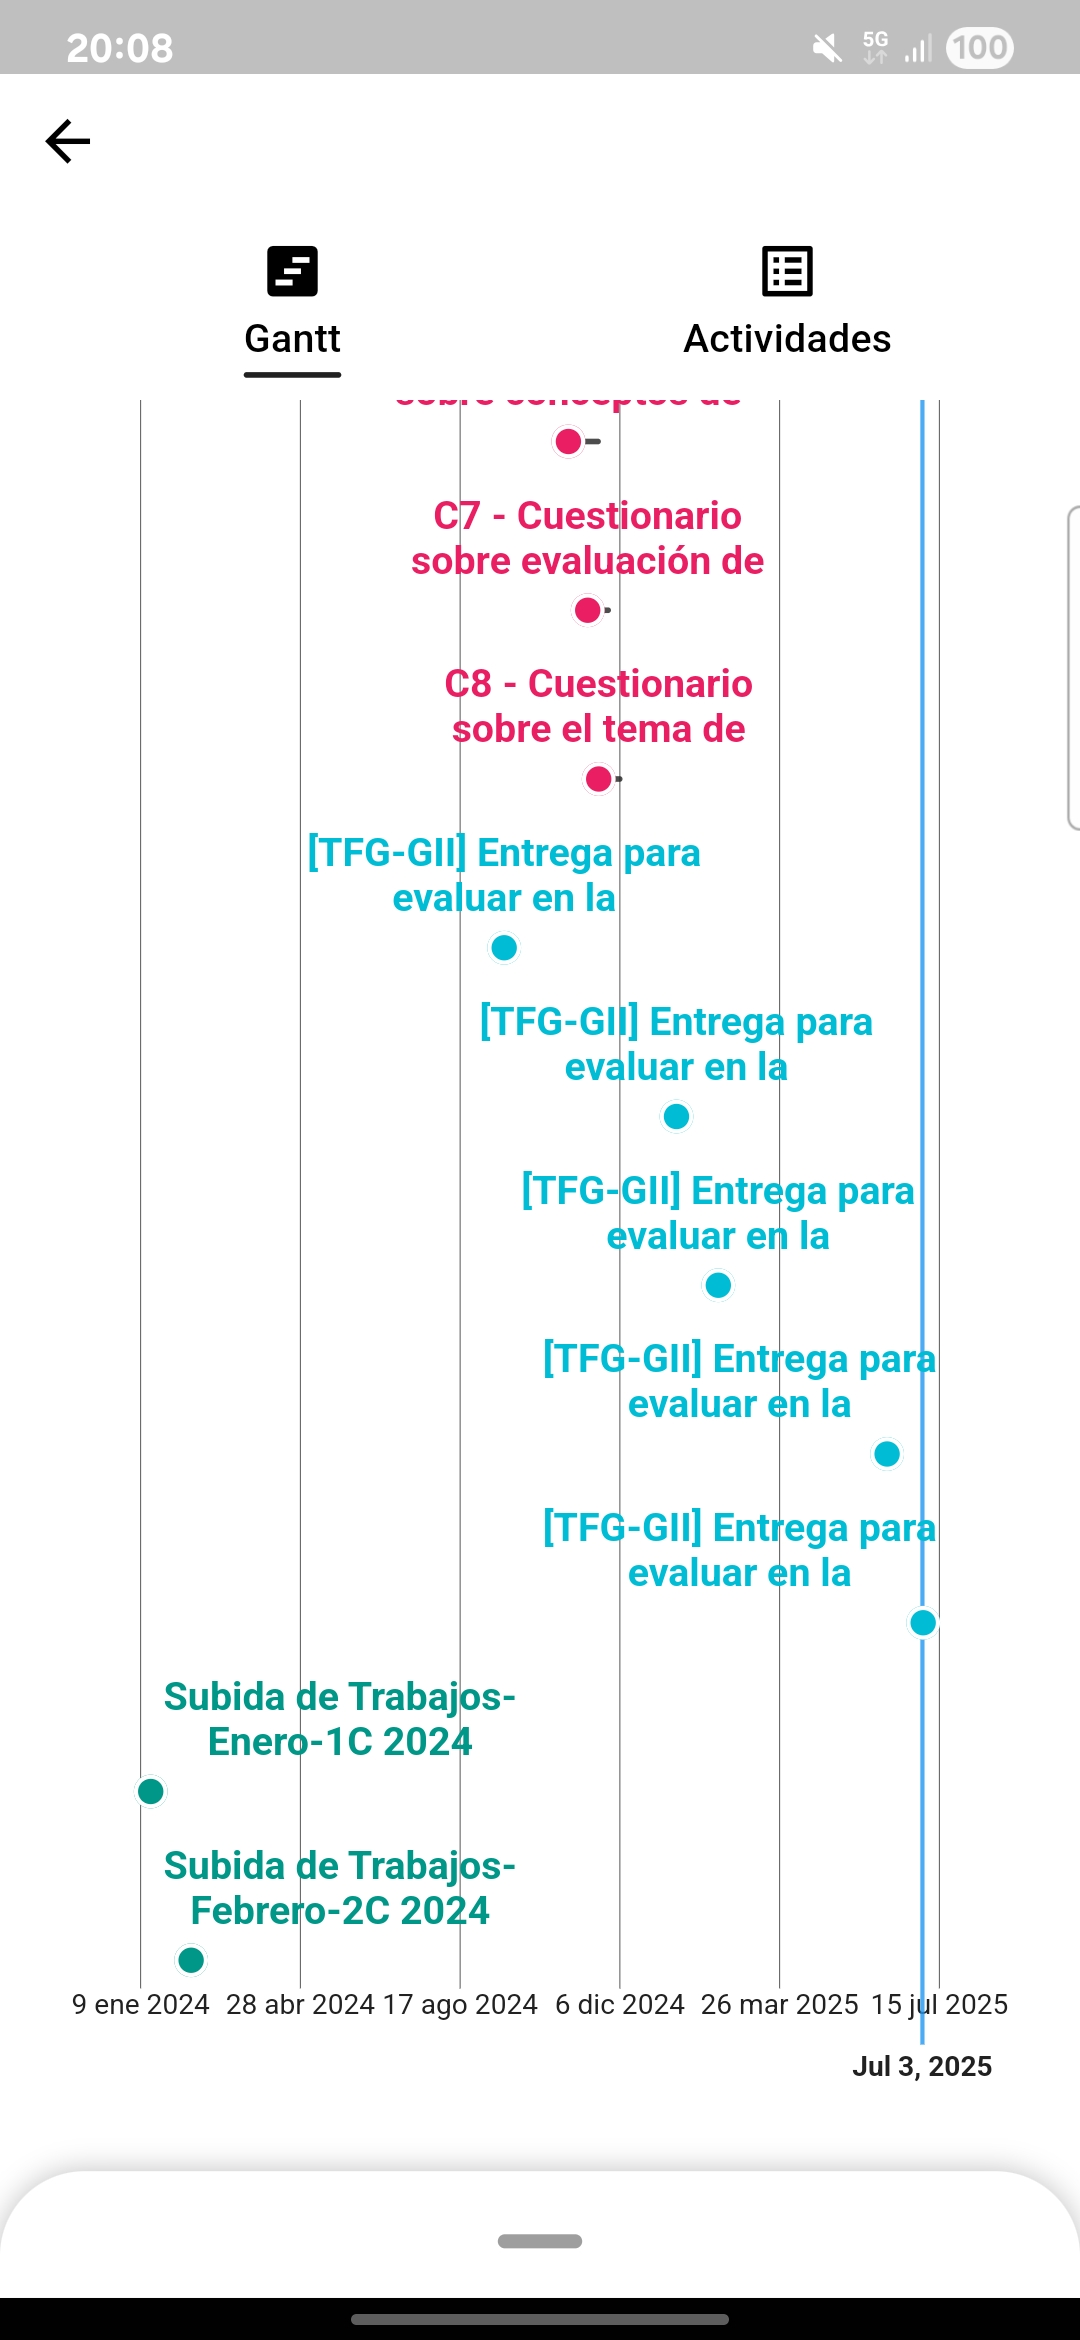
\includegraphics[width=0.5\linewidth]{img/diagrama_gantt.jpg}}
      {\caption{Pantalla de diagrama de Gantt}\label{fig:diagrama_gantt}}
    \hfill
    \ffigbox
     {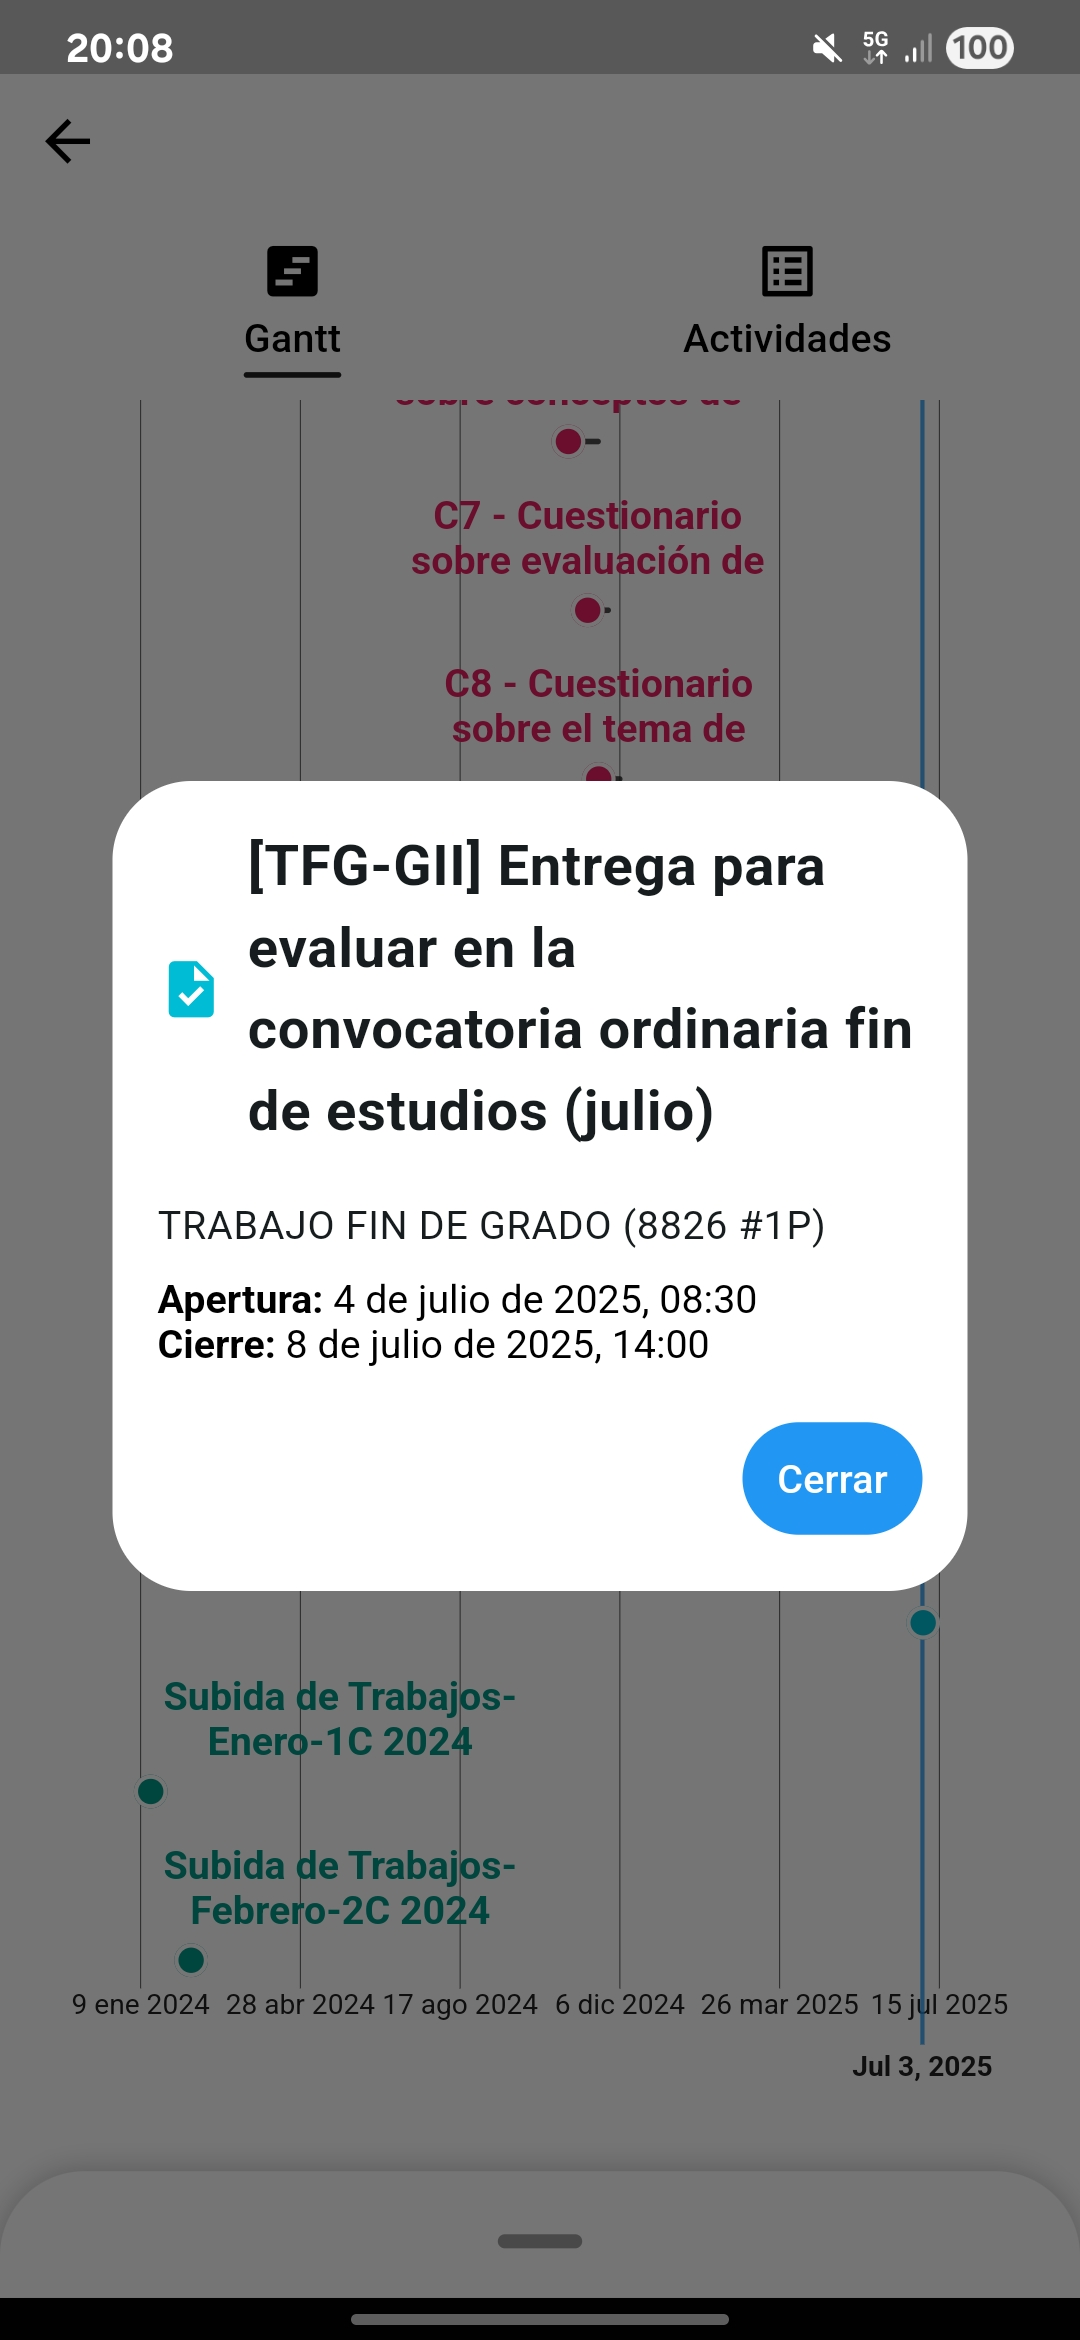
\includegraphics[width=0.5\linewidth]{img/gantt_actividad.jpg}}
     {\caption{Diálogo de actividad en diagrama de Gantt}
     \label{fig:gantt_actividad}}
  \end{floatrow}
\end{figure}

Si se presiona cualquier punto de los que aparecen en el diagrama, se abrirá un pequeño diálogo con información de la actividad \ref{fig:gantt_actividad}.

En la parte inferior de la pantalla \ref{fig:diagrama_gantt}
se puede observar un pequeño panel que si es deslizado hacia arriba, mostrará dos filtros que permiten modificar la estética del diagrama.
\begin{figure}[H]
  \centering
  \begin{floatrow}
    \ffigbox
      {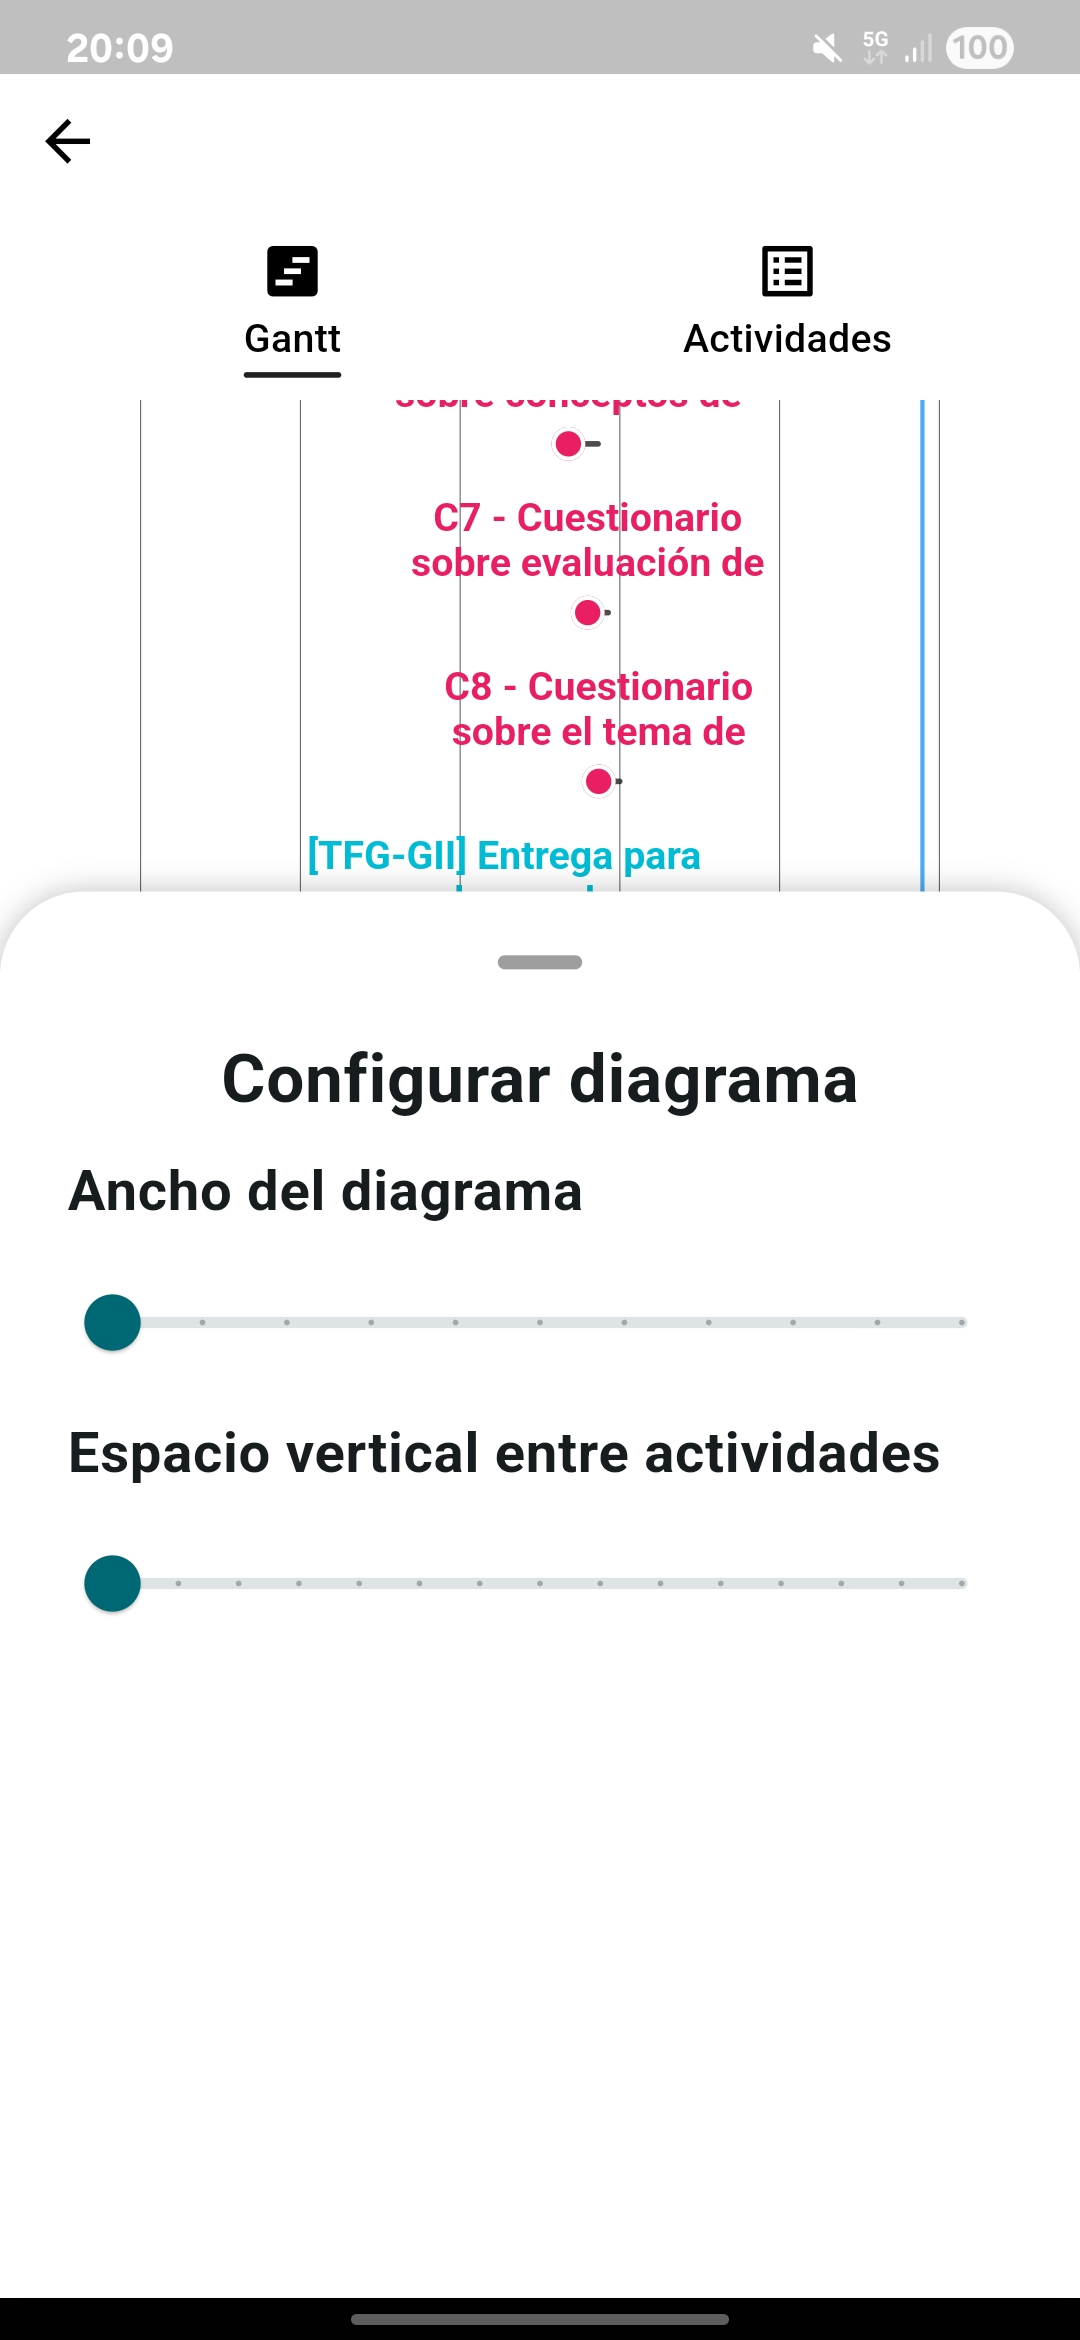
\includegraphics[width=0.5\linewidth]{img/filtros_diagrama.jpg}}
      {\caption{Filtros del diagrama de Gantt}
      \label{fig:filtros_diagrama}}
    \hfill
    \ffigbox
     {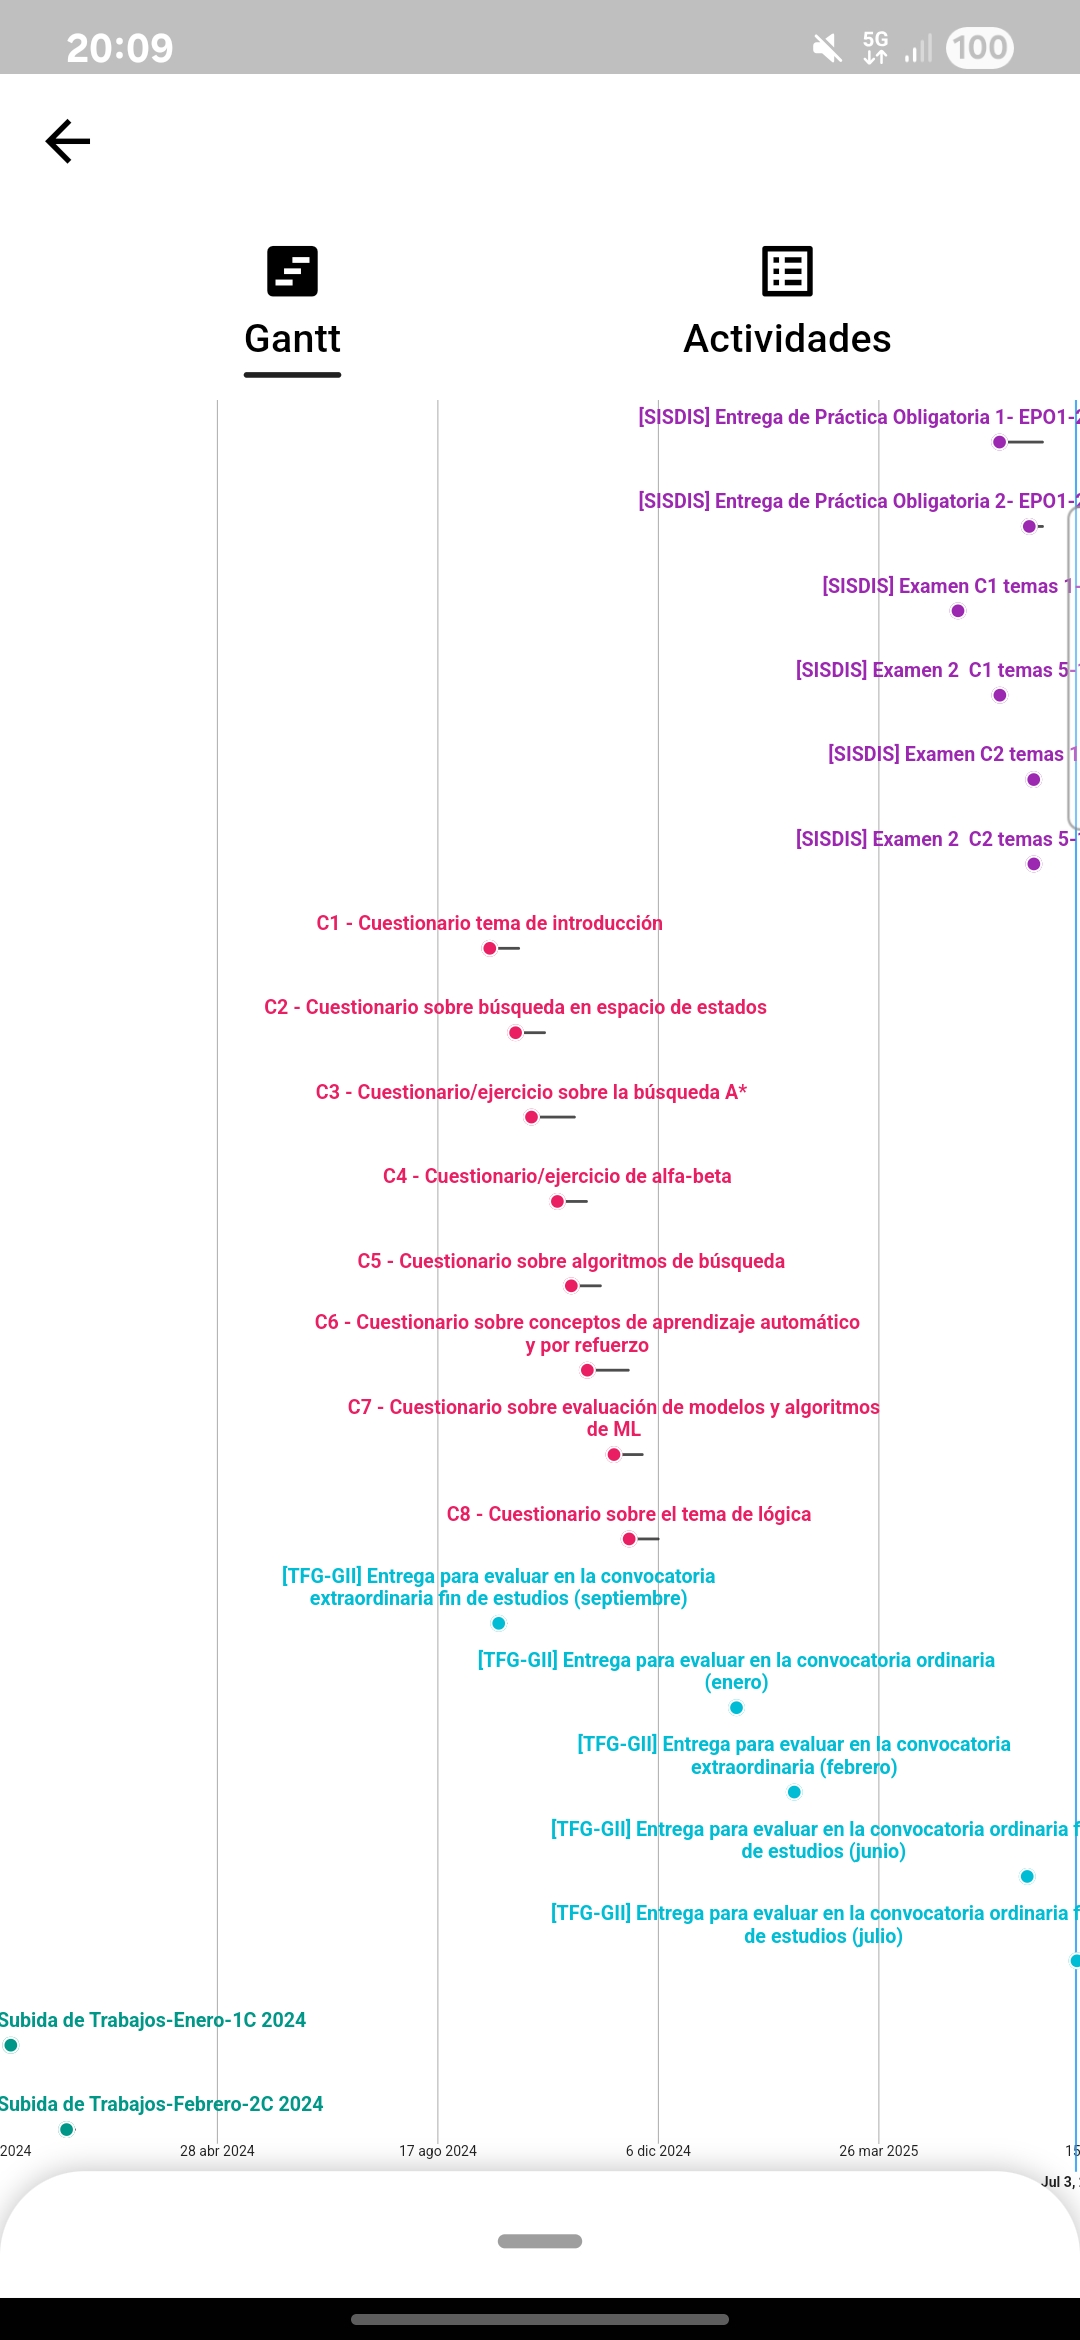
\includegraphics[width=0.5\linewidth]{img/diagrama_filtrado.jpg}}
     {\caption{Filtros estéticos aplicados sobre el diagrama}
     \label{fig:diagrama_filtrado}}
  \end{floatrow}
\end{figure}

Otra funcionalidad del diagrama, es que permite el desplazamiento en todas las direcciones, así como hacer \textit{zoom}, todo mediante gestos en la pantalla con los dedos.

Por otra parte, dentro de la pantalla del diagrama de Gantt, hay una sección de actividades \ref{fig:tareas_gantt}, en la cual aparecen todas las actividades que se encuentren dibujadas en el diagrama de Gantt.
\begin{figure}[H]
    \centering
    {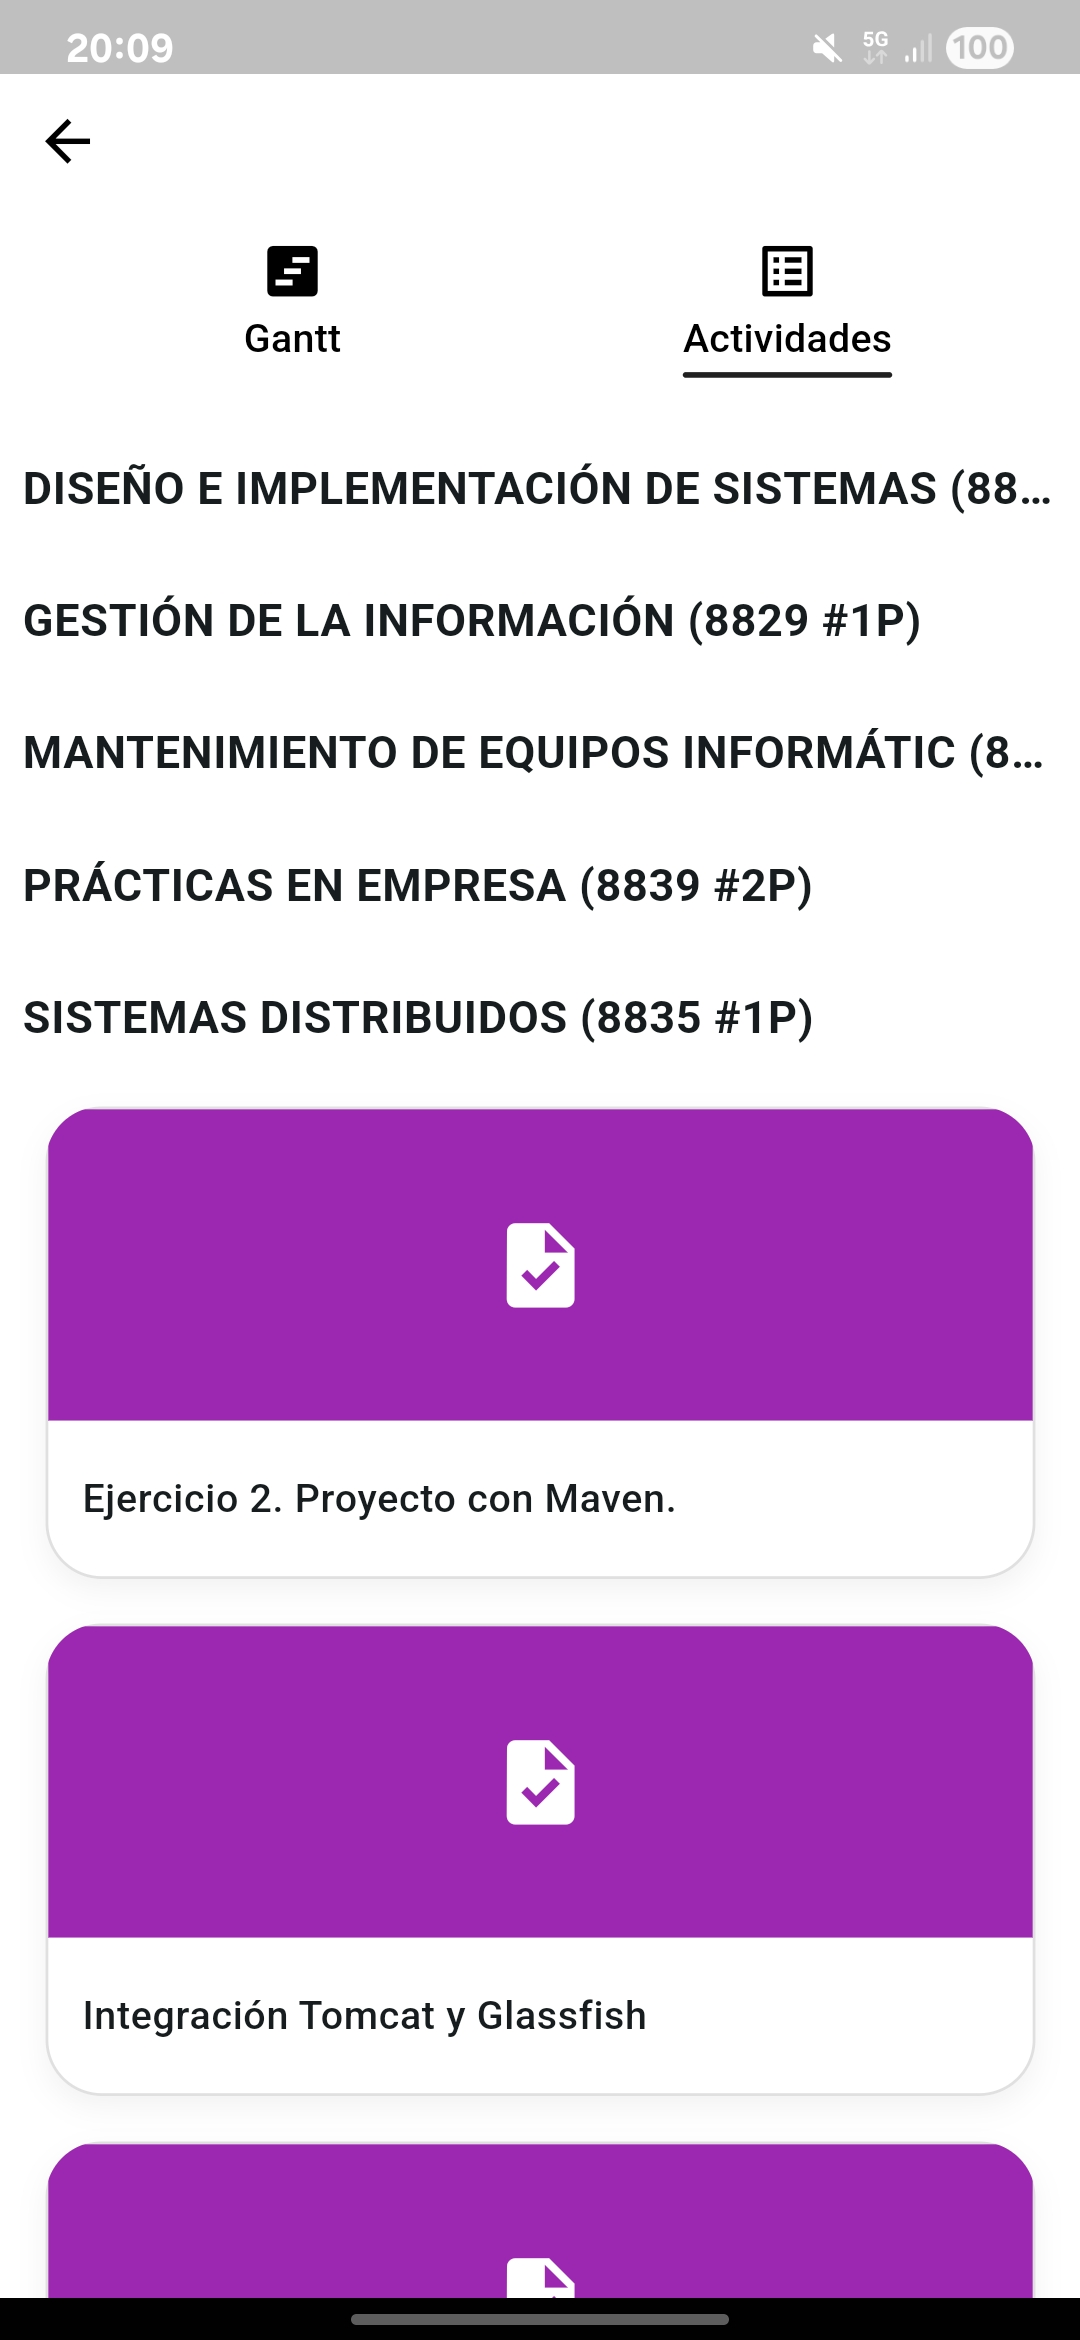
\includegraphics[width=0.25\linewidth]{img/tareas_gantt.jpg}}
    {\caption{Sección de actividades del diagrama de Gantt}
    \label{fig:tareas_gantt}}
\end{figure}

Al presionar una de las tarjetas que aparecen, se despliega una nueva ventana \ref{fig:tarea_gantt} con toda la información que se recoge de Moodle y que pueda llegar a ser útil para el usuario.
\begin{figure}[H]
    \centering
    {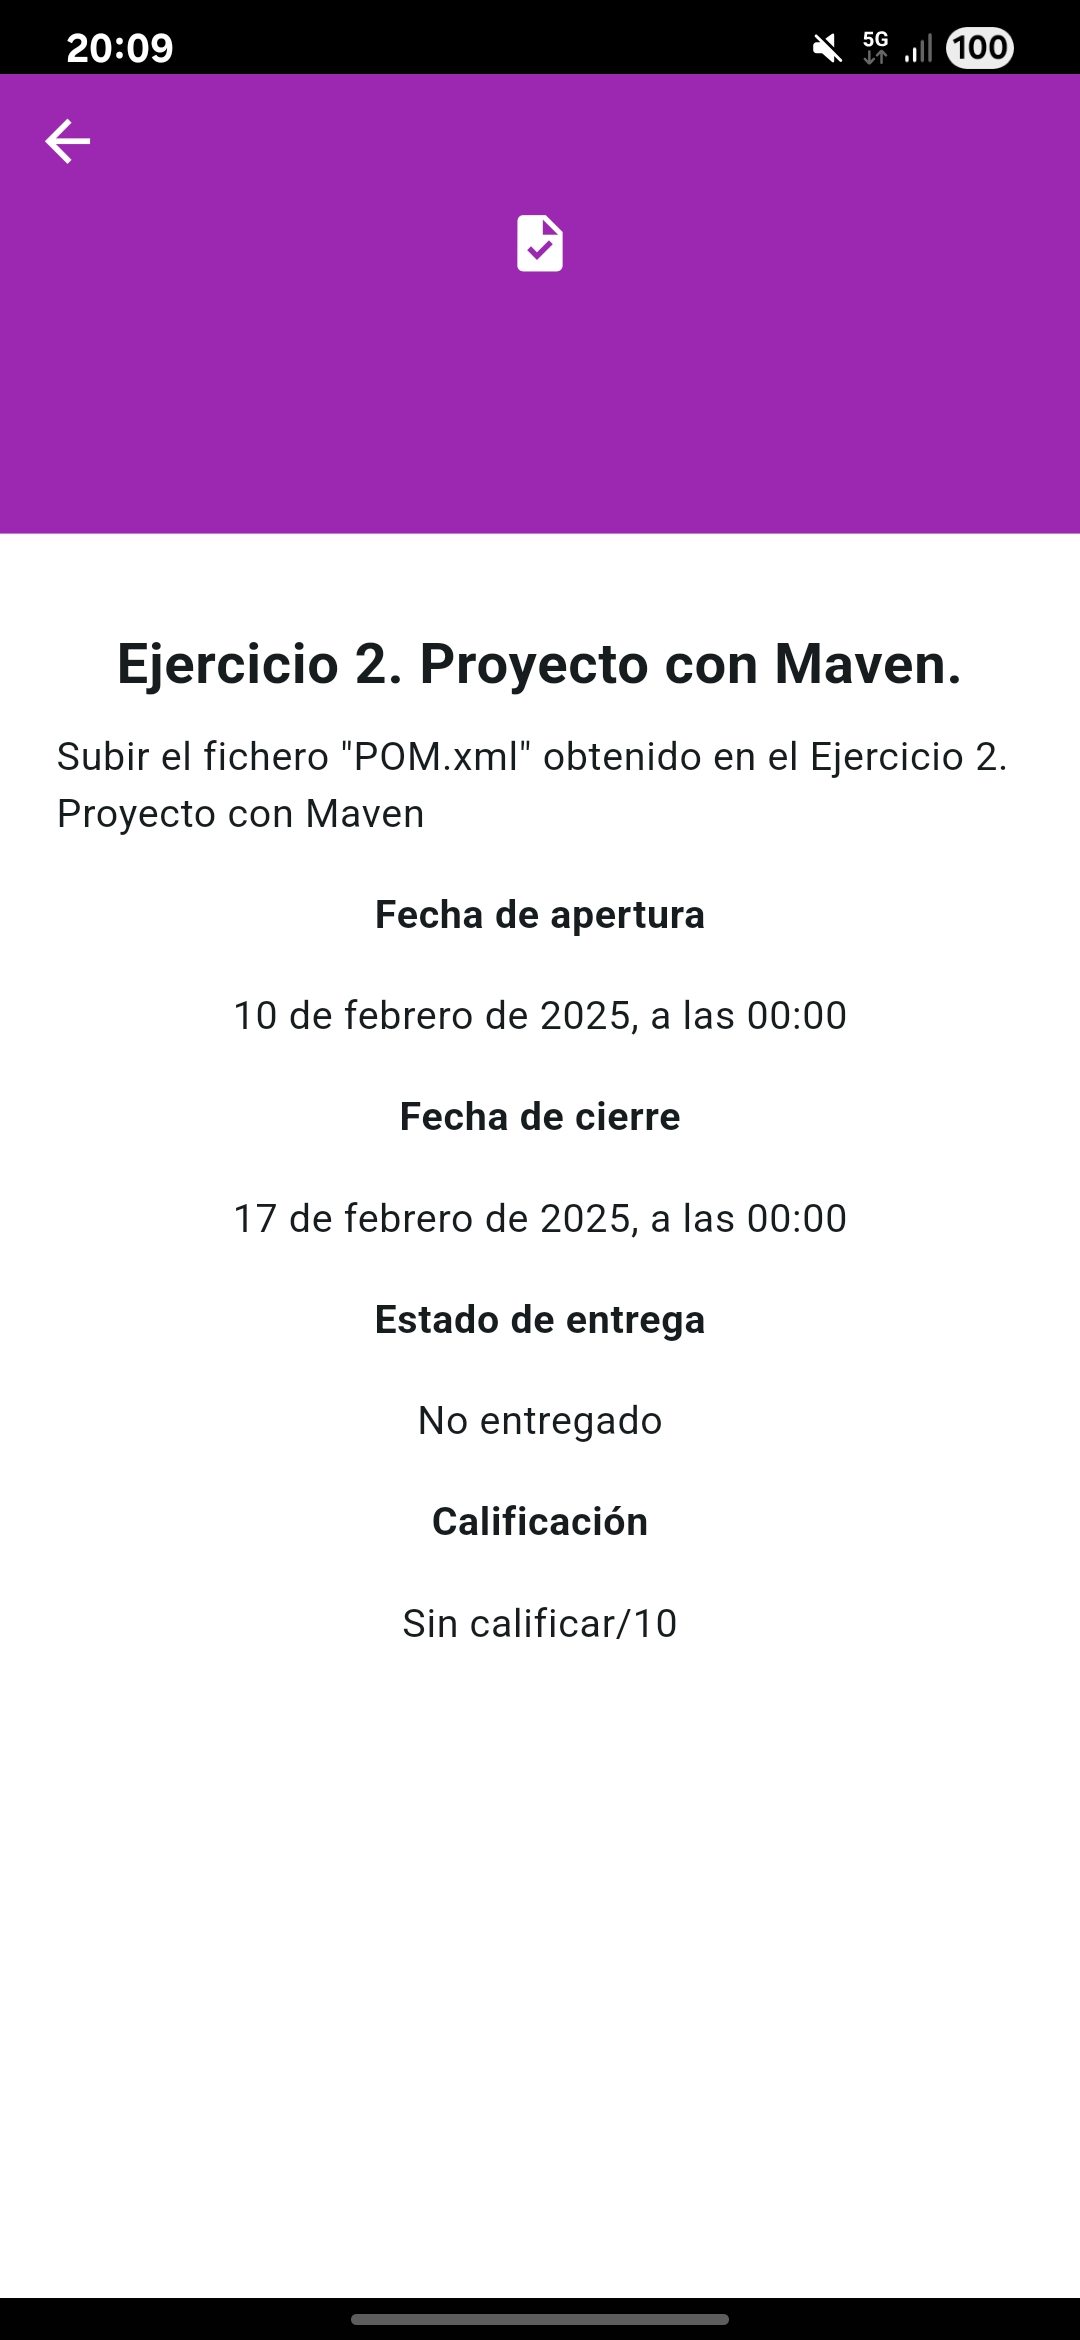
\includegraphics[width=0.25\linewidth]{img/tarea_gantt.jpg}}
     {\caption{Ventana con información de la actividad}
     \label{fig:tarea_gantt}}
\end{figure}

\subsubsection{Tareas Personales}
La última funcionalidad a explicar, son la tareas personales. Esta función tiene acceso desde la pantalla principal \ref{fig:pantalla_principal} y permite al usuario crear sus propias tareas personales con información personalizada.

Dentro de esta pantalla existen dos secciones: \textit{Pendientes} y \textit{Completadas}. Como su propio nombre indica, hacen referencia al estado de finalización de la tarea. A su vez, dentro de cada sección hay distintas subsecciones:
\begin{itemize}
    \item \textbf{Pendientes:} Hoy, Mañana, Esta Semana y Todos
    \item \textbf{Completadas:} Hoy, Últimos 7d, Este mes y Todos
\end{itemize}
\begin{figure}[H]
  \centering
  \begin{floatrow}
    \ffigbox
      {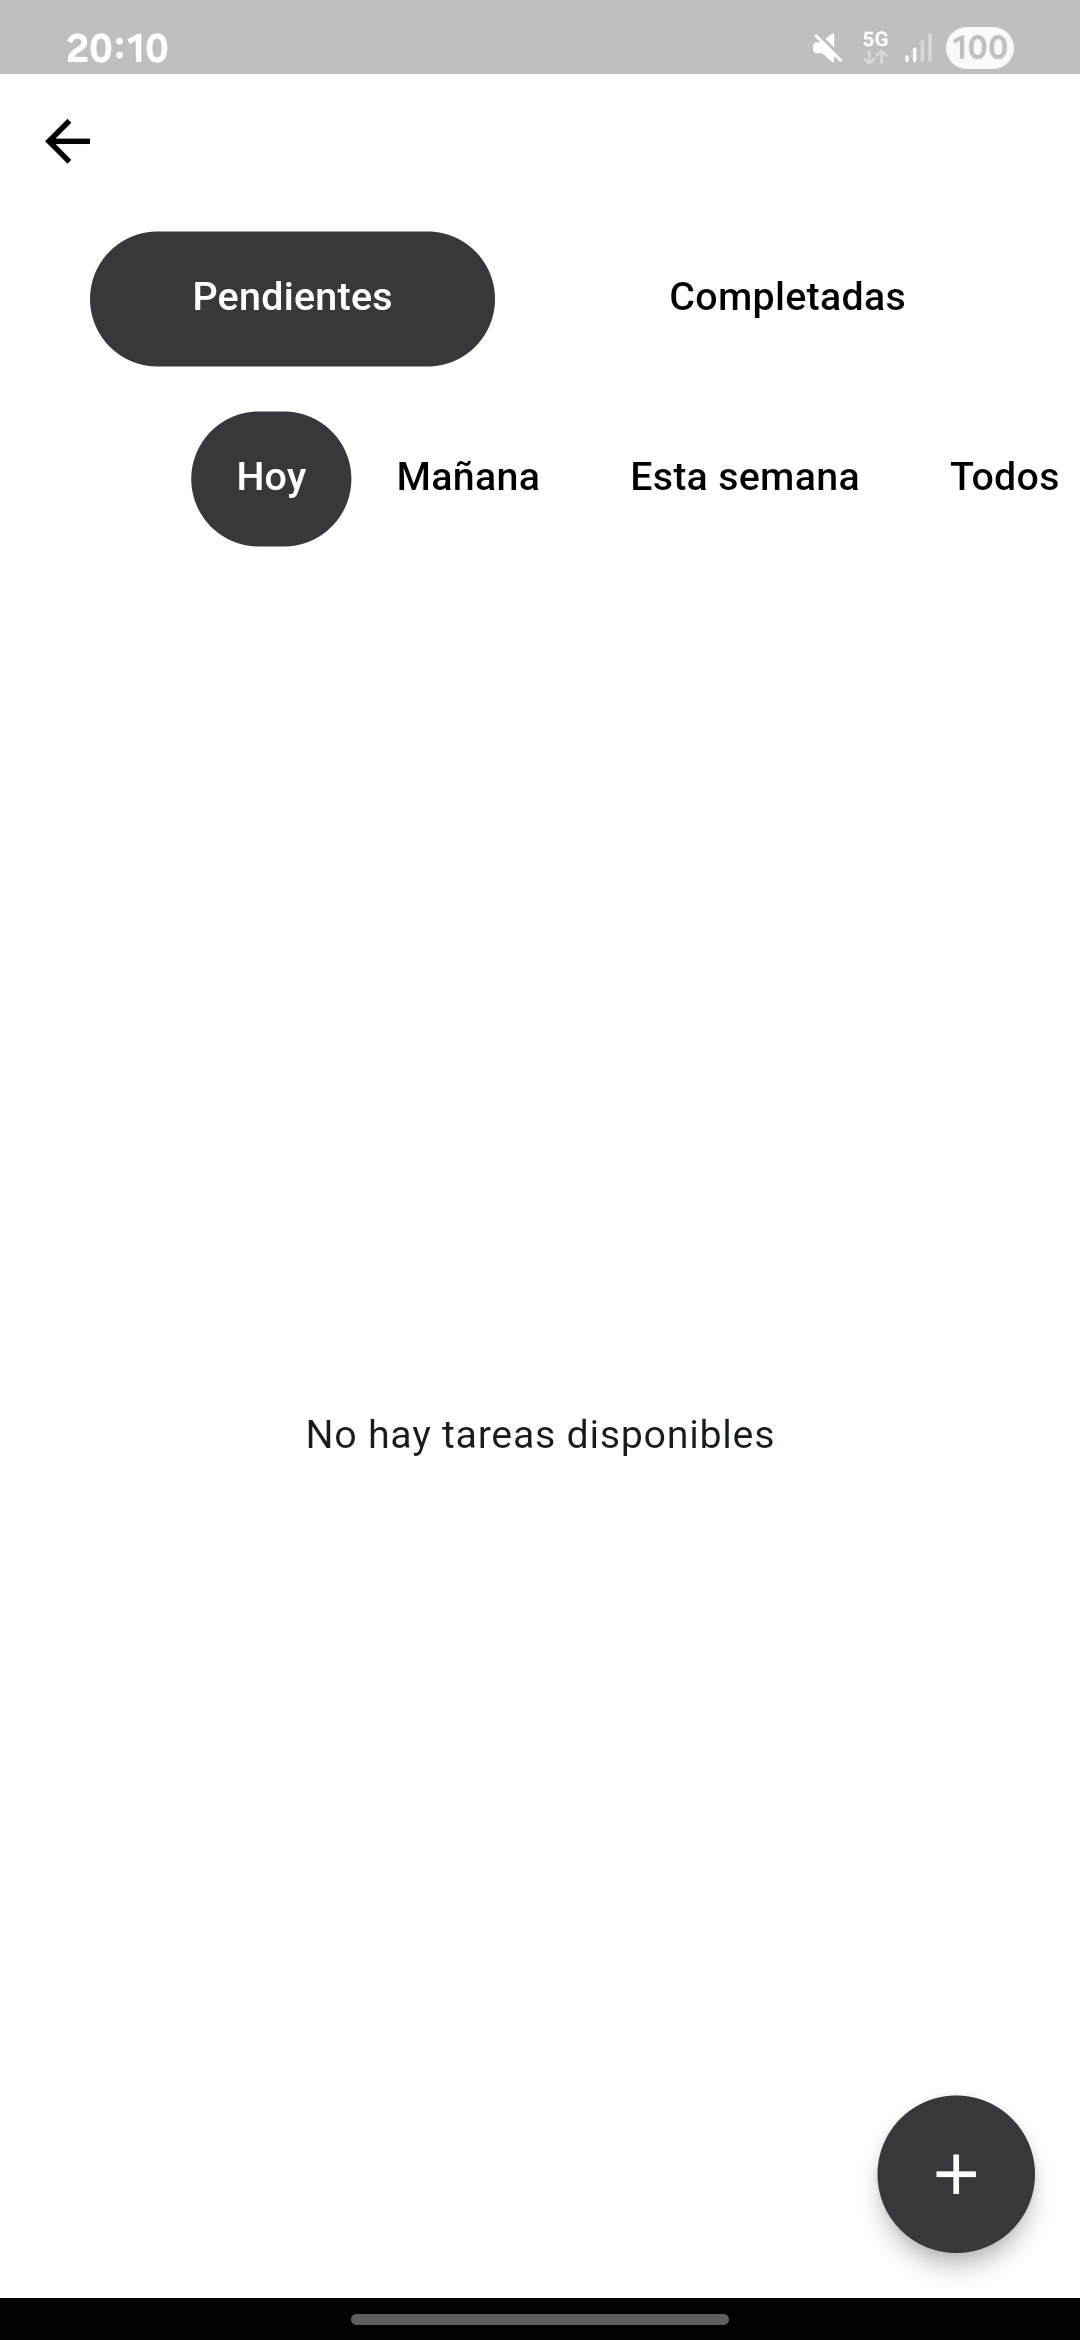
\includegraphics[width=0.5\linewidth]{img/tareas_personales_pendientes.jpg}}
      {\caption{Sección de tareas pendientes}
      \label{fig:tareas_personales_pendientes}}
    \hfill
    \ffigbox
     {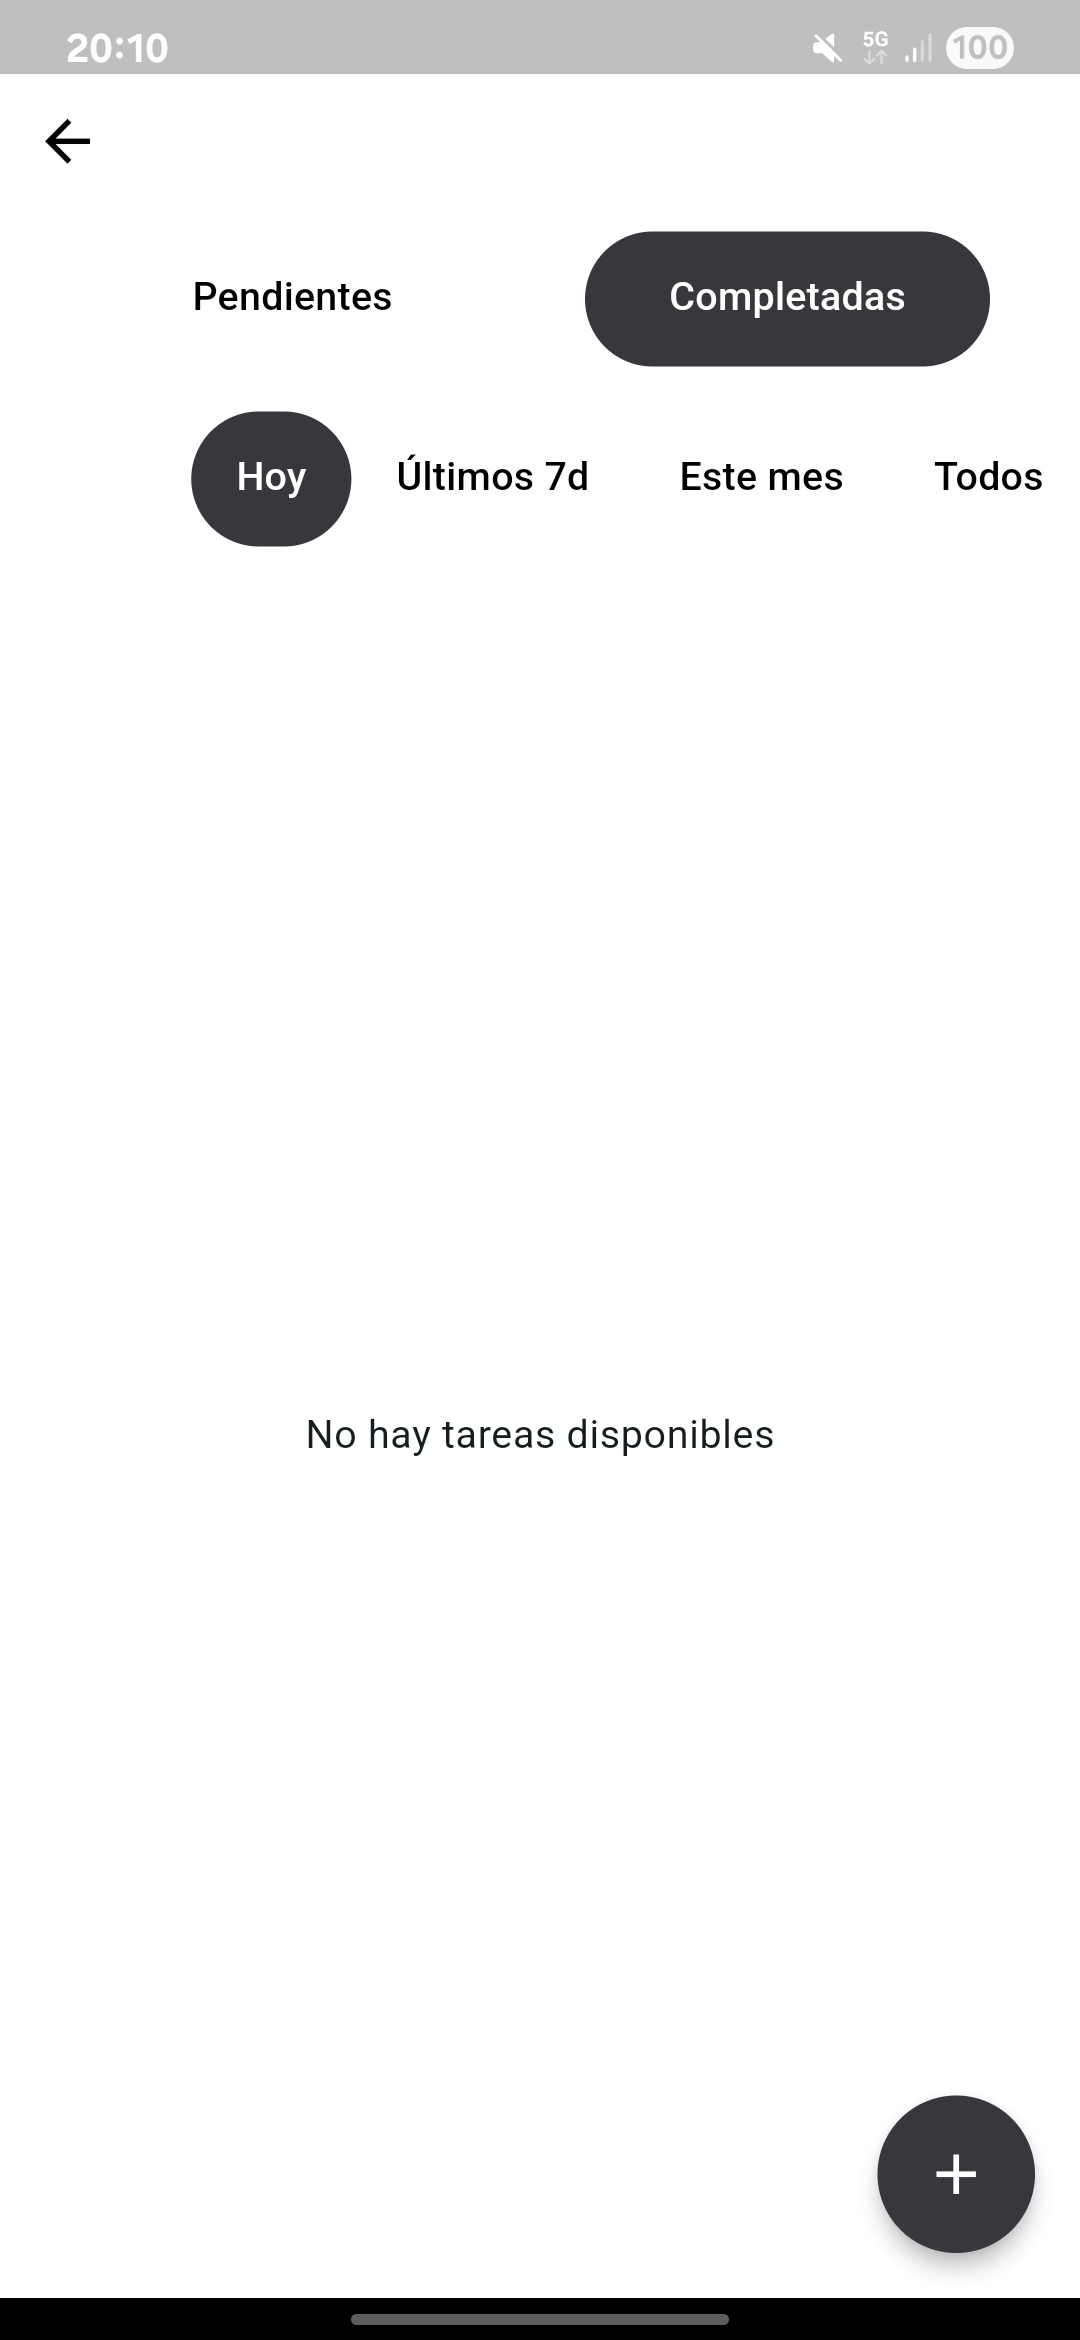
\includegraphics[width=0.5\linewidth]{img/tareas_personales_completadas.jpg}}
     {\caption{Sección de tareas completadas}
     \label{fig:tareas_personales_completadas}}
  \end{floatrow}
\end{figure}

En la parte inferior derecha de la pantalla \ref{fig:tareas_personales_pendientes} se encuentra un botón que al ser pulsado abre una ventana con un formulario de \textit{Creación de tareas}. El cual consta de unos campos obligatorios y otros opcionales. Una vez rellenados los campos y guardada la tarea, esta se añade directamente a la sección de tareas pendientes.
\begin{figure}[H]
  \centering
  \begin{floatrow}
    \ffigbox
      {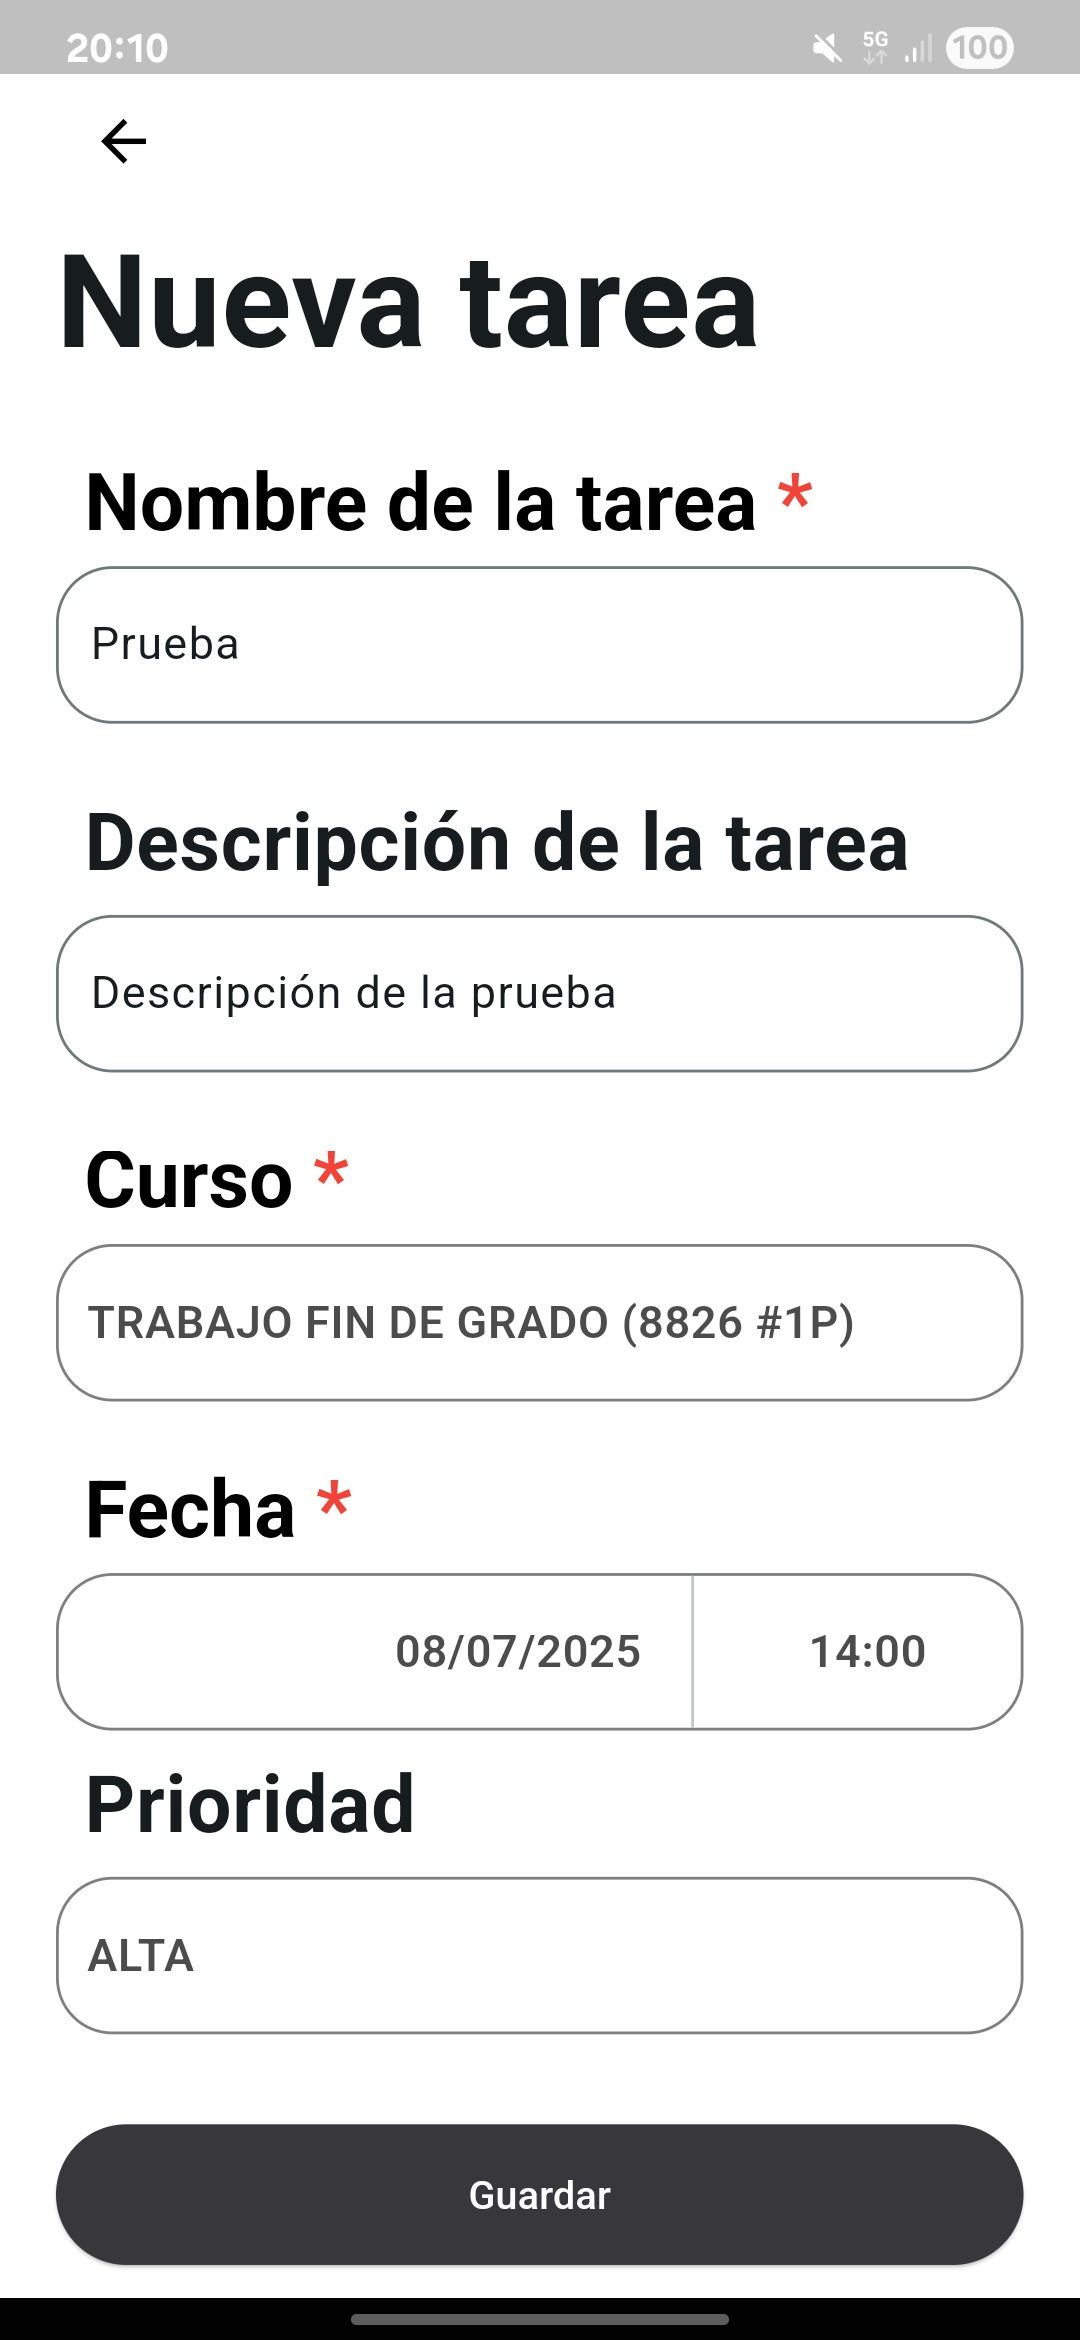
\includegraphics[width=0.5\linewidth]{img/formulario_rellenado.jpg}}
      {\caption{Formulario de creación de tareas personales}
      \label{fig:formulario_rellenado}}
    \hfill
    \ffigbox
     {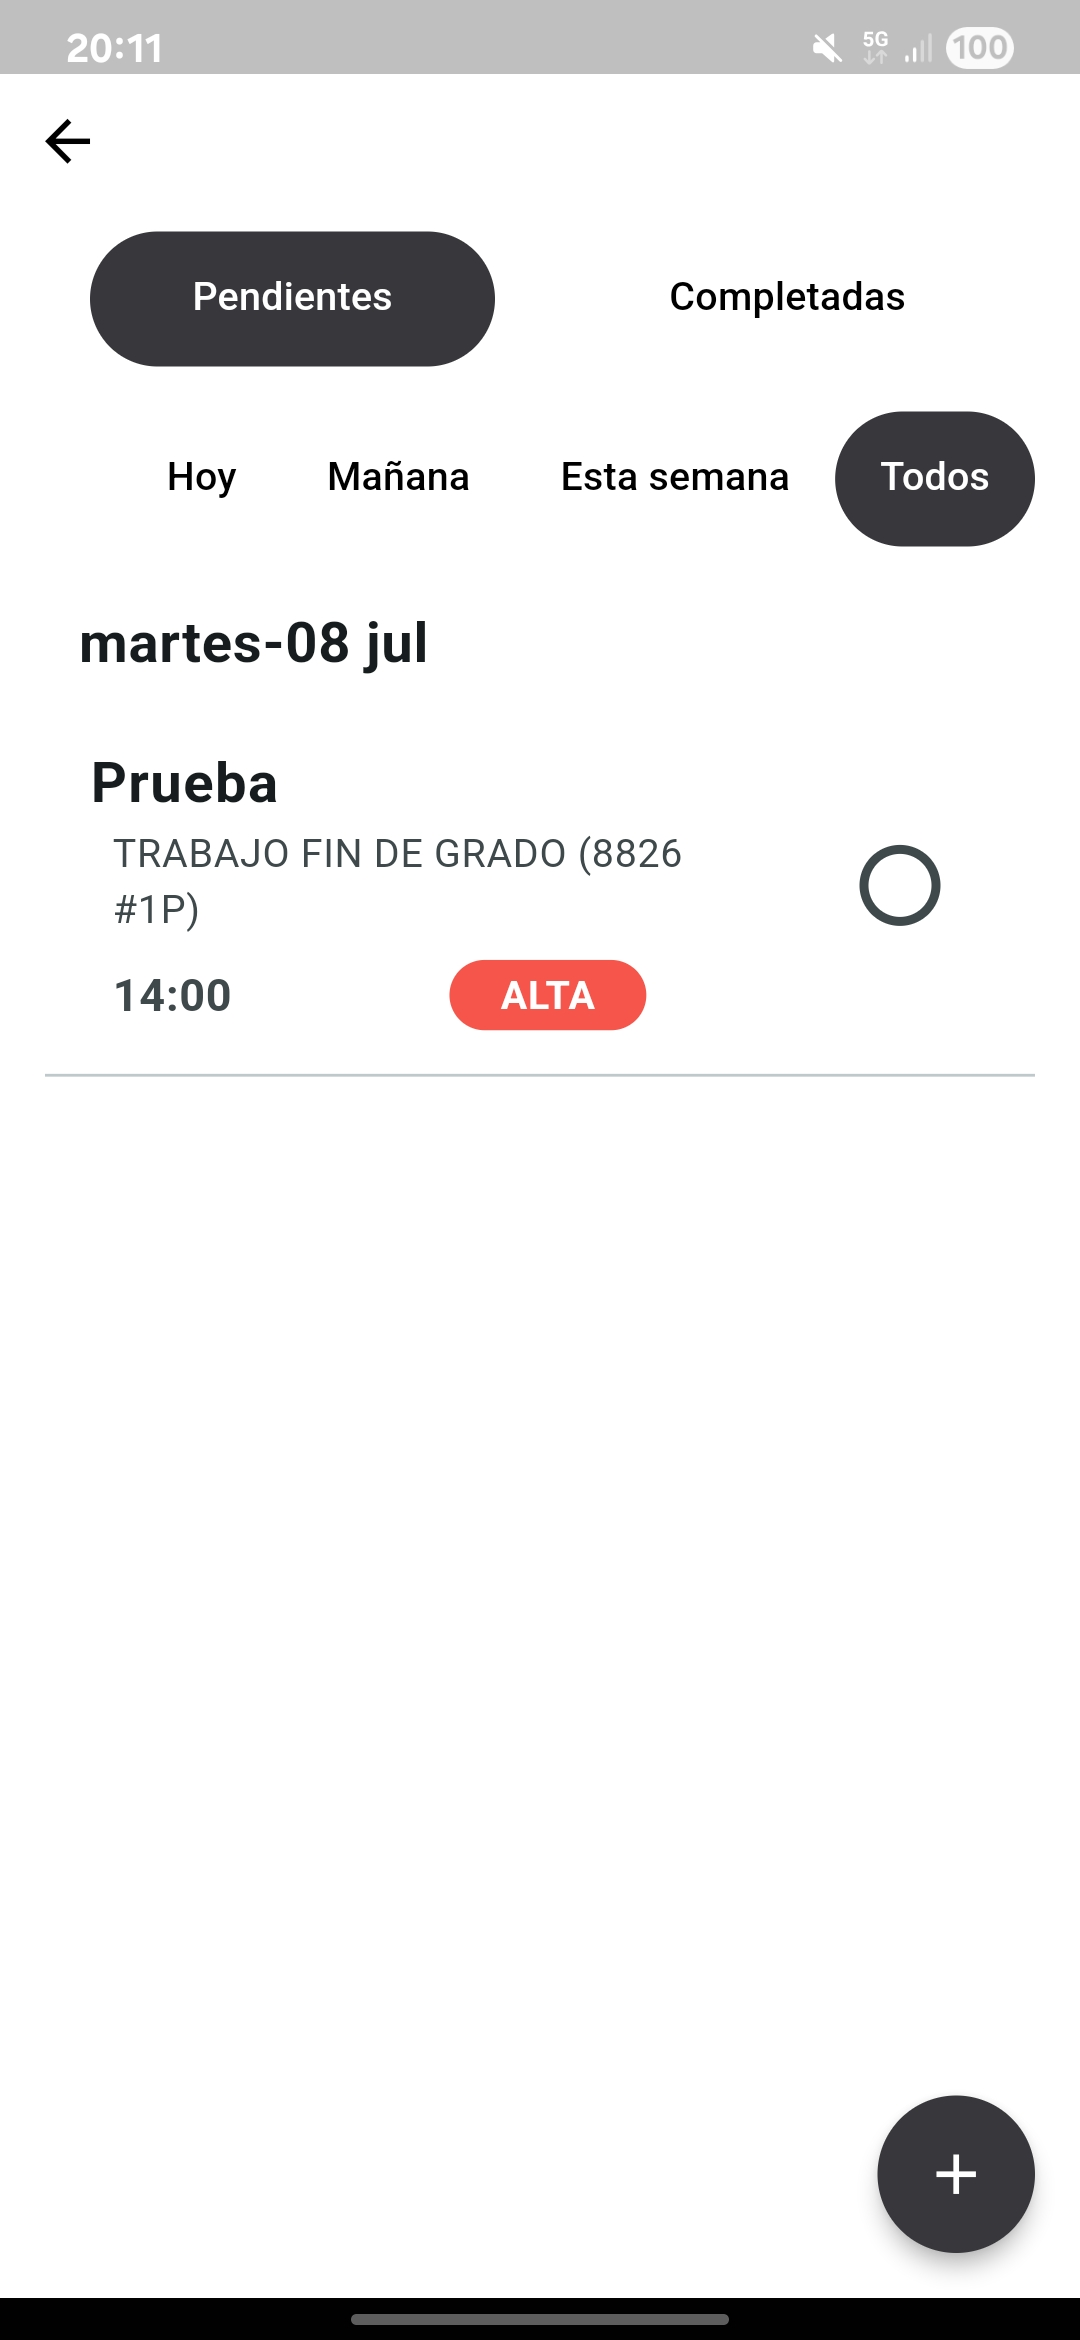
\includegraphics[width=0.5\linewidth]{img/tarea_personal.jpg}}
     {\caption{Tarea personal en sección de \textit{Pendientes}}
     \label{fig:tarea_personal}}
  \end{floatrow}
\end{figure}

Al presionar la tarea personal creada, aparecerá un panel con toda la información de dicha tarea \ref{fig:visualizacion_tarea_personal}.
\begin{figure}[H]
    \centering
    {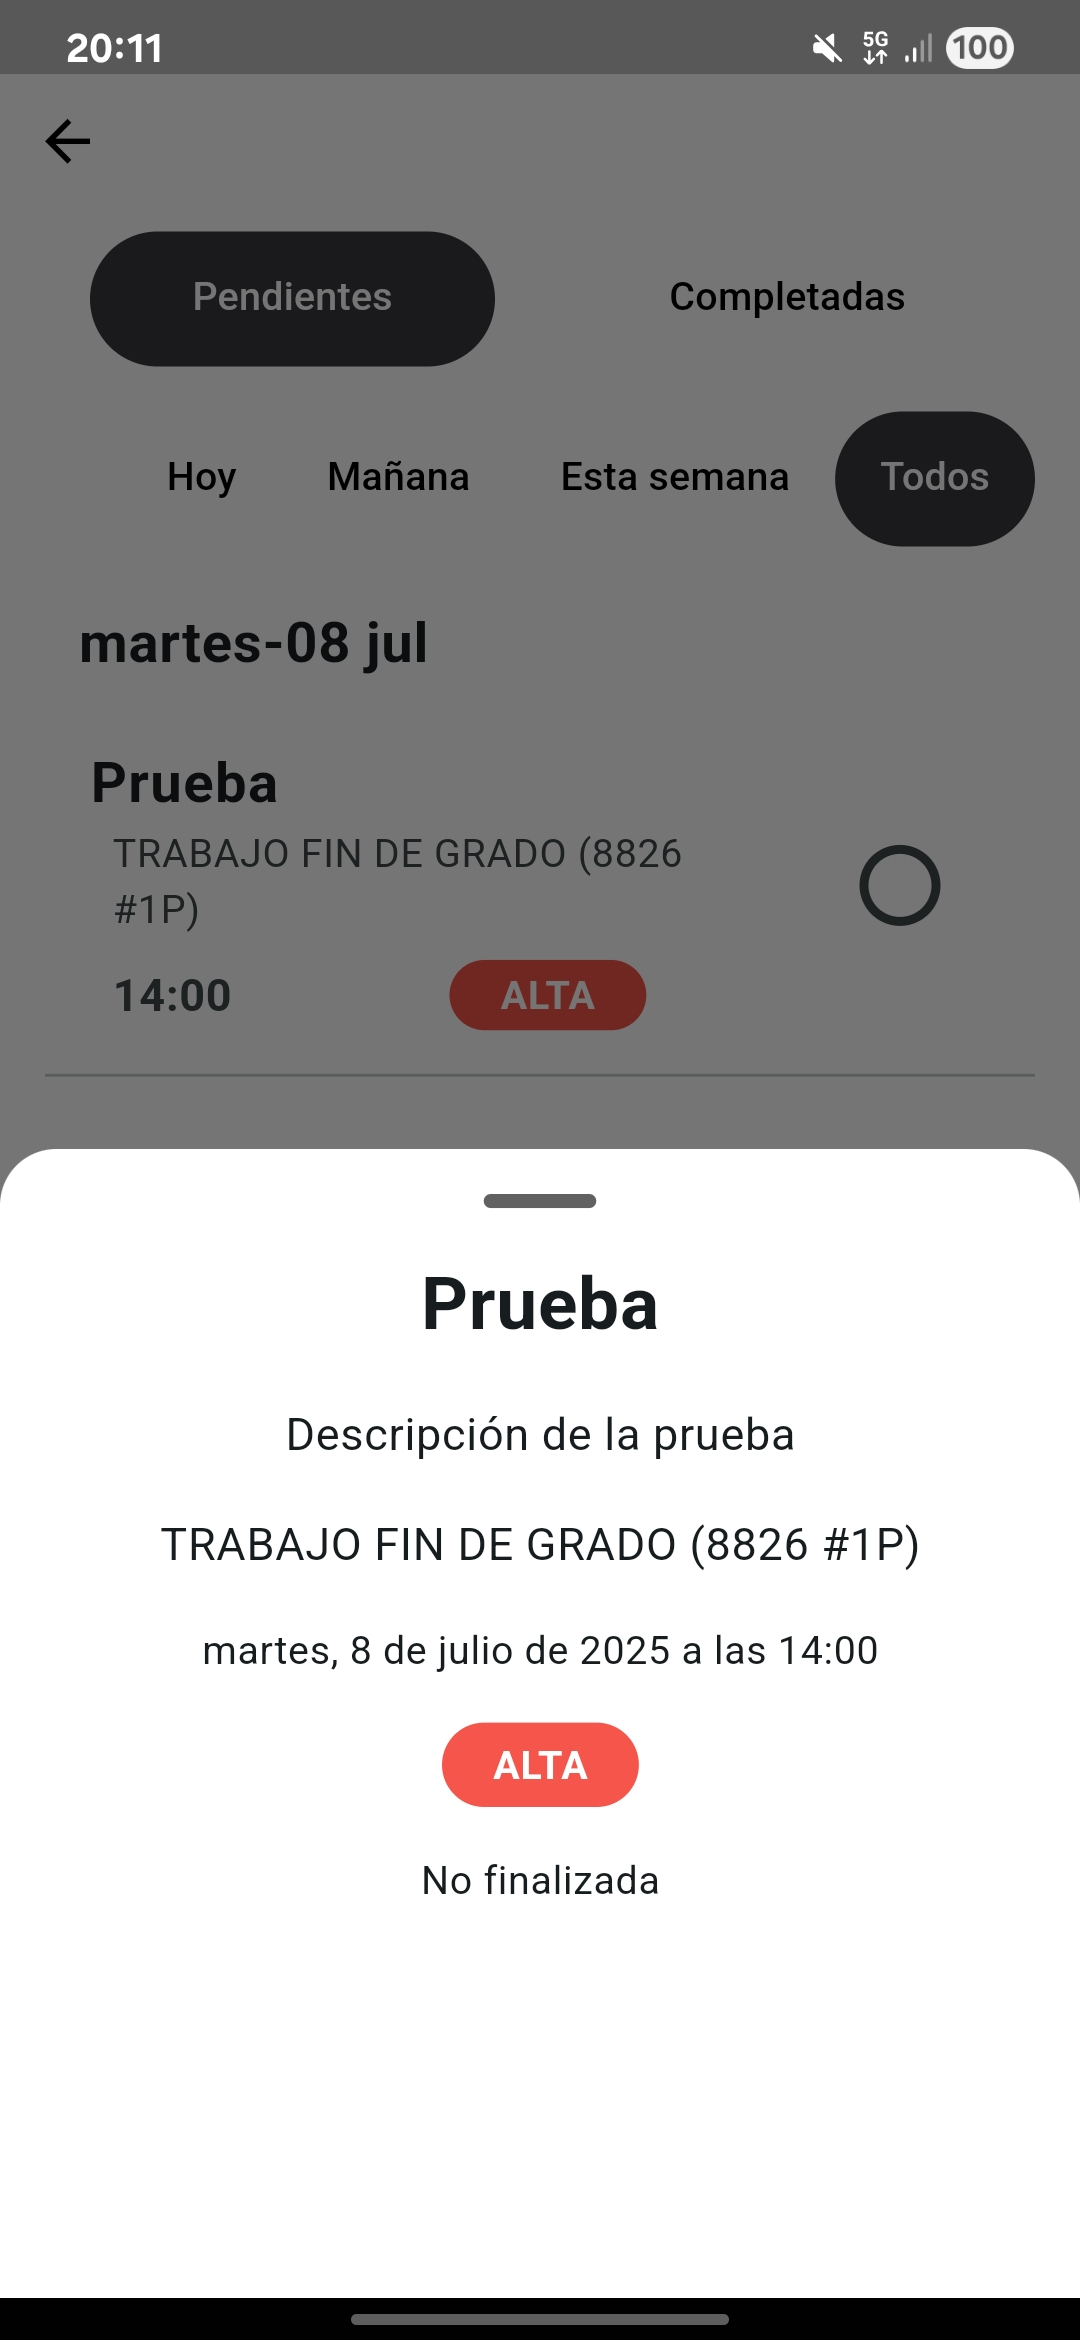
\includegraphics[width=0.25\linewidth]{img/visualizacion_tarea_personal.jpg}}
     {\caption{Panel con información de la tarea personal}
     \label{fig:visualizacion_tarea_personal}}
\end{figure}

El circulo que aparece en la tarea de la pantalla \ref{fig:tarea_personal}, al ser presionado marca la tarea como \textit{Completada} y se moverá directamente a la sección correspondiente.

Por último, si se desliza la tarea de derecha a izquierda, se descubrirá la opción de borrado de la tarea \ref{fig:eliminar_tarea}.
\begin{figure}[H]
    \centering
    {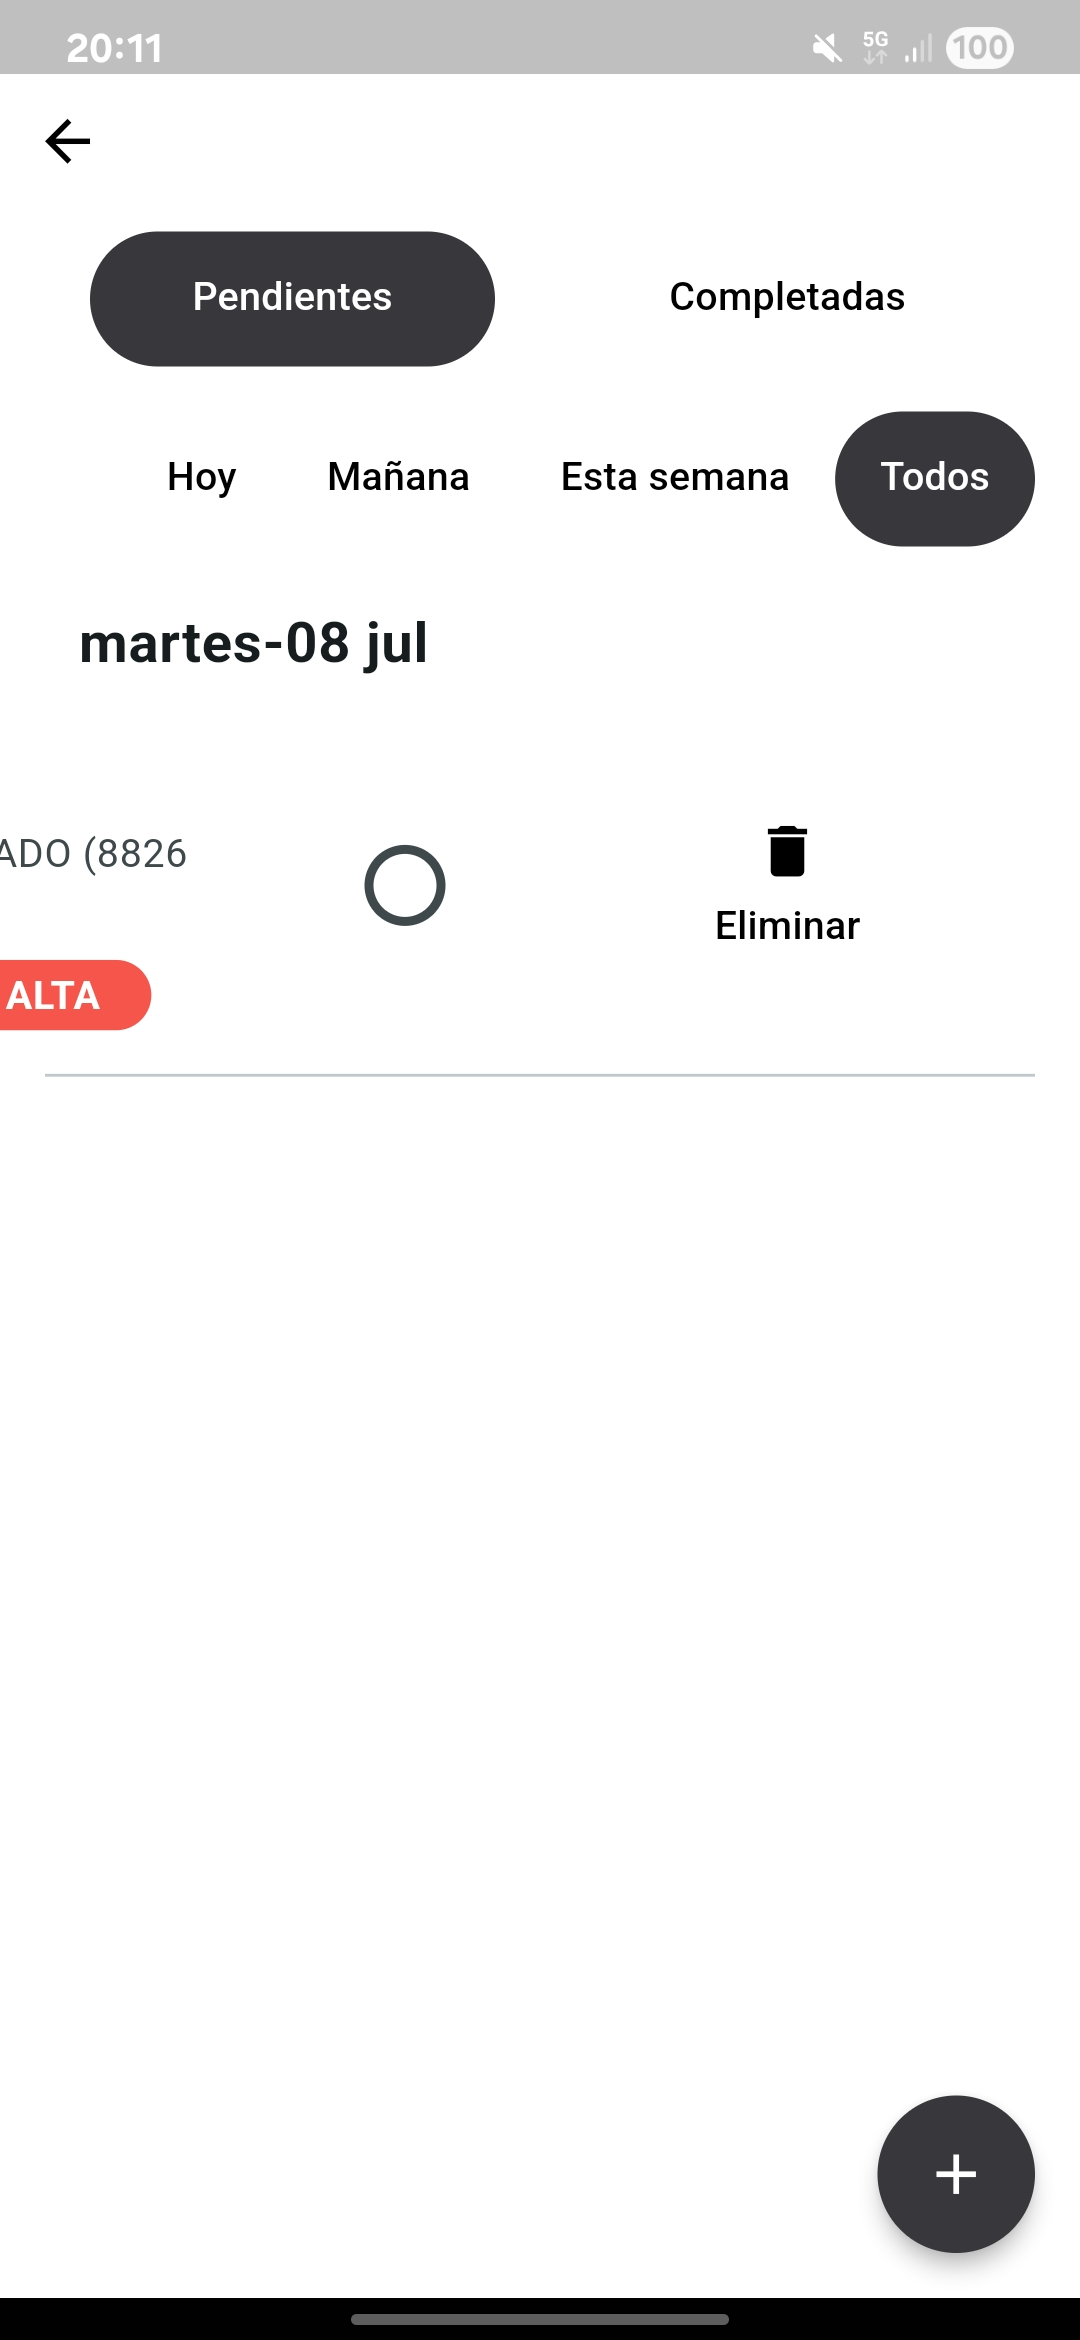
\includegraphics[width=0.25\linewidth]{img/eliminar_tarea.jpg}}
     {\caption{Opción de borrado de la tarea personal}
     \label{fig:eliminar_tarea}}
\end{figure}
\apendice{Anexo de sostenibilización curricular}

\section{Introducción}
Este anexo incluirá una reflexión personal del alumnado sobre los aspectos de la sostenibilidad que se abordan en el trabajo.
Se pueden incluir tantas subsecciones como sean necesarias con la intención de explicar las competencias de sostenibilidad adquiridas durante el alumnado y aplicadas al Trabajo de Fin de Grado.

Más información en el documento de la CRUE \url{https://www.crue.org/wp-content/uploads/2020/02/Directrices_Sosteniblidad_Crue2012.pdf}.

Este anexo tendrá una extensión comprendida entre 600 y 800 palabras.



\bibliographystyle{plain}
\bibliography{bibliografiaAnexos}

\end{document}
